%%%%%%%%%%%%%%%%%%%%%%%%%%%%%%%%%%%%%%%%%%%%%%%%%%%%%%%%%%%%%%%%%%%%%%%%%%%%%
%                                                                           %
%   tuProlog 2.5 Documentation - 2012 edition                               %
%                                                                           %
%   E.Denti, 26/06/12                                                       %
%                                                                           %
%   Strongly based on former contributions by                               %
%   A.Ricci (2000-2002) and G.Piancastelli (2004-2007)                      %                                                %                                                                           %
%%%%%%%%%%%%%%%%%%%%%%%%%%%%%%%%%%%%%%%%%%%%%%%%%%%%%%%%%%%%%%%%%%%%%%%%%%%%%

\documentclass[11pt]{report}
\usepackage[bookmarks=true,bookmarksopen=true,bookmarksnumbered]{hyperref}
\usepackage{graphicx}
\usepackage{fancyvrb}
\usepackage{wrapfig}
%%%%%%%%%%%%%%%%%%%%%%%%%%%%
%\usepackage{float}
%\floatstyle{ruled}
%\newfloat{program}{thp}{lop}
%\floatname{program}{Program}
%%%%%%%%%%%%%%%%%%%%%%%%%%%%

\newcommand\xa[1]{\appendixname~\ref{app:#1}}
\newcommand\labelsec[1]{\label{sec:#1}}
\newcommand\xch[1]{\chaptername~\ref{ch:#1}}
\newcommand\xchp[1]{\chaptername~\ref{ch:#1} \onpagename~\pageref{ch:#1}}
\newcommand\xs[1]{\sectionname~\ref{sec:#1}}
\newcommand\xsp[1]{\sectionname~\ref{sec:#1} \onpagename~\pageref{sec:#1}}
\newcommand\labelssec[1]{\label{ssec:#1}}
\newcommand\xss[1]{\subsectionname~\ref{ssec:#1}}
\newcommand\xssp[1]{\subsectionname~\ref{ssec:#1} \onpagename~\pageref{ssec:#1}}
\newcommand\labelsssec[1]{\label{sssec:#1}}
\newcommand\xsss[1]{\subsectionname~\ref{sssec:#1}}
\newcommand\xsssp[1]{\subsectionname~\ref{sssec:#1} \onpagename~\pageref{sssec:#1}}
\newcommand\labelfig[1]{\label{fig:#1}}
\newcommand\xf[1]{\figurename~\ref{fig:#1}}
\newcommand\xff[2]{\figurenames~\ref{fig:#1}~and~\ref{fig:#2}}
\newcommand\xfp[1]{\figurename~\ref{fig:#1} \onpagename~\pageref{fig:#1}}
\newcommand\labeltab[1]{\label{tb:#1}}
\newcommand\xt[1]{\tablename~\ref{tb:#1}}
\newcommand\xtt[2]{\tablenames~\ref{tb:#1}~and~\ref{ab:#2}}
\newcommand\xtp[1]{\tablename~\ref{tb:#1} \onpagename~\pageref{tb:#1}}
\newcommand\labelenum[1]{\label{enum:#1}}
\newcommand\xen[1]{(\ref{enum:#1})}
\newcommand\xenp[1]{(\ref{enum:#1}) \onpagename~\pageref{enum:#1}}
%******************************************************************************%
\newcommand\bti[1]{\texttt{\textbf{#1}}}
\newcommand\bt[1]{\texttt{#1}}
\newcommand\template[1]{\textit{Template: }\texttt{#1}}
\newcommand\ttit[1]{\texttt{\textit{#1}}}
%******************************************************************************%
\newcommand{\LIA}{\mbox{\textsf{LIA}}}
\newcommand{\aclt}{\mbox{$\mathcal{ACLT}$}}
\newcommand{\respect}{\mbox{\sf{{R}e{S}pec{T}}}}
\newcommand{\luce}{\mbox{\sf{{L}u{C}e}}}
\newcommand{\tucson}{\mbox{\sf{{T}u{CS}o{N}}}}
\newcommand{\alice}{\mbox{\sf{{aliCE}}}}
\newcommand{\apice}{\mbox{\sf{{APICe}}}}
\newcommand{\tuprolog}{\mbox{{\sf{tu}}Prolog}}
%******************************************************************************%
\newcommand\version[1]{\mbox{Document revision: #1}}
\newcommand\creationdate[1]{\mbox{Creation date: #1}}
\newcommand\lastchangesdate[1]{\mbox{Last Changes date: #1}}
\newcommand\noa[2]{\noindent\emph{Note of the author (#1): }#2\\\\}
\newcommand\logo{
    \begin{figure}[tp]
        \begin{center}
            
\includegraphics[width=5cm]{images/logo}
        \end{center}
\end{figure}
}
%******************************************************************************%
\newcommand{\classname}[1]{\texttt{#1}}
\newcommand{\varname}[1]{\texttt{#1}}
\newcommand{\predicate}[1]{\texttt{#1}}
\newcommand{\code}[1]{\texttt{#1}}
\newcommand{\keycap}[1]{\textbf{#1}}
\newcommand{\guibutton}[1]{\textsf{#1}}
\newcommand{\userinput}[1]{\texttt{#1}}
\newcommand{\figref}[1]{\figurename~\ref{#1}}
%******************************************************************************%
\title{{\huge{\bf{\tuprolog{} Manual\\\mbox{ }\\}}}
        \tuprolog{} version: 2.5\\\mbox{ }\\
{\small{\lastchangesdate{2012-06-26}\\}}
}
\author{ \mbox{ }\\ \textsc{Alma Mater Studiorum}---Universit\`{a} di Bologna, Italy
}

\date{}

\begin{document}

\logo

\maketitle

\tableofcontents

%******************************************************************************%
%=======================================================================
\chapter{What is \tuprolog{}}
\label{what-is}
%=======================================================================

\tuprolog{} is an open-source, light-weight Prolog framework for distributed applications and infrastructures, released under the LGPL license, available from \url{http://tuprolog.apice.unibo.it}.

Originally developed in/upon Java, which still remains the main reference platform,
\tuprolog{} is currently available for several platforms/environments:
\begin{itemize}
  \item plain JavaSE;
  \item Eclipse plugin;
  \item Android;
  \item Microsoft .NET.
\end{itemize}
%
While they all share the same core and libraries, the latter features an \emph{ad hoc} library which extends the multi-paradigm approach to virtually any language available on the .NET platform (more on this in Section \xch{dotnet}).

Unlike most Prolog programming environments, aimed at providing a very efficient (yet monolithic) stand-alone Prolog system, \tuprolog{} is explicitly designed to be \emph{minimal}, dynamically \emph{configurable}, straightforwardly \emph{integrated} with Java and .NET so as to naturally support multi-paradigm/multi-language programming (MPP), and \emph{easily deployable}.

\textit{Minimality} means that its core contains only the Prolog engine essentials -- roughly speaking, the resolution engine and some related basic mechanisms -- for as little as 155KB: any other feature is implemented in \textit{libraries}.
%
So, each user can customize his/her prolog system to fit his/her own needs, and no more:
this is what we mean by \tuprolog{} \textit{configurability}---the necessary counterpart of minimality.

Libraries provide packages of predicates, functors and operators, and can be loaded and unloaded in a \tuprolog{} engine both statically and dynamically.
%
Several standard libraries are included in the \tuprolog{} distribution, and are loaded by default in the standard \tuprolog{} configuration; however, users can easily develop their own libraries either in several ways -- just pure Prolog, just pure Java\footnote{The .NET version of \tuprolog{} supports other languages available on the .NET platform: more on this topic in Section \xch{dotnet}}, or a mix of the two --, as we will discuss in \xch{howto-develop-libraries}.

\textit{Multi-paradigm programming} is another key feature of \tuprolog{}.
%
In fact, the \tuprolog{} design was intentionally calibrated from the early stages to support a straightforward, pervasive, multi-language/multi-paradigm integration, so as to enable users to:
\begin{itemize}
  \item using any Java\footnote{For the .NET version: any .NET class, library, object, etc.} class, library, object \emph{directly from the Prolog code}
  (\xch{java-library}) with no need of pre-declarations, awkward syntax, etc., with full support of parameter passing from the two worlds, yet leaving the two languages and computational models totally separate so as to preserve \emph{a priori} their own semantics---thus bringing the power of the object-oriented platform (e.g. Java Swing, JDBC, etc) to the Prolog world for free;

  \item using any Prolog engine \emph{directly from the Java/.NET code} as one would
   do with any other Java libraries/.NET assemblies, again with full support of parameter passing from the two worlds in a non-intrusive, simple way that does not alter any semantics---thus bringing the power of logic programming into virtually \emph{any} Java/.NET application;

  \item augmenting Prolog by defining new libraries \xch{howto-develop-libraries})
  either in Prolog, or in the object-oriented language of the selected platform (again, with a straightforward, easy-to-use approach based on reflection which avoids any pre-declaration, language-to-language mapping, etc), or in a mix of both;

  \item augmenting Java\footnote{This feature is currently available only in the Java version: a suitable extension to the .NET platform is under study.} by defining new Java methods in Prolog (the so-called `P@J' framework---\xch{PJ}), which exploits reflection and type inference to provide the user with an easy-to-use way to implement Java methods declaratively.
\end{itemize}

Last but not least, \textit{easy deployability} means that the installation requirements are minimal, and that the installation procedure is in most cases\footnote{Exceptions are the Eclipse plugin and the Android versions, which need to be installed as required by the hosting platforms.} as simple as copying one archive to the desired folder.
%
Coherently, a Java-based installation requires only a suitable Java Virtual Machine, and `installing' is just copying a single JAR file somewhere---for as much as 474KB of disk usage (yes, minimality is not just a claim here).
%
Of course, other components can be added (documentation, extra libraries, sources..), but are not necessary for a standard everyday use.
%
The file size is quite similar for the Android platform -- the single APK archive is 234KB -- although an Android-compliant install is performed due to Android requirements.
%
The install process is also quite the same on the .NET platform, although the files are slightly larger.
%
The Eclipse platform also requires a different procedure, since plugin installation have to conform to the requirements of the Eclipse plugin manager: consequently, an update site was set up, where the \tuprolog{} plugin is available as an Eclipse feature. Due to these constraints, file size increases to 1.5MB.


In order to manage all these platforms in a uniform way, a suitable \emph{version numbering scheme} was recently introduced:
\begin{itemize}
  \item the fist two digits represent the engine version;
  \item the last (third) digit is platform-specific and accounts for version differences which do not impact on the Prolog engine -- that is, on the
      \tuprolog{} behaviour -- but simply on graphical aspects or platform-specific
      issues or bugs.
\end{itemize}
%
So, as long as the first two digits are the same, a \tuprolog{} application is guaranteed to behave identically on any supported platform.


Finally, \tuprolog{} also supports \textit{interoperability} with both Internet standard patterns (such as TCP/IP, RMI, CORBA) and coordination models and languages.
%
The latter aspect, in particular, is currently developed in the context of the \tucson{} coordination infrastructure \cite{tucson-aamas99,respect-scico2001}, which provides logic-based, programmable tuple spaces (called \emph{tuple centres}) as the coordination media for distributed processes and agents.\footnote{An alternative infrastructure, \luce{} \cite{luce-aamas2001}, developed the same approach in a location-unaware fashion: this infrastructure is currently no longer supported.}



%******************************************************************************%
%=====================================================================
\chapter{Installing \tuprolog{}}
\label{installation}
%=====================================================================

Quite obviously, the installation procedure depends on the platform of choice.
For Java, Microsoft .NET and Android, the first step is to manually download the desired distribution (or even just the single binary file) from the \tuprolog{} web site, \texttt{tuprolog.alice.unibo.it}, or directly from the Google code repository, \texttt{tuprolog.googlecode.com}; for Eclipse the procedure is different, since the plug-in installation has to be performed via the Eclipse Plugin Manager.

As a further alternative, users wishing to have a look at \tuprolog{} and trying it without installing anything on their computer can do so by exploiting the `Run via Java Web Start' option, available on the \tuprolog{} web site.

\section{Installation in Java}

The complete Java distribution has the form of a single \texttt{zip} file which contains everything (binaries, sources, documentation, examples, etc.) and unzips into a multi-level directory tree, similar to the following (only first-level sub-dirs are shown):

\begin{Verbatim}[frame=single, framerule=0.5mm, samepage=true, boxwidth=5cm]
    2p
    |---ant
    |---bin
    |---build
    |   |---archives
    |   |---classes
    |   |---release
    |   |---reports
    |   |---tests
    |---doc
    |   |---javadoc
    |---lib
    |---src
    |---test
    |   |---fit
    |   |---unit
    |---tmp
    |---test
\end{Verbatim}

An alternative distribution, without sources, is also available in the \textit{Download} section of the \tuprolog{} repository: obviously, in this case only a subset of the above folders is present (namely, only \texttt{bin}, \texttt{doc}, \texttt{lib} and \texttt{reports}).

If you are only interested in the Java binaries, just look into the \texttt{build/archives} directory, which contains two JAR files:
%
\begin{itemize}
%
\item \texttt{2p.jar}, which contains everything you need to use \tuprolog{},
  such as the core API, the \texttt{Agent} application, libraries, GUI,
  etc.; this is a runnable JAR, that open the \tuprolog{} IDE when double-clicked.
%
\item \texttt{tuprolog.jar}, which contains only the core part of \tuprolog{},
  namely, what you will need to include in a Java application project to be able to access the \tuprolog{} classes, and write multi-paradigm Java/Prolog applications.
\end{itemize}

The other folders contain project-specific files: \texttt{src} contains all the sources, \texttt{doc} all the documentation, \texttt{lib} the libraries used by the \tuprolog{} project, \texttt{test} the sources for the \tuprolog{} test suite (partly as FIT test, partly as JUnit tests), \texttt{ant} some Ant scripts to automate the build of parts of the \tuprolog{} project, etc.


\section{Installation in .NET}

The complete .NET distribution has also the form of a single \texttt{zip} file containing everything; however, due to the automatic generation of \tuprolog{} .NET binaries via IKVM from Java (more on this in Chapter \ref{ch:mpp-in-dotnet}), the unzipped directory tree is simpler, as there are no sources (and therefore no tests, no ant tasks, etc), except for \texttt{OOLibrary} and Conventions, which are NET-specific and therefore written in C\#.
%
So, the resulting tree is similar to the following:
%
\begin{verbatim}
    2p
    |---build
    |   |---examples
    |   |---lib
    |---OOLibrary
    |   |---Conventions
    |   |---Fixtures
    |   |---OOLibrary
\end{verbatim}
%
Here, too, an alternative distribution, without the OOLibrary and conventions sources, is also available in the \textit{Download} section of the \tuprolog{} repository: again, only a subset of the above folders is present in this case.

The .NET binary, \texttt{2p.exe}, can be found in the \texttt{build} folder.


\section{Installation in Android}

The Android distribution has the form of a single \texttt{apk} file, to be installed via install mechanism provided by the Android OS.
So, unless you are interested in the implementation details, there should be no need to download the whole project distribution.
If, however, you like to do so, you will eventually get to a directory tree similar to the following (only the most relevant first-level sub-folders are shown):
%
\begin{verbatim}
    2p
    |---assets
    |---bin
    |   |---classes
    |   |---res
    |---doc
    |---gen
    |---libs
    |---res
    |---screenshots
    |---src
\end{verbatim}
%
The APK binary can be found into the \texttt{bin} folder.

As for the Java case, the other folders contain project-specific files: in particular, \texttt{src} contains the sources, \texttt{res} the Android resources automatically generated during the project build process, \texttt{libs} the libraries used by this project---mainly, the \texttt{tuprolog.jar} file of the corresponding Java version, imported here as an external dependency.


\section{Installation in Eclipse}

The installation procedure is different for the Eclipse platform due to the need to conform to the Eclipse standard procedure for plug-in installation via Plugin Manager.
Please see the specific section on the \tuprolog{} web site for detailed, screenshot-driven instruction. 
%******************************************************************************%
%=======================================================================
\chapter{Getting Started}
\label{ch:getting-started}
%=======================================================================

\tuprolog{} can be enjoyed from different perspectives:
\begin{enumerate}
  \item as a \textit{Prolog user}, you can exploit its Integrated Development
        Environment (IDE) and Graphical User Interface (GUI) to consult, edit, and run Prolog programs, as you would do with any other Prolog system---and you can do so in any of the supported platforms (Java, .NET, Android, Eclipse).
  \item as a \textit{Java user}, you can include \tuprolog{} in any Java project, in Eclipse or any other IDE of your choice,
        thus bringing the power of Artificial Intelligence to the Java world; the \tuprolog{} API provides many classes and methods for exchanging data between the Java and the Prolog worlds.
        If your goal is to build a hybrid Java+Prolog application to be run from the Prolog side, the \tuprolog{} plugin
        for Eclipse is probably the most practical choice, as the \tuprolog{} perspective provides all the views over the Prolog world in an Eclipse-compliant, effective way.
  \item as a \textit{.NET user}, analogously, you can add \tuprolog{} to any
        Visual Studio project (including the related IKVM libraries, as detailed in Chapter \ref{ch:mpp-in-dotnet}, or just manually compile your .NET application with the necessary DLL files in the build path. The \tuprolog{} API, which is nearly identical to the Java one, provides for proper data exchange
        between the .NET and the Prolog worlds.
  \item finally, as an \textit{Android user}, you can both enjoy the \tuprolog{} app
        to consult, edit, and run Prolog programs, as you would do with any other Prolog system, and --perhaps more interestingly-- exploit the \tuprolog{} Java API for developing Android applications, adding intelligence to your next Android app.
\end{enumerate}

%=======================================================================
\section{\tuprolog{} for the Prolog User}
\label{sec:prolog-user-perspective}
%=======================================================================

As a Prolog user/programmer, you might want to start running your existing programs.
%
There are three ways to do so:
\begin{itemize}
  \item by using the graphical \tuprolog{} GUI (both in Java and .NET)
  \item by using the console-based \tuprolog{} CUI  (Java only)
  \item by using the \texttt{Agent} class to execute a Prolog program in a `batch' form---that is, running the program provided as a text file (Java only).
\end{itemize}

The first two forms are rather obvious: after starting the GUI/CUI, you will get a rather standard graphical/character-based Prolog user interface (Figure \ref{fig:tuprologGUICUI}).

The GUI includes an editing pane with syntax highlighting, a toolbar providing facilities to load/save/create theories, load/unload libraries, and show/hide the the debug information window; at the bottom, the status bar provides information, as detailed below.

The GUI can be launched either by double-clicking the \tuprolog{} executable (\texttt{2p.jar} in Java, \texttt{2p.exe} in .NET), or by manually issuing the commands

\texttt{java -cp \emph{dir}/2p.jar alice.tuprologx.ide.GUILauncher}

\noindent or

\texttt{2p.exe}

\noindent in .NET, respectively.

Analogously, the command-line CUIconsole (available in Java only) can be launched by issuing the command:

\texttt{java -cp \emph{dir}/2p.jar alice.tuprologx.ide.CUIConsole}

\noindent The CUIconsole can be quitted issuing the standard \texttt{halt.} command.

% ED 2.7.3
\begin{figure}
\centering
  \includegraphics[width=300px]{images/tuprologIDE.png}\\
  \includegraphics[width=300px]{images/tuprologCUI.png}\\
  \caption{The standard \tuprolog{} GUI and CUI. (The upper right button, opening SpyFrame window, is present only from version 2.7.2 onwards; the \textit{call tree} tab view in the bottom dialog is to be included in version 2.7.3).}\label{fig:tuprologGUICUI}
\end{figure}

The third form, available in Java only, is basically an auxiliary tool to batch-execute a Prolog program: it takes the name of a text file containing a Prolog theory as its first (mandatory) argument and optionally the goal to be solved as its second argument, then starts a new Prolog virtual machine, performs the demonstration, and ends.
%
The \texttt{Agent} tool is invoked from the command line as follows:

\texttt{java -cp \textit{dir}/2p.jar alice.tuprolog.Agent \textit{theoryfile}
\{\textit{goal}\}}

\noindent For instance, if the file \verb|hello.pl| contains the mini-theory:

\texttt{go :- write('hello, world!'), nl.}

\noindent the following command causes its execution:

\texttt{java -cp \textit{dir}/2p.jar alice.tuprolog.Agent hello.pl go.}

\noindent resulting in the string \texttt{hello, world!} being printed on the standard output.

\noindent Alternatively, the goal to be proven can be embedded in the Prolog source by means of the \texttt{solve} directive, as follows (Figure \ref{fig:tuprologAgent}):

\texttt{:- solve(go).}\\
\indent\texttt{go :- write('hello, world!'), nl.}

\noindent Quite obviously, in this case no second argument is required.

\begin{figure}
\centering
  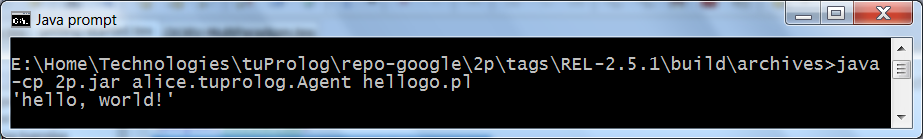
\includegraphics[width=300px]{images/tuprologAgent.png}
  \caption{The \tuprolog{} Agent tool.}\label{fig:tuprologAgent}
\end{figure}

%------------------------------------------------------
\subsection{Editing theories}
\label{sec:editing-theories}
%------------------------------------------------------

The editing area allows multiple theories to be created and modified at the same time, by allocating a tab with a new text area for each theory.
%
The text area provides syntax highlighting for comments, string and list literals, and predefined predicates.
%
Undo and Redo actions are supported through the usual \keycap{Ctrl}+\keycap{Z} and \keycap{Ctrl}+\keycap{Shift}+\keycap{Z} key bindings.

\begin{figure}
\centering
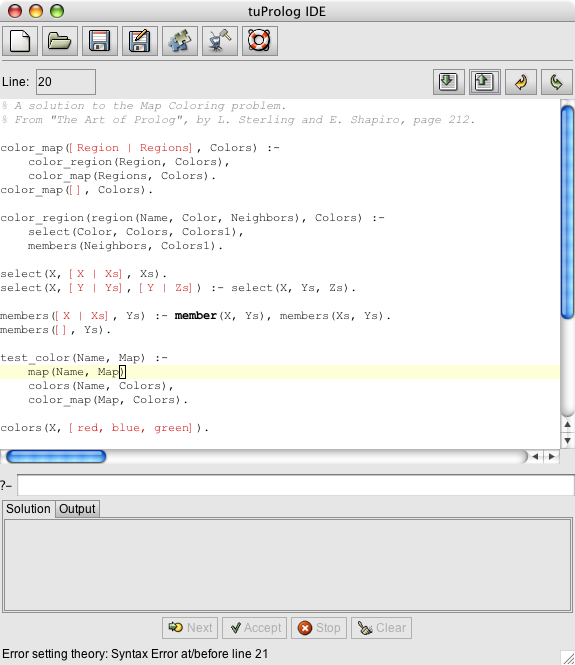
\includegraphics[width=7cm]{images/syntaxErrorFound}
\caption{Syntax error found when setting a theory.}
\label{fig:syntax-error-found}
\end{figure}

\begin{figure}
\centering
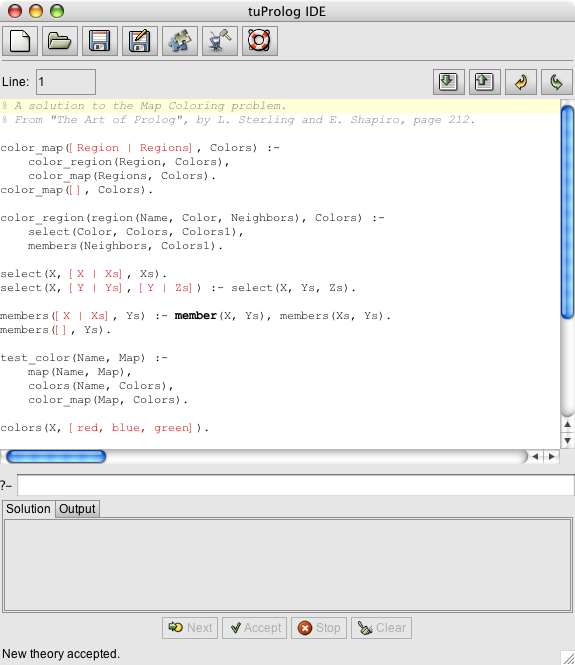
\includegraphics[width=7cm]{images/setTheorySucceeded}
\caption{Set theory operation succeeded.}
\label{fig:set-theory-succeeded}
\end{figure}

The toolbar contains four buttons: two are used to upload/download a theory to/from the Prolog engine, two support the classical Undo/Redo actions.
%
Explicit uploading/downloading of theories to/from the Prolog engine is a consequence of \tuprolog{}'s choice to maintain a clear separation between the engine and the currently-viewed theories: in this way,
\begin{itemize}
  \item theories can be edited without affecting the engine content: they can also be in an inconsistent state, since syntax checking is performed only upon loading;
  \item changes in the current database performed by the Prolog program via the \texttt{assert}/\texttt{retract} do not affect the theory shown in the editor, which maintains the original user theory.
\end{itemize}
%
Accordingly, the \textit{set theory} button uploads the text in the editor window to the engine, while the \textit{get theory} button downloads the current engine theory (possibly changed by the program) from the engine to a new editor tab.

However, for the user convenience, a logical shortcut is provided that automatically uploads the current theory to the engine whenever a new query is issued: obviously, if the theory is invalid, the query will not be executed.
%
Manual uploading is still needed whenever the theory in the editor window is modified via other other means than the built-in editor---for instance, after a \predicate{consult/1} goal\footnote{%
  If a Prolog theory contains an \texttt{include} directive or a \texttt{consult} command to load other sub-files,
  \tuprolog{} versions up to 2.6 require either the absolute sub-file name, or a relative path referred to the engine's
  base folder. From version 2.7 on, an enhanced mechanism enables a Prolog file located in \texttt{someOtherFolder} (that is, a folder other than the current one) to consult/include another file from the current
  folder by simply issuing a \texttt{consult(someOtherFile)} command, delegating the \tuprolog{} engine for searching the file in all the subfolders of the current working folder. See also Section \ref{ssec:relative-paths-consulting-subfiles-in-java-project}.
}, or via other editors.

The status bar at the bottom of the window reports information such as the cursor line number or syntax errors when setting an invalid theory.
%
For instance, Figure \ref{fig:syntax-error-found} shows the error message due to a missing dot at line 8, while Figure \ref{fig:set-theory-succeeded} shows the status message after the error has been corrected, and the theory successfully uploaded.

%------------------------------------------------------
\subsection{Solving goals}
\label{sec:solving-goals}
%------------------------------------------------------

The console at the bottom of the window contains the \textit{query textfield} and a multi-purpose, tabbed information panel.

The \textit{query textfield} is where to write and execute queries: the leftmost (\guibutton{Solve}) button triggers the engine to find the first (and then the subsequent) solution(s) interactively, while the rightmost (\guibutton{Solve All}) button forces the engine to find all the solutions at once.
%
Pressing the \keycap{Enter} key in the textfield has the same effect as pressing the \guibutton{Solve} button.

\begin{figure}
\centering
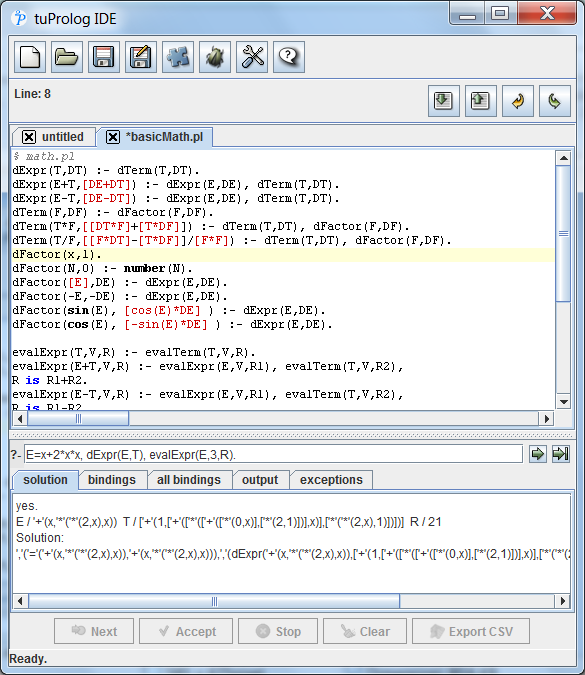
\includegraphics[width=7cm]{images/gui-solutions}
\caption{The solutions tab showing the query solution.
(The \textit{call tree} tab view is to be included in version 2.7.3).}
% 2.7.3
\label{fig:gui-solutions}
\end{figure}

\begin{figure}
\centering
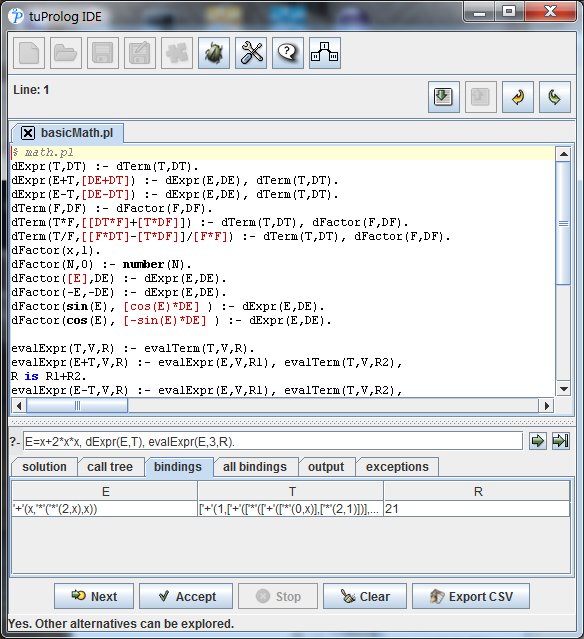
\includegraphics[width=7cm]{images/gui-bindings}
\caption{The bindings tab showing the bindings of query solution.
(The \textit{call tree} tab view is to be included in version 2.7.3).}
% 2.7.3
\label{fig:gui-bindings}
\end{figure}

The subsequent area below contains six panes:
%
\begin{itemize}
\item the \textit{solution} pane shows the query solutions (see Figure \ref{fig:gui-solutions}): proper control buttons are provided to iterate through multiple solutions;

% 2.7.3
% \item the \textit{call tree} pane shows a graphical view of the last-solved query (see Figure \ref{fig:gui-calltree});

\item the \textit{binding} and the \textit{all bindings} panes show the variable bindings in tabular form, for a single solution or for all solutions, respectively (see Figure \ref{fig:gui-bindings}); here, too, proper control buttons are provided to clear the bindings pane and export the tabular data in a convenient CSV format;

\item the \textit{output} pane shows the output performed by the program via \texttt{write} and other console I/O predicates (Figure \ref{fig:gui-output}).
    Please note that output performed by Java methods -- that is, methods invoked on Java objects via \classname{JavaLibrary} -- are \textit{not} captured and displayed in this view: for further information on this topic, refer to Section \ref{sec:java-library}.
    %
    Again, control buttons are provided to clear the output pane.

\item the \textit{exceptions} pane shows the exceptions raised during the query demonstration: if exceptions are triggered, it gains focus automatically and is color-highlighted for the user convenience (Figure \ref{fig:gui-exceptions}).
\end{itemize}

% 2.7.3
%\begin{figure}
%\centering
%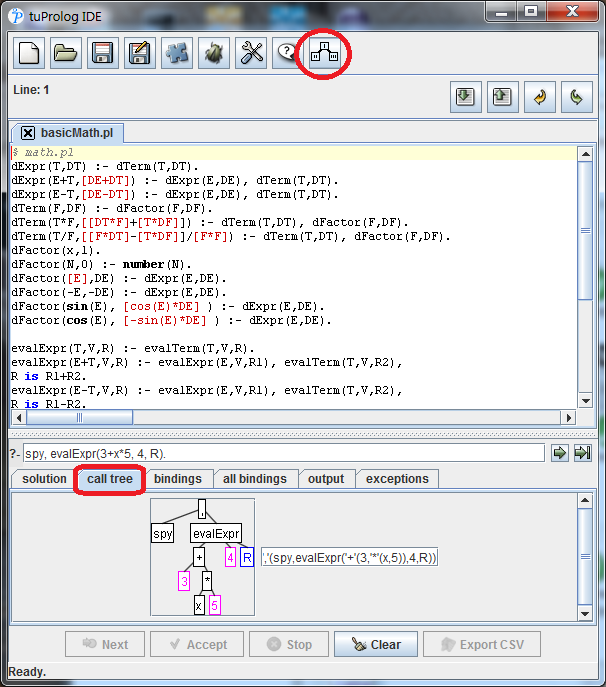
\includegraphics[width=7cm]{images/gui-calltree1}
%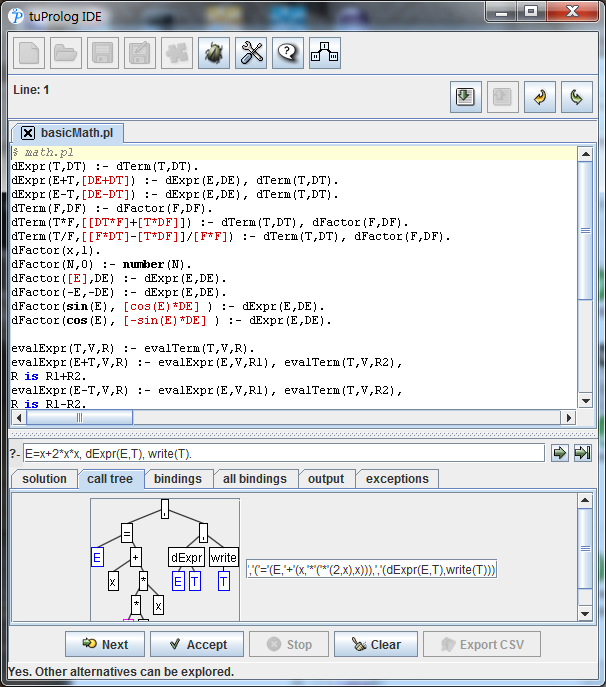
\includegraphics[width=7cm]{images/gui-calltree2}
%\caption{The call tree tab showing a graphical view of the last-solved query.}
%\label{fig:gui-calltree}
%\end{figure}

\begin{figure}
\centering
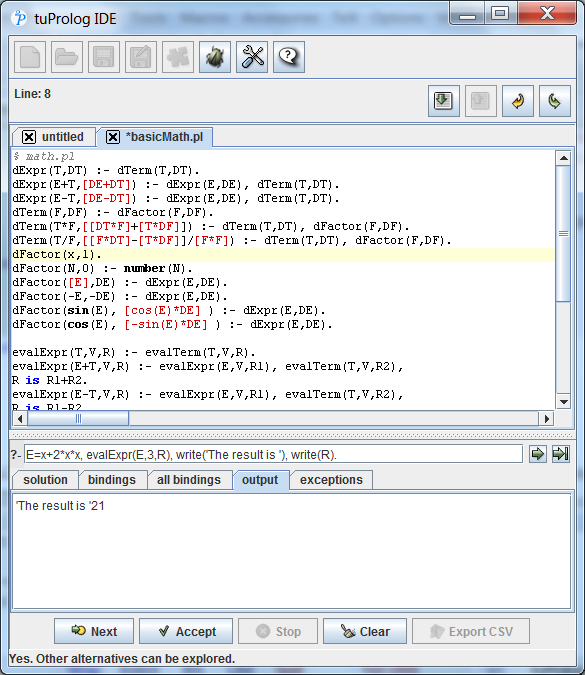
\includegraphics[width=7cm]{images/gui-output}
\caption{The output tab showing the query printing.
(The \textit{call tree} tab view is to be included in version 2.7.3).}
% 2.7.3
\label{fig:gui-output}
\end{figure}

\begin{figure}
\centering
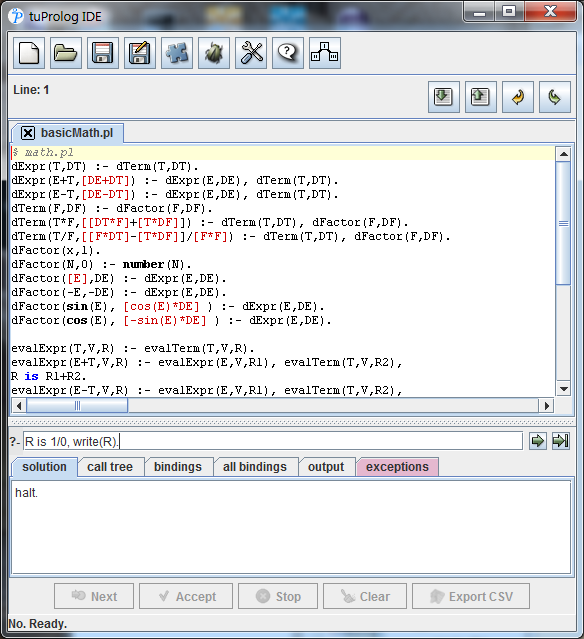
\includegraphics[width=7cm]{images/gui-exceptions}
\caption{The exceptions tab gaining focus and showing raised exceptions.
(The \textit{call tree} tab view is to be included in version 2.7.3).}
% 2.7.3
\label{fig:gui-exceptions}
\end{figure}
Query and answers are stored in chronological order, and can be explored by means of \keycap{Up} and \keycap{Down} arrow keys from the query input textfield.

The \guibutton{Stop} button makes it possible to stop the engine if a computation takes too long or a bug in the theory is causing an infinite loop.
%(Note: like most Prolog systems, \tuprolog{} does not normally perform \textit{occur check}, for performance reasons; this check can be enabled via the proper built-in predicate---see Section \ref{sec:basic-library} for details.)

With respect to this issue, it is worth noting that, unlike most Prolog systems, \tuprolog{} performs the so-called \textit{occur check} systematically: so, \texttt{unify\_with\_occurs\_check/2} and \texttt{=/2} behave identically (see Section \ref{sec:basic-library}).

%------------------------------------------------------
\subsection{Debugging support}
\label{ssec:debugging-support}
%------------------------------------------------------

Debug support in \tuprolog{} is actually limited compared to other professional Prolog systems: however, \textit{warnings} and \textit{spy information} are available.

To this end, the \guibutton{View Debug Information} button opens the Debug window which lists \textit{i)} all the warnings, produced by events such as the attempt of redefining a library predicate, and \textit{ii)} the step-by-step spy information of the engine computation during a goal demonstration.

Warnings are always active, while spy notification has to be explicitly enabled (and disabled) via the built-in \predicate{spy/0} (\predicate{nospy/0}) predicate.
%
Figure \ref{fig:gui-debug} shows an example of spy information for a goal: by default, information is presented in a collapsed form, but single nodes (or all the nodes) can be expanded using the toolbar buttons, to access more detailed information.

\begin{figure}
\centering
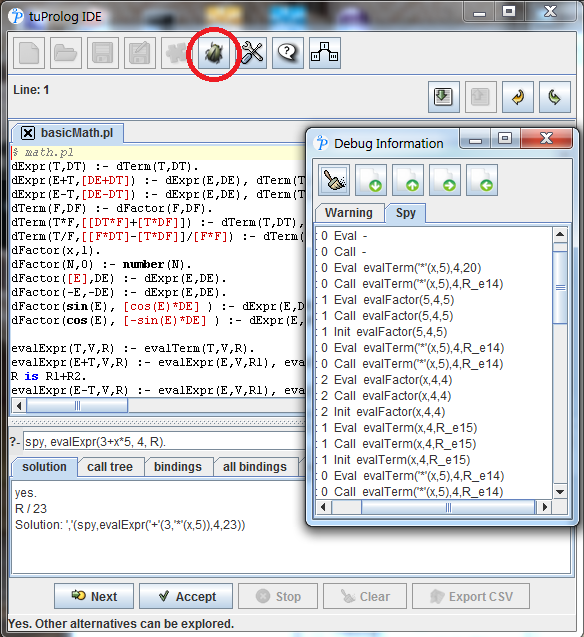
\includegraphics[width=7cm]{images/gui-debug}
\caption{Debug Information View after the execution of a goal.}
\label{fig:gui-debug}
\end{figure}

As of \tuprolog{} 2.7.2, an alternative approach is available via the \textit{Spy Frame} window, which can be opened clicking on the top-right, tree-like button (Figure \ref{fig:gui-spyframe}).
This window makes it possible to \textit{graphically reproduce} the solving process of the query, step-by-step: so, while the above debug view operates in real time during the resolution, the SpyFrame operates \textit{after} the query has been solved, basically re-solving the same query one step at a time\footnote{%
    SpyFrame exploits its own Prolog engine and execution thread for this purpose, so no side effects are caused in the main window even if the SpyFrame is closed unexpectedly.}
%
Each time the Next button is pressed, the simulation advances of \textit{N} steps, where \textit{N} is the number shown in the adjacent textfield (default 1).
Figure \ref{fig:gui-spyframe} shows some screenshots captured in different phases of a rather complex demonstration.

\begin{figure}
\centering
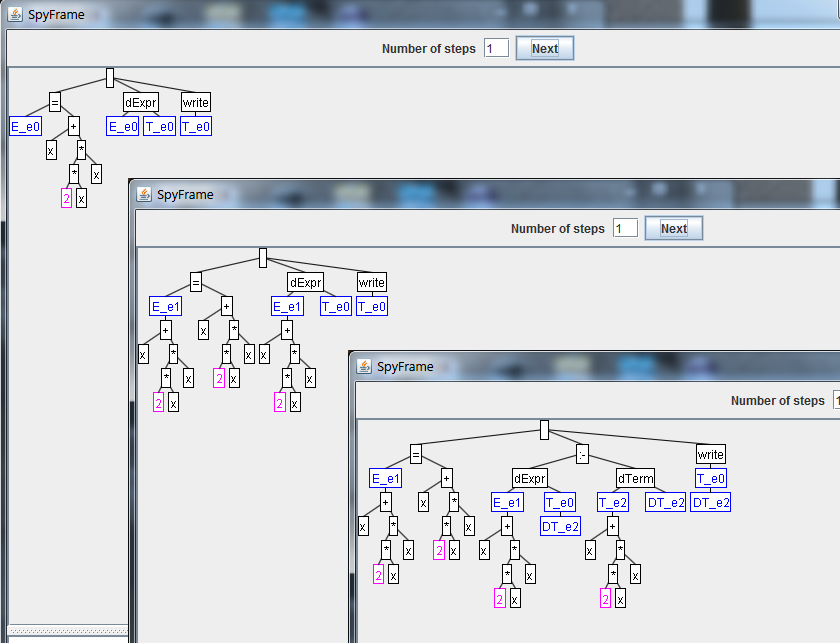
\includegraphics[width=7cm]{images/gui-spyframe1}
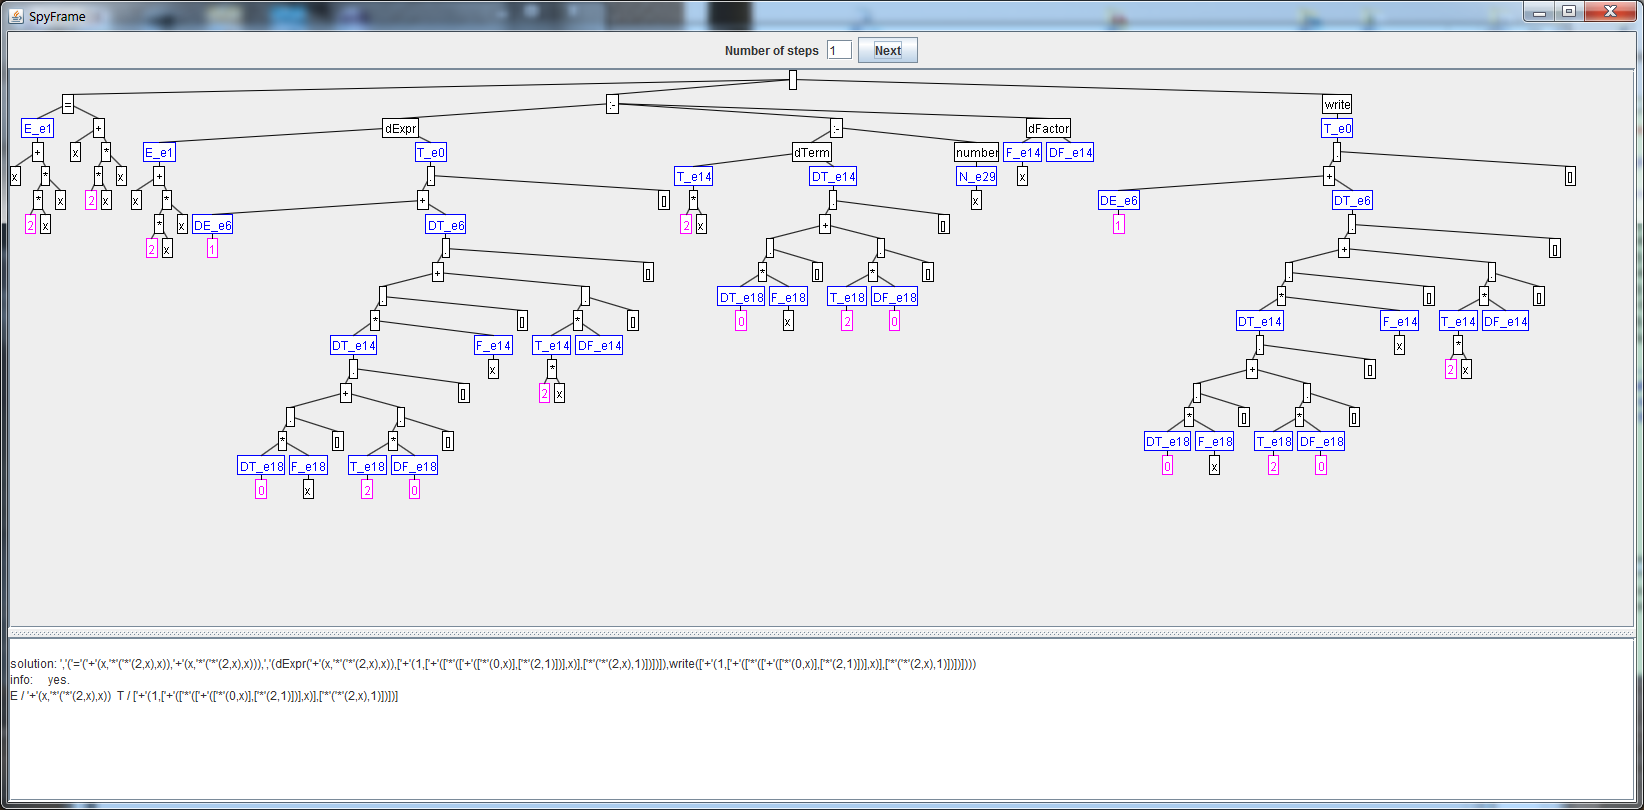
\includegraphics[width=7cm]{images/gui-spyframe2}
\caption{The Spy Frame (new in \tuprolog{} 2.7.2) showing a step-by-step graphical view of the last-solved query.}
\label{fig:gui-spyframe}
\end{figure}


%------------------------------------------------------
\subsection{Dynamic library management}
\label{ssec:dynamic-library-management}
%------------------------------------------------------

As anticipated above, \tuprolog{} engines are dynamically extensible via \textit{libraries}: each library can provide its own set of new built-in
predicates and functors, as well as a related theory.
%
By default, the standard set of libraries is loaded into any newly-created engine, but the library set of each engine can be easily modified via the \textit{Library Manager}, which is displayed by pressing the \guibutton{Open Library Manager} button in the toolbar (Figure \ref{fig:gui-library-manager}).

\begin{figure}
\centering
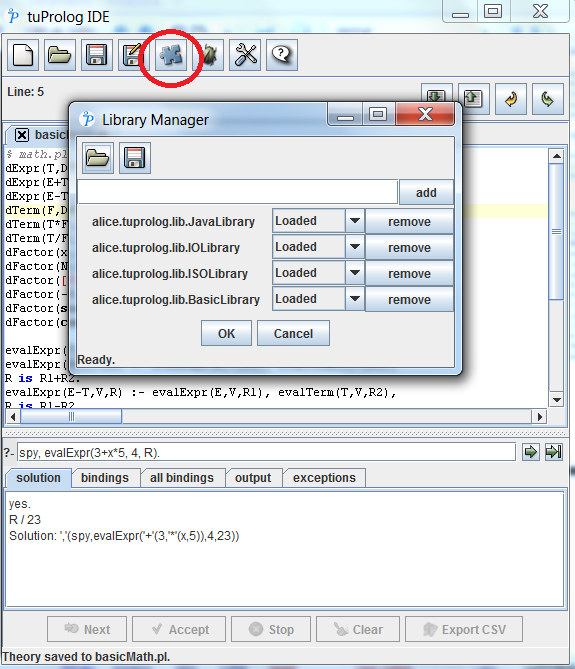
\includegraphics[width=7cm]{images/gui-library-manager}
\caption{The Library Manager window.}
\label{fig:gui-library-manager}
\end{figure}

This dialog displays the list of the currently loaded libraries---by default,
\classname{BasicLibrary}, \classname{IOLibrary}, \classname{ISOLibrary}, \classname{JavaLibrary}.
%
Other libraries can be added by providing the fully qualified name of the library class in the textfield, and pressing the \guibutton{Add} button: the added library will be displayed with an initial \textit{Unloaded} status.
The new library must be in the current class path for \tuprolog{} to find it; alternatively, the \textit{Browse..} button can be used to locate a library class anywhere in the file system (furhter information on class loading issues can be found in Section \ref{ssec:library-loading-issues}).
%
Quite clearly, class loading constraints also apply to any further class possibly needed by the library, too: a library will not be added to the manager/loaded into the engine if any of its required classes cannot be found.

The library manager takes into account the effects of \verb|load_library/1|-\verb|/2| and \verb|unload_library/1|-\verb|/2| predicates/directives, too: so, for instance, after a goal such as \verb|load_library('TestLibrary'), test(X).|, a new entry for \verb|TestLibrary| would be displayed.

If a library cannot be added, or its loading into the engine fails (for instance, due to an invalid class name, or the class not being in the current class paths, or a class not extending the \classname{alice.tuprolog.Library} class, etc.), an error message will be displayed in the status bar.

The bottom icons in Figure \ref{fig:gui-library-manager} are used to load and store preferences.

\noindent Finally, the \guibutton{config} button in the \tuprolog{} GUI opens the configuration dialog (Figure \ref{fig:gui-configuration}), which provides access to a set of options and tunings.

\begin{figure}
\centering
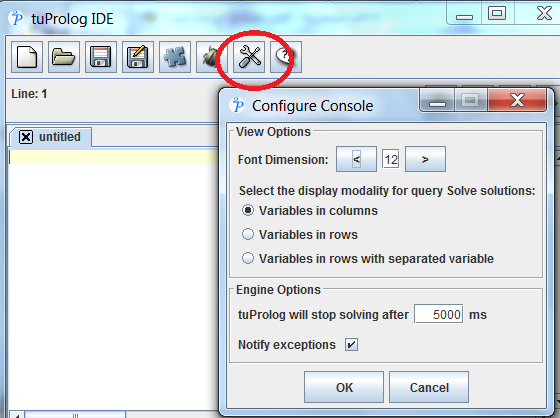
\includegraphics[width=7cm]{images/gui-config}
\caption{The configuration window.}
\label{fig:gui-configuration}
\end{figure}

%------------------------------------------------------
\subsection{Input from console}
\label{ssec:input-from-console}
%------------------------------------------------------

Until \tuprolog{} 2.7.x, an input from the standard input stream (e.g. via some of the IOLibrary/ISOIOLibrary input predicates, like \texttt{read}), could only be performed in the CUIConsole: any attempt to perform keyboard reading on the GUIConsole led to exception, because the underlying \emph{stdin} was uncaptured by the Prolog GUI.
This behaviour has been fixed in \tuprolog{} 2.8: henceforth, if a query performs a read operation from the standard input stream, the GUIConsole intercepts the request and shows the corresponding dialog (Figure \ref{fig:gui-InputFromConsole}). More on this in Section \ref{sec:io-library}.

\begin{figure}
\centering
  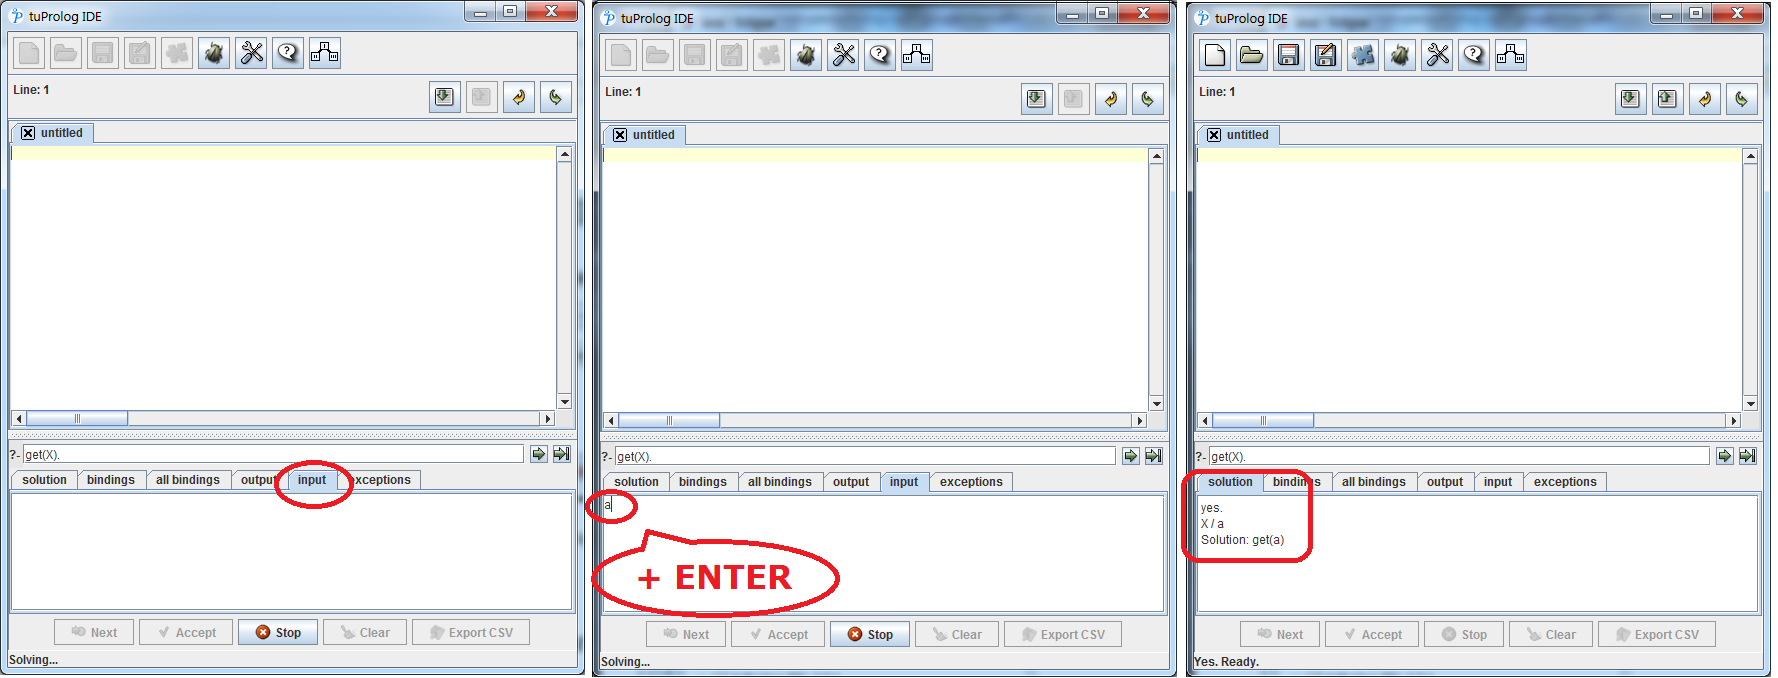
\includegraphics[width=7cm]{images/gui-InputFromConsole.png}
  \caption{Keyboard input management in the case of a read operation from the standard input.}\label{fig:gui-InputFromConsole}
\end{figure}

%=======================================================================
\section{\tuprolog{} for the Java Developer}
\label{sec:java-user-perspective}
%=======================================================================

As anticipated above, the Java developer can include \tuprolog{} in any of his projects, exploiting the \tuprolog{} API to access the Prolog engine(s) from his/her Java program: in fact, if your goal is just to embed intelligence in your Java application, all you need is adding the \texttt{tuprolog.jar} library (or the \texttt{2p.jar} library in the case you need also the extra classes) to your Java project, and develop normally---\tuprolog{} will be seen as any other referenced JAR archive.

However, if your goal is to develop a hybrid Java+Prolog application to be run from the Prolog side -- that is, where Java objects and methods are called from a Prolog program -- the \tuprolog{} plugin for Eclipse is probably the best choice, since it adds a specific \textit{tuprolog perspective} specifically suited for the needs of the Java/Prolog user (Figure \ref{fig:tuprologPluginGUI}).

\begin{figure}
\centering
  \includegraphics[width=300px]{images/tuprologPluginGUI.png}
  \caption{The \tuprolog{} plugin GUI for Eclipse.}\label{fig:tuprologPluginGUI}
\end{figure}

This perspective is mainly designed to support the development of multi-language, multi-paradigm applications (see Chapters \ref{ch:mpp-in-java}, \ref{ch:mpp-in-dotnet}), but can also be used as a standard Prolog console, writing (or loading) the Prolog theory in the editor and writing the query in the proper textfield---although the direct use of the \tuprolog{} GUI is probably faster for this purpose.

To use \tuprolog{} in Eclipse, one first needs to create a new \tuprolog{} project, and add a new theory file (\texttt{*.pl}) to the project.
%
To this end:%, three procedures are possible:
\begin{itemize}
  \item either select \texttt{New $>$ Project} from the Package Explorer's context menu, then select the \texttt{tuProlog} item;
  \item or, select \texttt{File $>$ New $>$ Other $>$ tuProlog $>$ tuProlog Project} from the main menu;
  \item or, press the \textit{New tuProlog Project} buttons in the \tuprolog{} toolbar (Figure \ref{fig:plugin1}.
\end{itemize}

In any case, a dialog appears (Figure \ref{fig:plugin2}) which prompts for the project name (default: \texttt{My\_Prolog\_Project}) and the desired Prolog libraries (the default set is proposed).

\begin{figure}
\centering
  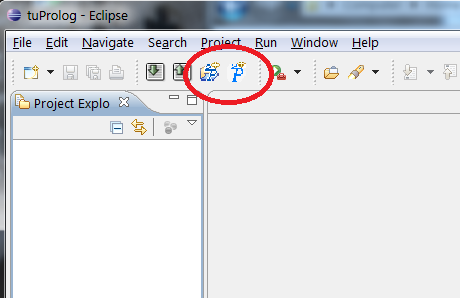
\includegraphics[width=200px]{images/plugin1.png}
  \caption{The \tuprolog{} toolbar}\label{fig:plugin1}
\end{figure}

\begin{figure}
\centering
  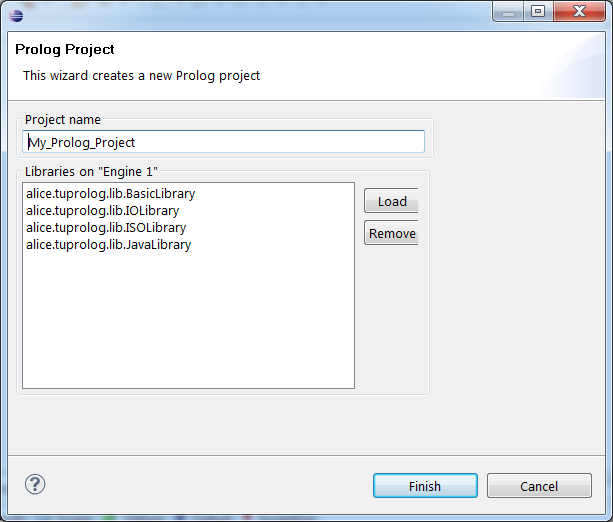
\includegraphics[width=200px]{images/plugin2.png}
  \caption{new \tuprolog{} project}\label{fig:plugin2}
\end{figure}

\begin{figure}
\centering
  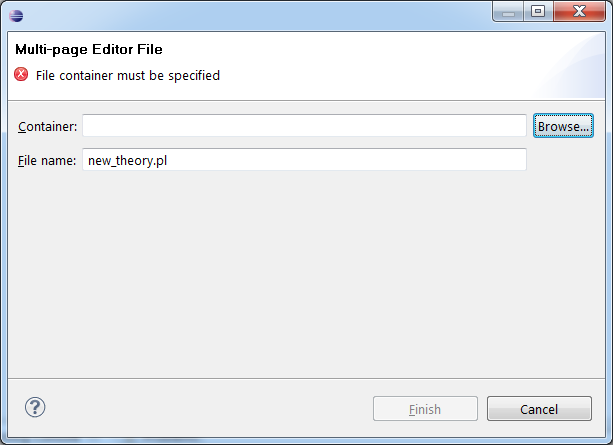
\includegraphics[width=200px]{images/plugin3.png}
  \caption{new \tuprolog{} file}\label{fig:plugin3}
\end{figure}

\begin{figure}
\centering
  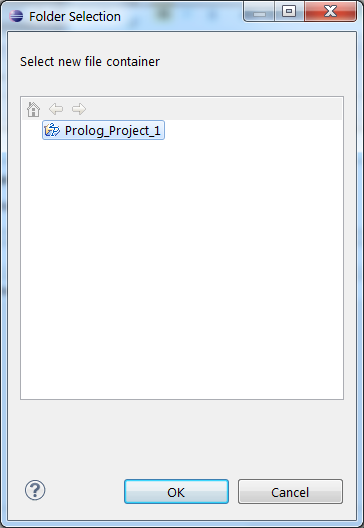
\includegraphics[width=200px]{images/plugin4.png}
  \caption{new \tuprolog{} file $>$ Browse...}\label{fig:plugin4}
\end{figure}

\begin{figure}
\centering
  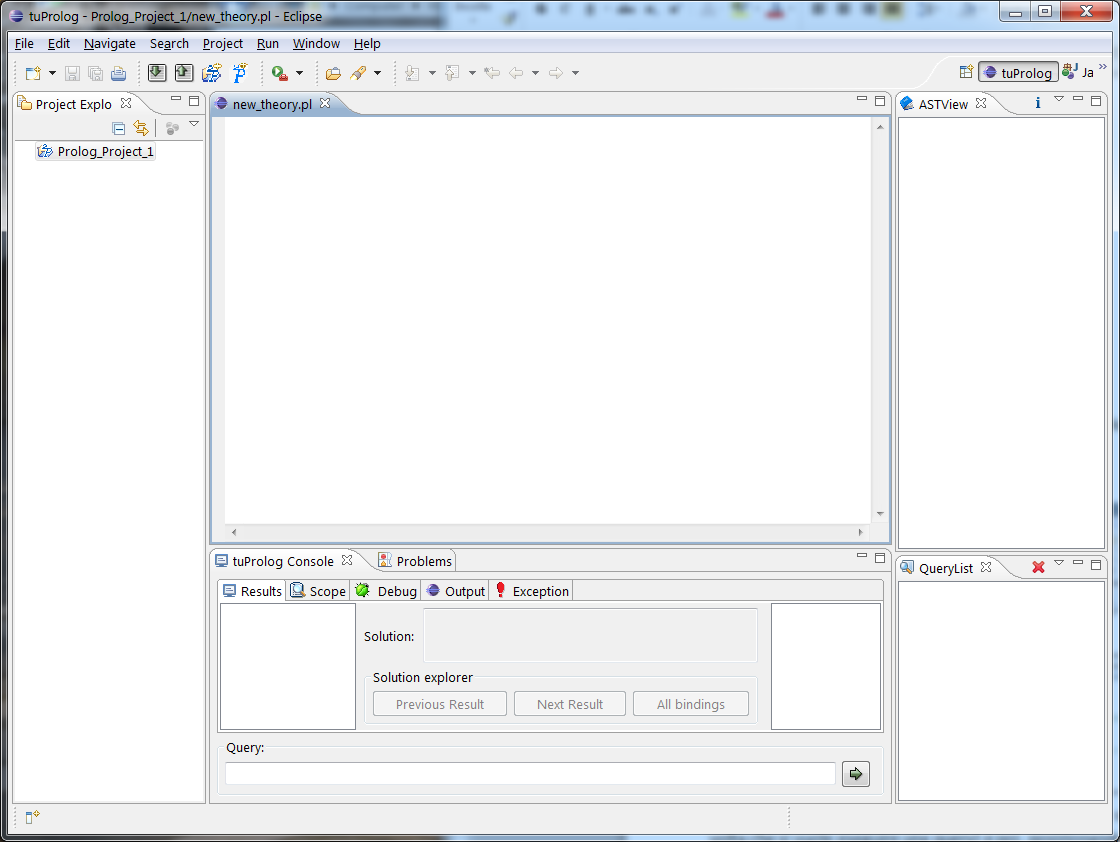
\includegraphics[width=200px]{images/plugin5.png}
  \caption{the \tuprolog{} perspective}\label{fig:plugin5}
\end{figure}

\begin{figure}
\centering
  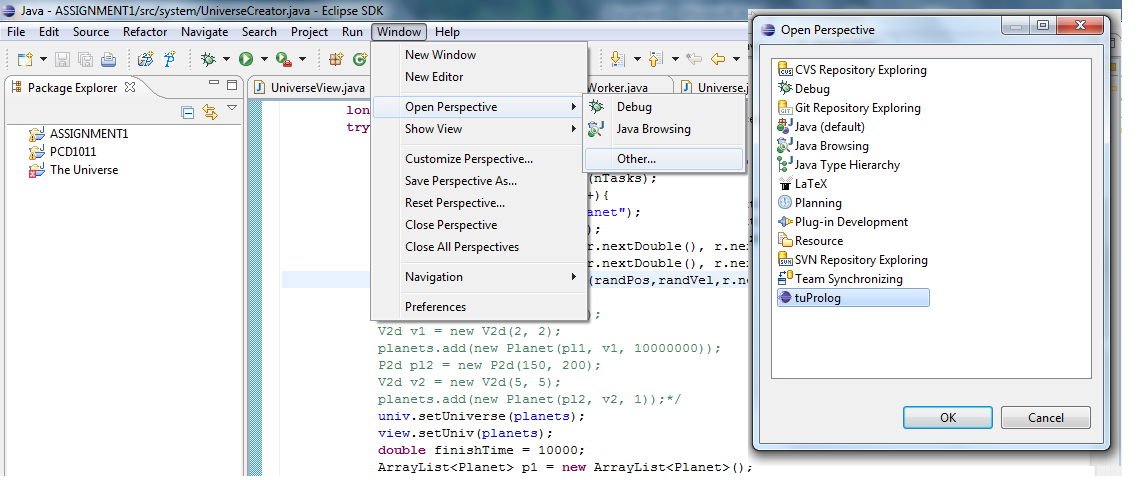
\includegraphics[width=200px]{images/plugin6.png}
  \caption{opening the \tuprolog{} perspective}\label{fig:plugin6}
\end{figure}

Pressing the \textit{New tuProlog File} button, a dialog appears which asks for the theory name (default: \texttt{new\_theory.pl}) and the file container, i.e. the tuProlog project where the new file has to be added (Figure \ref{fig:plugin3}); this is a mandatory argument. Pressing the \textit{Browse..} button, a new dialog proposes the current \tuprolog{} projects (Figure \ref{fig:plugin4}); again, the same result can be achieved via menu selection  (\texttt{File $>$ New $>$ Other $>$ tuProlog $>$ tuProlog Theory}). After confirming, the \tuprolog{} perspective automatically opens (Figure \ref{fig:plugin5}). Again, the same result can be achieved via the \texttt{Window $>$ Open Perspective} menu (Figure \ref{fig:plugin6}).

Once the theory has been written (or loaded), the theory file must be saved, either clicking the save icon in the toolbar, or choosing the \texttt{File $>$ Save} option, or hitting CTRL+S on the keyboard; this is mandatory before issuing any query.
The query can be written in the bottom console, and is executed either by pressing the Enter key, or by clicking the \textit{Solve} button.


\begin{figure}
\centering
  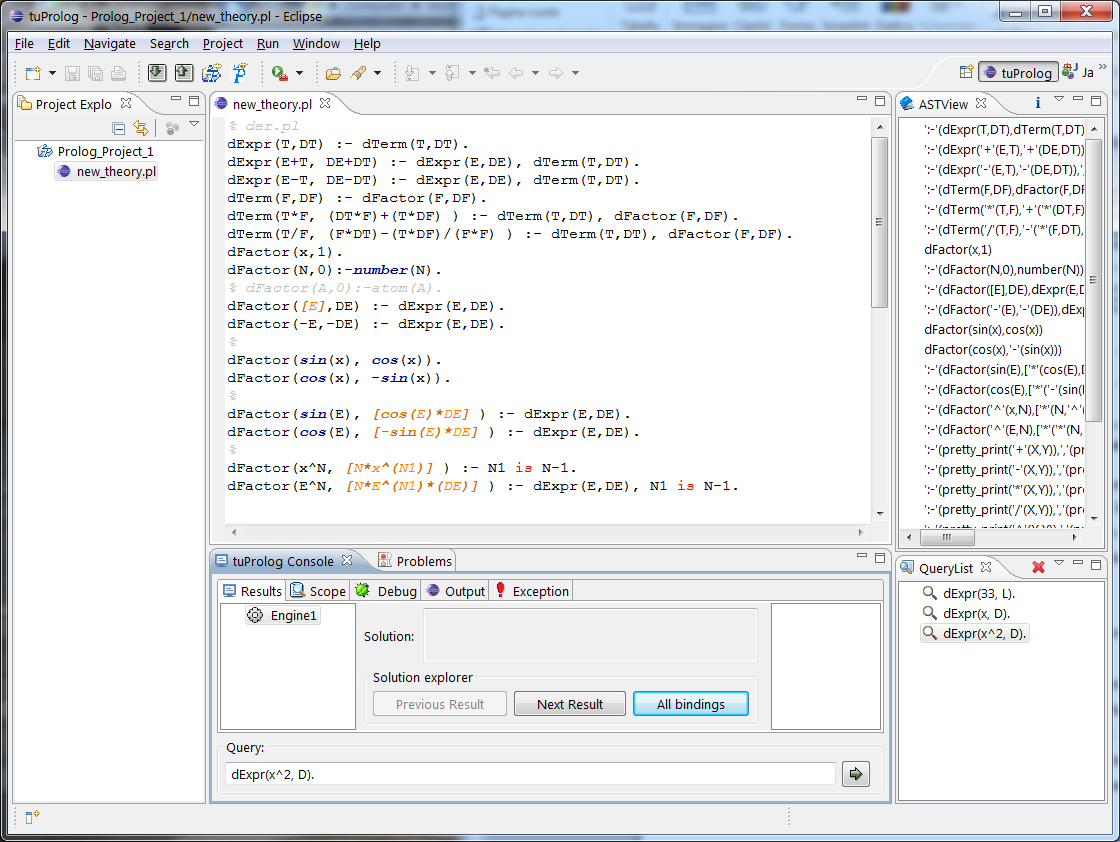
\includegraphics[width=4cm]{images/plugin7.png}
  \caption{executing queries, available views}\label{fig:plugin7}
\end{figure}

\begin{figure}
\centering
  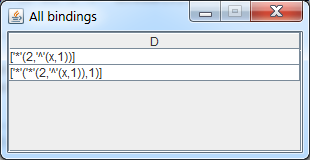
\includegraphics[width=200px]{images/plugin8.png}
  \caption{all variable bindings}\label{fig:plugin8}
\end{figure}

\begin{figure}
\centering
  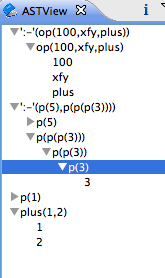
\includegraphics[width=200px]{images/plugin9.png}
  \caption{AST view (expanded)}\label{fig:plugin9}
\end{figure}

\begin{figure}
\centering
  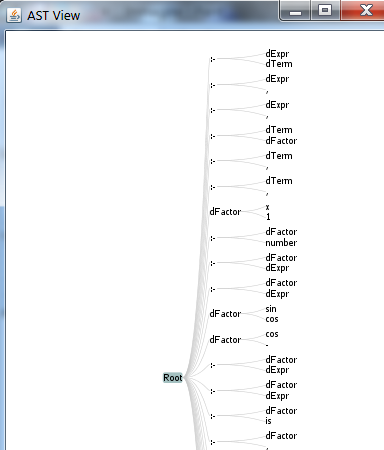
\includegraphics[width=200px]{images/plugin10.png}
  \caption{AST view (big term, expanded)}\label{fig:plugin10}
\end{figure}

The query results are shown in different views (Figure \ref{fig:plugin7}):
\begin{itemize}
  \item the \tuprolog{} Console view reports the query results: the variable bindings are also available pressing the \textit{All bindings} button (Figure \ref{fig:plugin8}).
  \item the Output view shows the program output messages;
  \item the QueryList view on the left side reports the list of all he executed queries, which can then be re-selected and re-executed in a click;
  \item the AST view shows the (dynamic) set of current clauses: pressing the \texttt{i} icon, a graphical view of the Abstract Syntax Tree produced by the Prolog parser is shown (Figures \ref{fig:plugin9} and \ref{fig:plugin10}).
\end{itemize}

It is worth highlighting that multiple \tuprolog{}  engines can be handled simultaneously: each engine can be selectively loaded with each own set of libraries and theories, and can be separately queried.
%
Moreover, in case of undeclared terms, a direct warning is issued in the plugin editor  (Figure \ref{fig:plugin11}).

\begin{figure}
\centering
  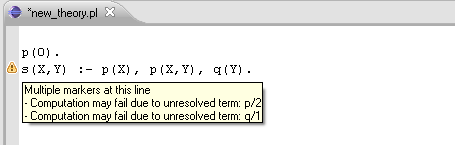
\includegraphics[width=200px]{images/plugin11.png}
  \caption{warning for undeclared terms}\label{fig:plugin11}
\end{figure}

%=======================================================================
\section{\tuprolog{} for the .NET Developer}
\label{sec:dotnet-user-perspective}
%=======================================================================

Since \tuprolog{}.NET is the result of an automatic conversion of the Java bytecode via IKVM \cite{ikvm}, everything in the Prolog user experience is identical whether the .NET or the Java GUI is used (see Section \ref{sec:prolog-user-perspective} above).

The .NET developer, however, can exploit \tuprolog{} in a .NET project, accessing its API from a program written in potentially any language available in the .NET platform.
%
Since no plugin is available for the de-facto standard tool used by most .NET programmers (i.e., Microsoft Visual Studio), there is no immediate way to see \tuprolog{} at work from within Visual Studio; however, the \tuprolog{} libraries can be easily added as external references for exploiting the available APIs, as one would do with any other library or third-party software.

For specific information about multi-paradigm programming in the context of the .NET platform, please refer to Chapter \ref{ch:mpp-in-dotnet}.


%=======================================================================
\section{\tuprolog{} for the Android User}
\label{sec:android-user-perspective}
%=======================================================================

Since \tuprolog{} is written in Java, the Java-Android developer wishing to include \tuprolog{} in an Android project can proceed very similarly to the Java developer, adding \texttt{tuprolog.jar} to the project libraries---though no plugin is available for this platform.

The Prolog-Android user, instead, can take advantage of the \tuprolog{} app, which shares the same core and libraries as the standard Java version, the only difference being the redesigned GUI--with special regard to the interaction with the file system.

Upon the application loading, the splash screen appears, immediately followed in a few seconds by the \textit{Home Activity} (Figure \ref{fig:android12}, left).
%
At the top, the name of the selected theory is reported (none at the beginning); below is the query textfield.
%
Four buttons enable the user to execute a query, ask for the next solution (when applicable), show the current solution and view the output console.
%
The menu button triggers the pop-up shown in Figure \ref{fig:android12} (right), whose main feature is \textit{List Theories}.

\begin{figure}
\centering
  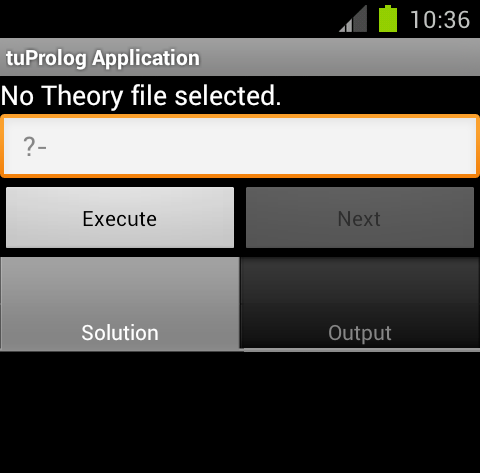
\includegraphics[width=200px]{images/android1.png}
  
\includegraphics[width=200px]{images/android2.png}
  \caption{Home Activity (left) and its pop-up menu (right).}\label{fig:android12}
\end{figure}

Indeed, in \tuprolog{} for Android theories are not loaded directly in the Prolog engine from the file system, as in the standard Java version: rather, following Android recommendations, a \textit{theory database} mediator is provided, so as to separate the loading of a theory from its validity check---the latter being performed only when the theory is actually selected for being loaded into the engine. In this way, invalid theories (possibly incomplete, work-in-progress theories) can seamlessly be stored in the theory database, independently of their invalid nature.

So, theories of interest must be first loaded into the theory database (Figure \ref{fig:android34}, left): then, the theory to be actually loaded will be selected from such theories.
%
More precisely, to add a theory to the database, the menu option \textit{Import Theory to Database} is provided (Figure \ref{fig:android34}, right): a new activity opens that lets you browser the device's file system (Figure \ref{fig:android56}, left). Only the files that can be actually selected for addition to the theory database are shown: after a theory is successfully imported, the activity remembers the path for the next time, so as to make it faster to import multiple files.

\begin{figure}
\centering
  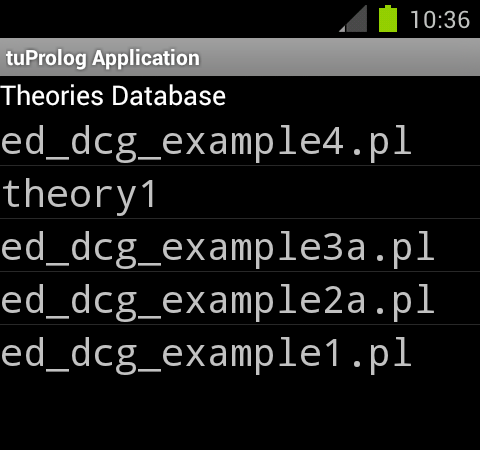
\includegraphics[width=150px]{images/android3.png}
  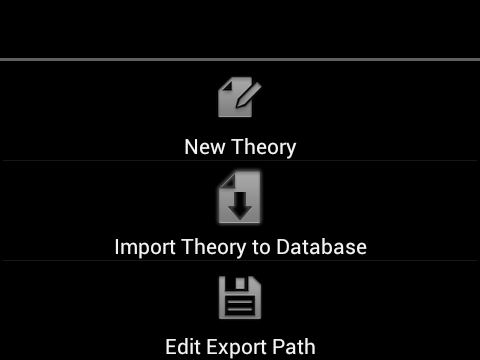
\includegraphics[width=150px]{images/android4.png}
  \caption{Theory database (left) and context menu (right)}\label{fig:android34}
\end{figure}

\begin{figure}
\centering
  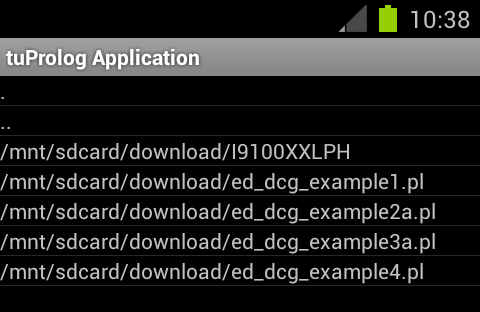
\includegraphics[width=150px]{images/android6.png}
  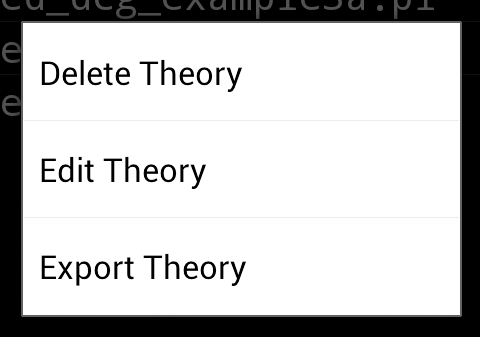
\includegraphics[width=150px]{images/android5.png}
  \caption{Browsing theories (left) and theory operations (right)}\label{fig:android56}
\end{figure}

\begin{figure}
\centering
  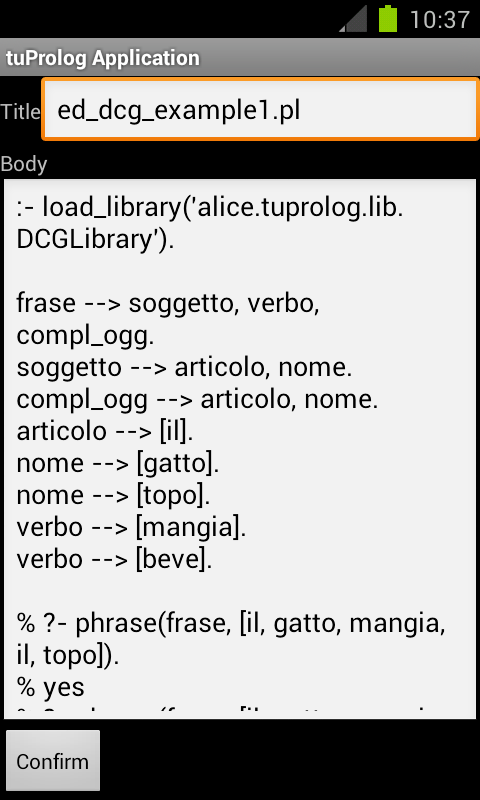
\includegraphics[width=150px]{images/android7.png}
  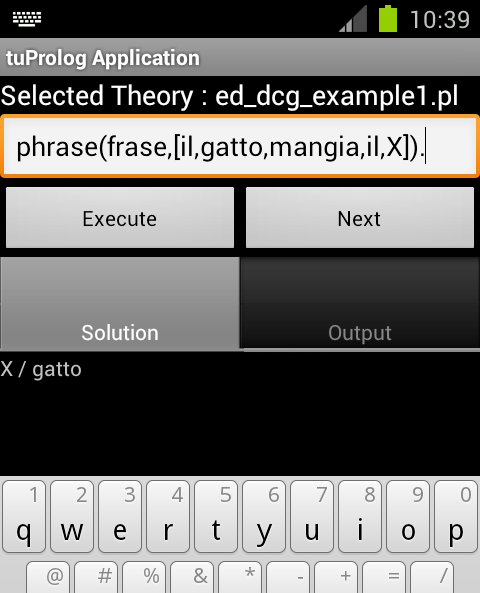
\includegraphics[width=150px]{images/android8.png}
  \caption{Theory editing (left) and query execution (right)}\label{fig:android78}
\end{figure}

Theories in the database can be deleted, edited and exported in a (long-)click, using the proper the context menu item (Figure \ref{fig:android56}, right). The export path can be changed via the \textit{Edit Export Path} in the activity menu.

Editing (Figure \ref{fig:android78}, left) applies both to existing (loaded) files and to brand new theories: to create a new theory, just click on \textit{New Theory} option in the context menu.
%
After editing, to make your changes permanent, the modified theory must be saved to the theory database by clicking the \textit{Confirm} button: alternatively, the back button discards changes.

When a valid theory is loaded, a query can be written in the input field (Figure \ref{fig:android78}, right): an auto-complete mechanism is available which exploits the previous queries to speed up the typing process.
%
Pressing \textit{Execute}, the query solution is shown in the \textit{Solution} tab, along with variable bindings; any output performed by the application is available in the \textit{Output} tab. If multiple solutions exist, the \textit{Next} button is enabled and can be exploited to browse them---the corresponding output being shown in the \textit{Output} tab.

Finally, if the query performs an operation requiring an input from the standard input stream (e.g. via some of the IOLibrary/ISOIOLibrary input predicates, like \texttt{read}), the app intercepts the request and shows the corresponding dialog (Figure \ref{fig:android9}): this feature is available since \tuprolog{} 2.8.
More on this in Section \ref{sec:io-library}.

\begin{figure}
\centering
  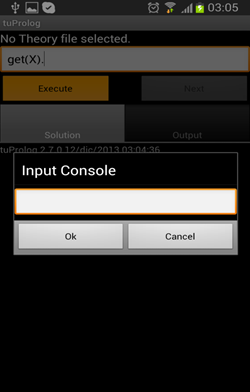
\includegraphics[width=150px]{images/android-inputFromConsole.png}
  \caption{Keyboard input management in the case of a read operation from the standard input.}\label{fig:android9}
\end{figure}

%******************************************************************************%
%=======================================================================
\chapter{\tuprolog{} Basics}
\label{ch:engine}
%=======================================================================

This chapter overviews the basic elements and structure of the \tuprolog{} engine, the \tuprolog{} syntax, the programming support, and the built-in predicates.
%
Additional predicates, provided by libraries, are presented in the next Chapter.

%---------------------------------------------------------------------
\section{Predicate categories}
\label{sec:predicate-categories}
%---------------------------------------------------------------------

In \tuprolog{}, predicates are organized into three different categories:
%
\begin{description}
\item[built-in predicates] |
Built-in predicates are so-called because they are defined at the \tuprolog{} core level. They constitute a small but essential set of predicates, that any \tuprolog{} engine can count on.
%
Any modification possibly made to the engine before or during execution will never affect the number and properties of these predicates.


\item[library predicates] |
Predicates loaded in a \tuprolog{} engine by means of a \tuprolog{} library are called library predicates.
%
Since libraries can be loaded and unloaded in \tuprolog{} engines freely at the system start-up, or dynamically at run time, the set of the library predicates of a \tuprolog{} engine is not fixed, and can change from engine to engine, as well as at different times for the same engine.
%
It is worth noting that library predicates cannot be individually retracted: to remove an undesired library predicate from the engine, the whole library containing that predicate needs to be unloaded.
%
%As discussed in Chapter \ref{ch:howto-develop-libraries}, \tuprolog{} libraries can be implemented mixing Java and Prolog code.

Library predicates can be overridden by theory predicates, that is, predicates defined in the user theory.


\item[theory predicates] |
Predicates loaded in a \tuprolog{} engine by means of a \tuprolog{} theory are called theory predicates.
%
Since theories can be loaded and unloaded in \tuprolog{} engines freely at the system start-up, or dynamically at execution time, the set of the theory predicates of a \tuprolog{} engine is not fixed, and can change from engine to engine, as well as at different times for the same engine.
%
%\tuprolog{} theories are collections of Prolog clauses.
\end{description}


It is worth highlighting that, though they may seem similar, library and theory predicates are not the same, and are handled differently by the \tuprolog{} engine.
%
The difference between the two categories is both \textit{conceptual} and \textit{structural}.

Conceptually speaking, theory predicates should be used to axiomatically represent domain knowledge at the time the proof is performed, while library predicates should be used to represent what is required (procedural knowledge, utility predicates) in order to actually and effectively perform proofs in the domain of interest. So, from this viewpoint, library predicates are devoted to represent more ``stable'' knowledge than theory predicates.
%
Correspondingly, library and theory predicates are represented differently at run-time, and are handled differently by the engine---in particular, with respect to the observation level for monitoring and debugging purposes.
%
In particular, library predicates are usually step over during debugging, coherently with their more stable (and expectedly well-tested) nature, while theory predicates are step into in a detailed way during the controlled execution.
%
This is also why all the tools in the \tuprolog{} GUI show in a separate way the theory predicates, on the one hand, and the loaded libraries and predicates, on the other.


%---------------------------------------------------------------------
\section{Syntax}
\label{sec:syntax}
%---------------------------------------------------------------------

The term syntax supported by \tuprolog{} engine is basically ISO compliant,\footnote{Some ISO directives, however, are not supported.} and accounts for several elements:
%
\begin{description}

\item[Atoms] |
There are four types of atoms:
\emph{(i)} a series of letters, digit, and/or underscores, beginning with a lower-case letter; \emph{(ii)} a series of one or more characters from the set \{\texttt{\#}, \texttt{\$}, \texttt{\&}, \texttt{*}, \texttt{+}, \texttt{-}, \texttt{.}, \texttt{/}, \texttt{:}, \texttt{<}, \texttt{=}, \texttt{>}, \texttt{?}, \texttt{@}, \texttt{\textasciicircum}, \texttt{\~}\}, provided it does not begin with \texttt{/*};
\emph{(iii)} The special atoms \texttt{[]} and \texttt{\{\}};
\emph{(iv)} a single-quoted string.

\item[Variables] |
A variable name begins with a capital
letter or the underscore mark (\bt{\_}), and consists of letters,
digits, and/or underscores.
%
A single underscore mark denotes an anonymous variable.

\item[Numbers] |
Integers and float are supported.
%
The formats supported for integer numbers are decimal, binary (with \verb|0b|
prefix), octal (with \verb|0o| prefix), and hexadecimal (with \verb|0x|
prefix). The character code format for integer numbers (prefixed by \verb|0'|) is supported only for alphanumeric characters, the white space, and characters in the set \{\texttt{\#}, \texttt{\$}, \texttt{\&}, \texttt{*}, \texttt{+}, \texttt{-}, \texttt{.}, \texttt{/}, \texttt{:}, \texttt{<}, \texttt{=}, \texttt{>}, \texttt{?}, \texttt{@}, \texttt{\textasciicircum}, \texttt{\~}\}.
%
The range of integers is -2147483648 to 2147483647; the range of floats is
-2E+63 to 2E+63-1.
%
Floating point numbers can be expressed also in the exponential format (e.g. \bt{-3.03E-05}, \bt{0.303E+13}).
%
A minus can be written before any number to make it negative (e.g. \bt{-3.03}).
%
Notice that the minus is the sign-part of the number itself; hence \bt{-3.4} is a number, not an expression (by contrast, \bt{- 3.4} is an expression).

\item[Strings] |
A series of ASCII characters, embedded in quotes \verb|'| or \verb|"|.
%
Within single quotes, a single quote is written double (e.g, \verb|'don''t forget'|).
%
A backslash at the very end of the line denotes continuation to the next line, so that: \\
\verb|'this is \ |\\
\verb|a single line'|\\
is equivalent to \verb|'this is a single line'| (the line break is ignored).
%
Within a string, the backslash can be used to denote special characters, such as \verb|\n| for a newline,
\verb|\r| for a return without newline,
\verb|\t| for a tab character,
\verb|\\| for a backslash,
\verb|\'| for a single quote,
\verb|\"| for a double quote.

\item[Compounds] |
The ordinary way to write a compound is to write the functor (as an atom), an opening parenthesis, without spaces between them, and then a series of terms separated by commas, and a closing parenthesis: \bt{f(a,b,c)}.
%
This notation can be used also for functors that are normally written as operators, e.g. \bt{2+2} = \verb|'+'(2,2)|.
%
Lists are defined as rightward-nested structures using the dot operator \verb|'.'|; so, for example: \\
\bt{[a] =} \verb|'.'(a,[])|\\
\bt{[a,b] =} \verb|'.'(a,'.'(b,[]))|\\
\bt{[a,b|c] =} \verb|'.'(a,'.'(b,c))|\\
%
There can be only one \bt{|} in a list, and no commas after it.
%
Also curly brackets are supported: any term enclosed with \bt{$\{$} and \bt{$\}$} is treated as the argument of the special functor \verb|'{}'|:  \verb|{hotel}| = \verb|'{}'(hotel)|, \bt{$\{$1,2,3$\}$} = \verb|'{}'(1,2,3)|.
%
Curly brackets can be used in the Definite Clause Grammars theory.


\item[Comments and Whitespaces] -- Whitespaces consist of blanks (including tabs and formfeeds), end-of-line marks, and comments. A whitespace can be put before and after any term, operator, bracket, or argument separator, as long as it does not break up an atom or number or separate a functor from the opening parenthesis that introduces its argument lists.
%
For instance, atom \bt{p(a,b,c)} can be written as \bt{p(\mbox{~a~},\mbox{~b~},\mbox{~c~})}, but not as \bt{\mbox{p~}(a,b,c)}).
%
Two types of comments are supported: one type begins with \bt{/*} and ends with \bt{*/}, the other begins with \bt{\%} and ends at the end of the line.
%
Nested comments are not allowed.


\item[Operators] |
Operators are characterised by a name, a specifier, and a priority.
%
An operator name is an atom, which is not univocal: the same atom can be an operator in more than one class, as in the case of the infix and prefix minus signs.
%
An operator  specifier is a string like \texttt{xfy}, which gives both its class (infix, postfix and prefix) and its associativity: \texttt{xfy} specifies that the grouping on the right should be formed first, \texttt{yfx} on the left, \texttt{xfx} no priority.
%
An operator priority is a non-negative integer ranging from 0 (max priority) and 1200 (min priority).

Operators can be defined by means of either the \bt{op/3} predicate or directive.
%
No predefined operators are directly given by the raw \tuprolog{} engine, whereas a number of them is provided through libraries.

\item[Commas] |
The comma has three functions: it separates arguments of functors, it separates elements of lists, and it is an infix operator of priority 1000.
%
Thus \bt{(a,b)} (without a functor in front) is a compound, equivalent to \verb|','(a,b)|.

\item[Parentheses] -- Parentheses are allowed around any term.
%
The effect of parentheses is to override any grouping that may
otherwise be imposed by operator priorities.
%
Operators enclosed in parentheses do not work as operators;
thus \bt{2(+)3} is a syntax error.
\end{description}

%---------------------------------------------------------------------
\section{Engine configurability}
\label{sec:engine-configurability}
%---------------------------------------------------------------------
\tuprolog{} engines provides four levels of configurability:

\begin{description}

\item[Libraries] |
At the first level, each \tuprolog{} engine can be dynamically extended by loading or unloading libraries.
%
Each library can provide a specific set of predicates, functors, and a related theory, which also allows new flags and operators to be defined.
%
Libraries can be either pre-defined (see Chapter \ref{ch:standard-libraries}) or user-defined (see Section \ref{sec:howto-develop-libraries}).
%
A library can be loaded by means of the predicate \texttt{load\_library} (Prolog side), or by means of the method \texttt{loadLibrary} of the \tuprolog{} engine (Java/.NET side).


\item[Directives] |
At the second level, directives can be given by means of the \bt{:-/1} predicate, which is natively supported by the engine, and can be used to configure and use a \tuprolog{} engine (\bt{set\_prolog\_flag/1}, \bt{load\_library/1}, \bt{consult/1}, \bt{solve/1}), format and syntax of read-terms\footnote{As specified by the ISO standard, a read-term is a Prolog term followed by an end token, composed by an optional layout text sequence and a dot.} (\bt{op/3}).
%
Directives are described in detail in the following sections.

\item[Flags] |
At the third level, \tuprolog{} supports the dynamic definition of flags to describe relevant aspects of libraries, predicates and evaluable functors.
%
A flag is identified by a name (an alphanumeric atom), a list of possible values, a default value, and a boolean value specifying if the flag value can be modified.
%
Dynamically, a flag value can be changed (if modifiable) with a new value included in the list of possible values.

\item[Theories] |
The fourth level of configurability is given by theories: a theory is a text consisting of a sequence of clauses and/or directives.
%
Clauses and directives are terminated by a dot, and are separated by a whitespace character.
%
Theories can be loaded or unloaded by means of suitable library predicates, which are described in Chapter \ref{ch:standard-libraries}.

\end{description}

%---------------------------------------------------------------------
\section{Exception support}
\label{sec:exception-support}
%---------------------------------------------------------------------

As of version 2.2, \tuprolog{} supports exceptions according to the ISO Prolog standard (ISO/IEC 13211-1) published in 1995.
%
Details about the exception handling mechanism are provided in Chapter \ref{ch:exceptions}: this short overview is functional to the understanding of the built-in predicate specification presented in the next Section.

According to the ISO specification, an \textit{error} is a particular circumstance that interrupts the execution of a Prolog program: when a Prolog engine encounters an error, it raises an \textit{exception}, which is supposed to transfer the execution flow to a suitable exception handler, exiting atomically from any number of nested execution contexts.

%-----------------------------------------------------------------------
\subsection{Error classification}
\label{ssec:error classification}
%-----------------------------------------------------------------------
When an exception is raised, the relevant error information is also transferred by instantiating a suitable \textit{error term}.

The ISO Prolog standard prescribes that such a term follows the pattern
\texttt{error(\textit{Error\_term}, \textit{Implementation\_defined\_term})} where
\texttt{\textit{Error\_term}} is constrained by the standard to a pre-defined set of values (the error categories), and \texttt{\textit{Implementation\_defined\_term}} is an optional term providing implementation-specific details.
%
Ten error categories are defined:
\begin{enumerate}
  \item \texttt{instantiation\_error}: when the argument of a predicate or one of its components is an unbound variable, which should have been instantiated. Example: \texttt{X is Y+1} when \texttt{Y} is not instantiated at the time \texttt{is/2} is evaluated.

  \item \texttt{type\_error(\textit{ValidType}, \textit{Culprit})}: when the type of an argument of a predicate, or one of its components, is instantiated, but is bound to the wrong type of data. \texttt{\textit{ValidType}} represents the expected data type (one of \texttt{atom}, \texttt{atomic}, \texttt{byte}, \texttt{callable}, \texttt{character}, \texttt{evaluable}, \texttt{in\_byte}, \texttt{in\_character}, \texttt{integer}, \texttt{list}, \texttt{number}, \texttt{predicate\_indicator}, \texttt{variable}), and \texttt{\textit{Culprit}} is the actual (wrong) type found.
      Example: a predicate expecting months to be represented as integers in the range 1--12 called with an argument like \texttt{march} instead of \texttt{3}.

  \item \texttt{domain\_error(\textit{ValidDomain}, \textit{Culprit})}: when the argument type is correct, but its value falls outside the expected range.
      \texttt{\textit{ValidDomain}} is one of \texttt{character\_code\_list},
      \texttt{not\_empty\_list}, \texttt{not\_less\_than\_zero}, \texttt{close\_option}, \texttt{io\_mode}, \texttt{operator\_priority}, \texttt{operator\_specifier}, \texttt{flag\_value}, \texttt{prolog\_flag}, \texttt{read\_option}, \texttt{write\_option}, \texttt{source\_sink}, \texttt{stream}, \texttt{stream\_option}, \texttt{stream\_or\_alias}, \texttt{stream\_position},\\
      \texttt{stream\_property}. Example: a predicate expecting months as above, called with an out-of-range argument like \texttt{13}.

  \item \texttt{existence\_error(\textit{ObjectType}, \textit{ObjectName}}): when the referenced object does not exist. \texttt{\textit{ObjectType}} is
      the type of the unexisting object (one of \texttt{procedure}, \texttt{source\_sink}, or \texttt{stream}), and \texttt{\textit{ObjectName}} is the missing object's name. Example: trying to access an unexisting file like \texttt{usr/goofy} leads to an
      \texttt{existence\_error(stream, 'usr/goofy')}.

  \item \texttt{permission\_error(\textit{Operation}, \textit{ObjectType}, \textit{Object})}: whenever\\
       \texttt{\textit{Operation}} (one of \texttt{access}, \texttt{create}, \texttt{input}, \texttt{modify}, \texttt{open}, \texttt{output}, or \texttt{reposition}) is not allowed on \texttt{\textit{Object}}, of type \texttt{\textit{ObjectType}} (one of  \texttt{binary\_stream}, \texttt{past\_end\_of\_stream}, \texttt{operator}, \texttt{private\_procedure}, \texttt{static\_procedure}, \texttt{source\_sink}, \texttt{stream}, \texttt{text\_stream}, \texttt{flag}).

  \item \texttt{representation\_error(\textit{Flag})}: when an implementation-defined limit, whose category is given by \texttt{\textit{Flag}} (one of
      \texttt{character}, \texttt{character\_code}, \texttt{in\_character\_code}, \texttt{max\_arity}, \texttt{max\_integer}, \texttt{min\_integer}), is violated during execution.

  \item \texttt{evaluation\_error(\textit{Error})}: when the evaluation of a function produces an out-of-range value (one of \texttt{float\_overflow}, \texttt{int\_overflow}, \texttt{undefined}, \texttt{underflow}, \texttt{zero\_divisor}).

  \item \texttt{resource\_error(\textit{Resource})}: when the Prolog engine does not have enough resources to complete the execution of the goal. \texttt{Resource} can be any term useful to describe the situation. Examples: maximum number of opened files reached, no further available memory, etc.

  \item \texttt{syntax\_error(\textit{Message})}: when data read from an external source have an incorrect format or cannot be processed for some reason. \texttt{\textit{Message}} can be any term useful to describe the situation.

  \item \texttt{system\_error}: any other unexpected error not falling into the previous categories.
\end{enumerate}


%---------------------------------------------------------------------
\section{Built-in predicates}
\label{sec:builtins}
%---------------------------------------------------------------------

This section contains a comprehensive list of the built-in predicates, that is the predicated defined directly in the \tuprolog{} core, both for efficiency reasons and because they directly affect the resolution process.

Following an established convention, the symbol \bt{+} in front of an argument means an \emph{input argument}, \bt{-} means \emph{output argument}, \bt{?} means \emph{input/output} argument, \bt{@} means \emph{input argument} that must be bound.

%---------------------------------------------------------------------
\subsection{Control management}
\label{ssec:control-management}
%---------------------------------------------------------------------

\begin{itemize}

\item \bti{true/0}\\
    \noindent\bt{true} is true.

\item \bti{fail/0}\\
    \noindent\bt{fail} is false.

\item \verb|','/2|\\
    \noindent\verb|','(First,Second)| is true if and only if both \bt{First}
    and \bt{Second} are true.

\item \bti{!/0}\\
    \noindent\bt{!} is true. All choice points between the cut and the
    parent goal are removed. The effect is a commitment to use both the
    current clause and the substitutions found at the point of the
    cut.

\item \verb|'$call'/1|\\
    \noindent\verb|'$call'(Goal)| is true if and only if \bt{Goal}
    represents a true goal. It is not opaque to cut.

    \template{'\$call'(+callable\_term)}

    \exception{error(instantiation\_error, instantiation\_error(\\
    Goal, ArgNo))} when \texttt{G} is a variable. \texttt{Goal} is the goal where the problem occurred, \texttt{ArgNo} indicates the argument that caused the problem (obviously, \texttt{1}).

    \exception{error(type\_error(ValidType, Culprit), type\_error(\\
    Goal, ArgNo, ValidType, Culprit))} when \texttt{G} is not a callable goal. \texttt{Goal} is the goal where the problem occurred, \texttt{ArgNo} indicates the argument that caused the problem (obviously, \texttt{1}), \texttt{ValidType} is the data type expected for \texttt{G} (here, \texttt{callable}), while \texttt{Culprit} is the actual data type found.

\item \bti{halt/0}\\
    \noindent\bt{halt} terminates a Prolog demonstration, exiting the
    Prolog thread and returning to the parent system. In any of the \tuprolog{} user interfaces -- the GUI, the character-based console, the Android app, the Eclipse plugin -- the effect is to terminate the whole application (including Eclipse itself).

\item \bti{halt/1}\\
    \noindent\bt{halt(X)} terminates a Prolog demonstration, exiting the
    Prolog thread and returning the provided int value to the parent system.
    In any of the \tuprolog{} user interfaces -- the GUI, the character-based console, the Android app, the Eclipse plugin -- the effect is to terminate the whole application (including Eclipse itself).

    \template{halt(+int)}

    \exception{error(instantiation\_error, instantiation\_error(\\
    Goal, ArgNo))} when \texttt{X} is a variable. \texttt{Goal} is the goal where the problem occurred, \texttt{ArgNo} indicates the argument that caused the problem (obviously, \texttt{1}).

    \exception{error(type\_error(ValidType, Culprit), type\_error(\\
    Goal, ArgNo, ValidType, Culprit))} when \texttt{X} is not an integer number. \texttt{Goal} is the goal where the problem occurred, \texttt{ArgNo} indicates the argument that caused the problem (obviously, \texttt{1}), \texttt{ValidType} is the data type expected for \texttt{X} (here, \texttt{integer}), while \texttt{Culprit} is the actual data type found.

\end{itemize}

%---------------------------------------------------------------------
\subsection{Term unification and management}
\label{ssec:term-unification-and-management}
%---------------------------------------------------------------------

\begin{itemize}

\item \bti{is/2}\\
    \noindent\bt{is(X, Y)} is true iff \bt{X} is unifiable with the value of the expression \bt{Y}.

    \template{is(?term, @evaluable)}

    \exception{error(instantiation\_error, instantiation\_error(\\
    Goal, ArgNo))} when \texttt{Y} is a variable. \texttt{Goal} is the goal where the problem occurred, \texttt{ArgNo} indicates the argument that caused the problem (here, \texttt{2}).

    \exception{error(type\_error(ValidType, Culprit), type\_error(\\
    Goal, ArgNo, ValidType, Culprit))} when \texttt{Y} is not a valid expression. \texttt{Goal} is the goal where the problem occurred, \texttt{ArgNo} indicates the argument that caused the problem (clearly, \texttt{2}), \texttt{ValidType} is the data type expected for \texttt{G} (here, \texttt{evaluable}), while \texttt{Culprit} is the actual data type found.

    \exception{error(evaluation\_error (Error), evaluation\_error(\\
    Goal, ArgNo, Error))} when an error occurs during the evaluation of \texttt{Y}. \texttt{Goal} is the goal where the problem occurred, \texttt{ArgNo} indicates the argument that caused the problem (clearly, \texttt{2}), and \texttt{Error} is the error occurred (e.g. \texttt{zero\_division} in case of a division by zero).

\item \verb|'='/2|\\
    \noindent\verb|'='(X, Y)| is true iff \bt{X} and \bt{Y} are unifiable.

    \template{'='(?term, ?term)}

\item \verb|'\='/2|\\
    \noindent\verb|'\='(X, Y)| is true iff \bt{X} and \bt{Y} are not unifiable.

    \template{'$\setminus$='(?term, ?term)}

\item \verb|'$tolist'/2|\\
    \noindent\verb|'$tolist'(Compound, List)| is true if \bt{Compound} is a compound term, and in this case \bt{List} is list representation of the compound, with the name as first element and all the arguments as other elements.

    \template{'\$tolist'(@struct, -list)}

    \exception{error(instantiation\_error, instantiation\_error(\\
    Goal, ArgNo))} when \texttt{Struct} is a variable. \texttt{Goal} is the goal where the problem occurred, \texttt{ArgNo} indicates the argument that caused the problem (obviously, \texttt{1}).

    \exception{error(type\_error(ValidType, Culprit), type\_error(\\
    Goal, ArgNo, ValidType, Culprit))} when \texttt{Struct} is not a structure. \texttt{Goal} is the goal where the problem occurred, \texttt{ArgNo} indicates the argument that caused the problem (clearly, \texttt{1}), \texttt{ValidType} is the data type expected for \texttt{G} (here, \texttt{struct}), while \texttt{Culprit} is the actual data type found.

\item \verb|'$fromlist'/2|\\
    \noindent\verb|'$fromlist'(Compound, List)| is true if \bt{Compound} unifies with the list representation of \bt{List}.

    \template{'\$fromlist'(-struct, @list)}

    \exception{error(instantiation\_error, instantiation\_error(\\
    Goal, ArgNo))} when \texttt{List} is a variable. \texttt{Goal} is the goal where the problem occurred, \texttt{ArgNo} indicates the argument that caused the problem (obviously, \texttt{2}).

    \exception{error(type\_error(ValidType, Culprit), type\_error(\\
    Goal, ArgNo, ValidType, Culprit))} when \texttt{List} is not a list. \texttt{Goal} is the goal where the problem occurred, \texttt{ArgNo} indicates the argument that caused the problem (clearly, \texttt{2}), \texttt{ValidType} is the data type expected for \texttt{G} (here, \texttt{list}), while \texttt{Culprit} is the actual data type found.

\item \bti{copy\_term/2}\\
    \noindent\bt{copy\_term(Term1, Term2)} is true iff \bt{Term2} unifies with the a renamed copy of \bt{Term1}.

    \template{copy\_term(?term, ?term)}

\item \verb|'$append'/2|\\
    \noindent\verb|'$append'(Element, List)| is true if \bt{List} is a list, with the side effect that the \bt{Element} is appended to the list.

    \template{'\$append'(+term, @list)}

    \exception{error(instantiation\_error, instantiation\_error(\\
    Goal, ArgNo))} when \texttt{List} is a variable. \texttt{Goal} is the goal where the problem occurred, \texttt{ArgNo} indicates the argument that caused the problem (obviously, \texttt{2}).

    \exception{error(type\_error(ValidType, Culprit), type\_error(\\
    Goal, ArgNo, ValidType, Culprit))} when \texttt{List} is not a list. \texttt{Goal} is the goal where the problem occurred, \texttt{ArgNo} indicates the argument that caused the problem (clearly, \texttt{2}), \texttt{ValidType} is the data type expected for \texttt{G} (here, \texttt{list}), while \texttt{Culprit} is the actual data type found.

\end{itemize}

%---------------------------------------------------------------------
\subsection{Knowledge base management}
\label{ssec:knowledge-base-management}
%---------------------------------------------------------------------

\begin{itemize}

\item
    \verb|'$find'/2|\\
    \noindent\verb|'$find'(Clause, Clauses)| is true if \bt{Clause} is a clause and \bt{Clauses} is a list: as a side effect, all the database clauses matching \bt{Clause} are appended to the \bt{Clauses} list.

    \template{'\$find'(@clause, @list)}

    \exception{error(instantiation\_error, instantiation\_error(\\
    Goal, ArgNo))} when \texttt{Clause} is a variable. \texttt{Goal} is the goal where the problem occurred, \texttt{ArgNo} indicates the argument that caused the problem (here, \texttt{1}).

    \exception{error(type\_error(ValidType, Culprit), type\_error(\\
    Goal, ArgNo, ValidType, Culprit))} when \texttt{Clauses} is not a list. \texttt{Goal} is the goal where the problem occurred, \texttt{ArgNo} indicates the argument that caused the problem (here, \texttt{2}), \texttt{ValidType} is the data type expected for \texttt{Clauses} (i.e. \texttt{list}), while \texttt{Culprit} is the actual data type found.

\item
    \bti{abolish/1}\\
    \noindent\bt{abolish(Predicate)} completely wipes out the dynamic
    predicate matching \texttt{Predicate}.

    \template{\bt{abolish(@term)}}

    \exception{error(instantiation\_error, instantiation\_error(\\
    Goal, ArgNo))} when \texttt{Predicate} is a variable. \texttt{Goal} is the goal where the problem occurred, \texttt{ArgNo} indicates the argument that caused the problem (obviously, \texttt{1}).

    \exception{error(type\_error(ValidType, Culprit), type\_error(\\
    Goal, ArgNo, ValidType, Culprit))} when \texttt{Predicate} is not a structure. \texttt{Goal} is the goal where the problem occurred, \texttt{ArgNo} indicates the argument that caused the problem (obviously, \texttt{1}), \texttt{ValidType} is the data type expected for \texttt{Predicate}, while \texttt{Culprit} is the actual data type found.

\item \bti{asserta/1}\\
    \noindent\bt{asserta(Clause)} is true, with the side effect that
    the clause \bt{Clause} is added to the beginning of database.

    \template{asserta(@clause)}

    \exception{error(instantiation\_error, instantiation\_error(\\
    Goal, ArgNo))} when \texttt{Clause} is a variable. \texttt{Goal} is the goal where the problem occurred, \texttt{ArgNo} indicates the argument that caused the problem (obviously, \texttt{1}).

    \exception{error(type\_error(ValidType, Culprit), type\_error(\\
    Goal, ArgNo, ValidType, Culprit))} when \texttt{Clause} is not a structure. \texttt{Goal} is the goal where the problem occurred, \texttt{ArgNo} indicates the argument that caused the problem (obviously, \texttt{1}), \texttt{ValidType} is the data type expected for \texttt{Clause}, while \texttt{Culprit} is the actual data type found.

\item \bti{assertz/1}\\
    \noindent\bt{assertz(Clause)} is true, with the side effect that
    the clause \bt{Clause} is added to the end of the database.

    \template{assertz(@clause)}

    \exception{error(instantiation\_error, instantiation\_error(\\
    Goal, ArgNo))} when \texttt{Clause} is a variable. \texttt{Goal} is the goal where the problem occurred, \texttt{ArgNo} indicates the argument that caused the problem (obviously, \texttt{1}).

    \exception{error(type\_error(ValidType, Culprit), type\_error(\\
    Goal, ArgNo, ValidType, Culprit))} when \texttt{Clause} is not a structure. \texttt{Goal} is the goal where the problem occurred, \texttt{ArgNo} indicates the argument that caused the problem (obviously, \texttt{1}), \texttt{ValidType} is the data type expected for \texttt{Clause}, while \texttt{Culprit} is the actual data type found.

\item \verb|'$retract'/1|\\
    \noindent\verb|'$retract'(Clause)| is true if the database contains
    at least one clause unifying with \bt{Clause}; as a side effect, the
    clause is removed from the database. It is not re-executable.
    Please do not confuse this built-in predicate with the \texttt{retract/1} predicate of \textit{BasicLibrary}.

    \template{'\$retract'(@clause)}

    \exception{error(instantiation\_error, instantiation\_error(\\
    Goal, ArgNo))} when \texttt{Clause} is a variable. \texttt{Goal} is the goal where the problem occurred, \texttt{ArgNo} indicates the argument that caused the problem (obviously, \texttt{1}).

    \exception{error(type\_error(ValidType, Culprit), type\_error(\\
    Goal, ArgNo, ValidType, Culprit))} when \texttt{Clause} is not a structure. \texttt{Goal} is the goal where the problem occurred, \texttt{ArgNo} indicates the argument that caused the problem (obviously, \texttt{1}), \texttt{ValidType} is the data type expected for \texttt{Clause}, while \texttt{Culprit} is the actual data type found.

\end{itemize}

%---------------------------------------------------------------------
\subsection{Operator and flag management}
\label{ssec:operator-and-flag-management}
%---------------------------------------------------------------------

\begin{itemize}

\item \bti{op/3}\\
    \noindent\bt{op(Priority, Specifier, Operator)} is true. It always succeeds,
    modifying the operator table as a side effect. If \bt{Priority} is 0, then
    \bt{Operator} is removed from the operator table; else, \bt{Operator} is
    added to the operator table, with priority (lower binds tighter) \bt{Priority}
    and associativity determined by \bt{Specifier}. If an operator with the same
    \bt{Operator} symbol and the same \bt{Specifier} already exists in the operator
    table, the predicate modifies its priority according to the specified \bt{Priority} argument.

    \template{op(+integer, +specifier, @atom\_or\_atom\_list)}

 \item \bti{flag\_list/1}\\
     \noindent\bt{flag\_list(FlagList)} is true and \bt{FlagList} is the list of the flags currently defined in the engine.

     \template{flag\_list(-list)}

\item \bti{set\_prolog\_flag/2}\\
    \noindent\bt{set\_prolog\_flag(Flag, Value)} is true, and as a side effect associates \bt{Value} with the flag \bt{Flag}, where \bt{Value} is a value that is within the implementation defined range of values for \bt{Flag}.

    \template{set\_prolog\_flag(+flag, @nonvar)}

    \exception{error(instantiation\_error, instantiation\_error(\\
    Goal, ArgNo))} if either \texttt{Flag} or \texttt{Value} is a variable. \texttt{Goal} is the goal where the problem occurred, \texttt{ArgNo} indicates the argument that caused the problem (\texttt{1} or \texttt{2}).

    \exception{error(type\_error(ValidType, Culprit), type\_error(\\
    Goal, ArgNo, ValidType, Culprit))} if \texttt{Flag} is not a structure or \texttt{Value} is not ground. \texttt{Goal} is the goal where the problem occurred, \texttt{ArgNo} indicates the argument that caused the problem (\texttt{1} or \texttt{2}), \texttt{Valid-}\\\texttt{Type} is the data type expected for \texttt{Flag} or \texttt{Value} (\texttt{struct} or \texttt{ground}, respectively), while \texttt{Culprit} is the actual wrong term (either \texttt{Flag} or \texttt{Value}).

    \exception{error(domain\_error(ValidDomain, Culprit), domain\_\\error(Goal, ArgNo, ValidDomain, Culprit))} if \texttt{Flag} is undefined in the engine or \texttt{Value} is not admissible for \texttt{Flag}. \texttt{Goal} is the goal where the problem occurred, \texttt{ArgNo} indicates the argument that caused the problem (\texttt{1} or \texttt{2}), \texttt{ValidDomain} is the data type expected for \texttt{Flag} or \texttt{Value} (\texttt{prolog\_flag} or \texttt{flag\_value}, respectively), while \texttt{Culprit} is the actual wrong term (either \texttt{Flag} or \texttt{Value}).

    \exception{error(permission\_error(Operation, ObjectType,\\Culprit), permission\_error(Goal, Operation, ObjectType,\\Culprit, Message))} if \texttt{Flag} is unmodifiable. \texttt{Goal} is the goal where the problem occurred, \texttt{Operation} is the operation that caused the problem (\texttt{modify}), \texttt{ObjectType} is the data type of the flag (i.e. \texttt{flag}), \texttt{Culprit} is the actual wrong term (clearly, \texttt{Flag}), and \texttt{Message} adds possible extra info (by convention, the atom \texttt{0} is used when no extra info exists).

\item \bti{get\_prolog\_flag/2}\\
    \noindent\bt{get\_prolog\_flag(Flag, Value)} is true iff \bt{Flag} is a flag supported by the engine and \bt{Value} is the value currently associated with it. It is not re-executable.

    \template{get\_prolog\_flag(+flag, ?term)}

    \exception{error(instantiation\_error, instantiation\_error(\\
    Goal, ArgNo))} when \texttt{Flag} is a variable. \texttt{Goal} is the goal where the problem occurred, \texttt{ArgNo} indicates the argument that caused the problem (obviously, \texttt{1}).

    \exception{error(type\_error(ValidType, Culprit), type\_error(\\
    Goal, ArgNo, ValidType, Culprit))} when \texttt{Flag} is not a structure. \texttt{Goal} is the goal where the problem occurred, \texttt{ArgNo} indicates the argument that caused the problem (clearly, \texttt{1}), \texttt{ValidType} is the data type expected for \texttt{G} (here, \texttt{struct}), while \texttt{Culprit} is the actual data type found.

    \exception{error(domain\_error(ValidDomain, Culprit), domain\_\\error(Goal, ArgNo, ValidDomain, Culprit))} if \texttt{Flag} is undefined in the engine. \texttt{Goal} is the goal where the problem occurred, \texttt{ArgNo} indicates the argument that caused the problem (clearly, \texttt{1}), \texttt{ValidDomain} is the domain expected for \texttt{G} (here, \texttt{prolog\_flag}), while \texttt{Culprit} is the actual wrong term found.

\end{itemize}

%---------------------------------------------------------------------
\subsection{Library management}
\label{ssec:library-management}
%---------------------------------------------------------------------

\begin{itemize}

\item \bti{load\_library/1}\\
    \bt{load\_library(LibraryName)} is true if \bt{LibraryName} is the name of a \tuprolog{} library available for loading. As side effect, the specified library is loaded by the engine. Actually \bt{LibraryName} is the full name of the Java class providing the library.

    \template{load\_library(@string)}

    \exception{error(instantiation\_error, instantiation\_error(\\
    Goal, ArgNo))} when \texttt{LibraryName} is a variable. \texttt{Goal} is the goal where the problem occurred, \texttt{ArgNo} indicates the argument that caused the problem (obviously, \texttt{1}).

    \exception{error(type\_error(ValidType, Culprit), type\_error(\\
    Goal, ArgNo, ValidType, Culprit))} when \texttt{LibraryName} is not an atom. \texttt{Goal} is the goal where the problem occurred, \texttt{ArgNo} indicates the argument that caused the problem (obviously, \texttt{1}), \texttt{ValidType} is the data type expected for \texttt{LibraryName}, while \texttt{Culprit} is the actual data type found.

    \exception{error(existence\_error(ObjectType, Culprit),\\existence\_error(Goal, ArgNo, ObjectType, Culprit, Message))} when the library \texttt{LibraryName} does not exist. \texttt{Goal} is the goal where the problem occurred, \texttt{ArgNo} indicates the argument that caused the problem (obviously, \texttt{1}), \texttt{ObjectType} is the data type expected for the missing object (here, \texttt{class}), while \texttt{Culprit} is the actual data type found and \texttt{Message} provides extra info about the occurred error.

 \item \bti{unload\_library/1}\\
    \noindent\bt{unload\_library(LibraryName)} is true if \bt{LibraryName} is the name of a library currently loaded in the engine. As side effect, the library is unloaded from the engine. Actually \bt{LibraryName} is the full name of the Java class providing the library.

    \template{unload\_library(@string)}

    \exception{error(instantiation\_error, instantiation\_error(\\
    Goal, ArgNo))} when \texttt{LibraryName} is a variable. \texttt{Goal} is the goal where the problem occurred, \texttt{ArgNo} indicates the argument that caused the problem (obviously, \texttt{1}).

    \exception{error(type\_error(ValidType, Culprit), type\_error(\\
    Goal, ArgNo, ValidType, Culprit))} when \texttt{LibraryName} is not an atom. \texttt{Goal} is the goal where the problem occurred, \texttt{ArgNo} indicates the argument that caused the problem (obviously, \texttt{1}), \texttt{ValidType} is the data type expected for \texttt{LibraryName}, while \texttt{Culprit} is the actual data type found.

    \exception{error(existence\_error(ObjectType, Culprit),\\existence\_error(Goal, ArgNo, ObjectType, Culprit, Message))} when the library \texttt{LibraryName} does not exist. \texttt{Goal} is the goal where the problem occurred, \texttt{ArgNo} indicates the argument that caused the problem (obviously, \texttt{1}), \texttt{ObjectType} is the data type expected for the missing object (here, \texttt{class}), while \texttt{Culprit} is the actual data type found and \texttt{Message} provides extra info about the occurred error.

\end{itemize}

%---------------------------------------------------------------------
\subsection{Directives}
\label{ssec:directives}
%---------------------------------------------------------------------

Directives are basically queries immediately executed at the theory load time.
%
Unlike other Prolog systems, \tuprolog{} does not allow directives to be composed---that is, each directive must contain only one query: multiple directives require multiple queries.
%
The standard directives are as follows:

\begin{itemize}

\item \bti{:- op/3}\\
     \noindent\bt{op(Priority, Specifier, Operator)} adds \bt{Operator}
     to the operator table, with priority (lower binds tighter)
     \bt{Priority} and associativity determined by \bt{Specifier}.

     \template{op(+integer, +specifier, @atom\_or\_atom\_list)}

    \exception{error(instantiation\_error, instantiation\_error(\\
    Goal, ArgNo))} if any of \texttt{Priority}, \texttt{Specifier} or \texttt{Operator} is a variable. \texttt{Goal} is the goal where the problem occurred, \texttt{ArgNo} indicates the argument that caused the problem (one of \texttt{1}, \texttt{2}, \texttt{3}).

    \exception{error(type\_error(ValidType, Culprit), type\_error(\\
    Goal, ArgNo, ValidType, Culprit))} if \texttt{Priority} is not an integer number, or \texttt{Specifier} is not an atom, or \texttt{Operator} is not an atom or a list of atoms. \texttt{Goal} is the goal where the problem occurred, \texttt{ArgNo} indicates the argument that caused the problem (one of \texttt{1}, \texttt{2} or \texttt{3}), \texttt{ValidType} is the data type expected for the \texttt{Culprit}, and \texttt{Culprit} is the actual cause of the problem.

    \exception{error(domain\_error(ValidDomain, Culprit), domain\_\\error(Goal, ArgNo, ValidDomain, Culprit))} if the type of \texttt{Priority} and \texttt{Specifier} is correct, but their values are not admissible for the operator priority or associativity, respectively. \texttt{Goal} is the goal where the problem occurred, \texttt{ArgNo} indicates the argument that caused the problem (\texttt{1} or \texttt{2}), \texttt{ValidDomain} is the data type expected for \texttt{Culprit}, and \texttt{Culprit} is the actual wrong term found.

\item \bti{:- flag/4}\\
     \noindent\bt{flag(FlagName, ValidValuesList, DefaultValue, IsModifiable)}
     adds to the engine a new flag, identified by the \bt{FlagName} name, which can assume only the values listed in \bt{ValidValuesList} with \bt{DefaultValue} as default value, and that can be modified if \bt{IsModifiable} is true.

     \template{flag(@string, @list, @term, @{true, false})}

\item \bti{:- initialization/1}\\
     \noindent\bt{initialization(Goal)} sets the starting goal to be executed just
     after the theory has been consulted.

     \template{initialization(@goal)}

\item \bti{:- solve/1}\\
     \noindent Synonym for \bt{initialization/1}. \emph{Deprecated.}

     \template{solve(@goal)}

\item \bti{:- load\_library/1}\\
     The directive version of the \texttt{load\_library/1} predicate documented in Subsection \ref{ssec:library-management}. However, here errors in the library name do not raise exceptions---rather, the directive simply fails, yielding no effect at all.

\item \bti{:- include/1}\\
     \noindent\bt{include(Filename)} immediately loads the theory contained in the file specified by \bt{Filename}. Again, errors in the file name do not raise exceptions: the directive simply fails, yielding no effect at all.

     \template{include(@string)}

\item \bti{:- consult/1}\\
     \noindent Synonym for \bt{include/1}. \emph{Deprecated.}

     \template{consult(@string)}

\end{itemize}

%******************************************************************************%
%=======================================================================
\chapter{\tuprolog{} Libraries}
\label{ch:standard-libraries}
%=======================================================================

Libraries are the means by which \tuprolog{} achieves its
fundamental characteristics of minimality and configurability.
%
The engine is by design choice a minimal, purely-inferential core, which includes only the small set of \emph{built-in}s introduced in the previous Chapter.
%
Any other piece of functionality, in the form of predicates, functors, flags and operators, is delivered by \textit{libraries}, which can be loaded and unloaded to/from the engine at any time: each library can provide a set of predicates, functors and a related theory, which can be used to define new flags and operators.

The dynamic loading of libraries can be exploited, for instance, to bound the availability of some functionalities to a specific use context, as in the following example:
%
\begin{verbatim}
% println/1 is defined in ExampleLibrary
run_test(Test, Result) :- run(Test, Result),
                          load_library('ExampleLibrary'),
                          println(Result),
                          unload_library(ExampleLibrary').
\end{verbatim}
%
%The library name can be different from its fully qualified class name.

\noindent The \tuprolog{} distribution include several standard libraries, some of which are loaded by default into any engine--although it is always possible both to create an engine with no pre-loaded libraries, and to create an engine with different (possibly user-defined or third party) pre-loaded libraries.

The fundamental libraries, loaded by default, are the following:
%
\begin{description}

\item[BasicLibrary] (class \texttt{alice.tuprolog.lib.BasicLibrary}) |
    provides the most common Prolog predicates, functors, and operators.
    In order to separate computation and interaction aspects, no I/O
    predicates are included.

\item[ISOLibrary] (class \texttt{alice.tuprolog.lib.ISOLibrary}) |
    provides predicates and functors that are part of the built-in
    section in the ISO standard \cite{iso95}, and are not provided as
    built-ins or by BasicLibrary.

\item[IOLibrary] (class \texttt{alice.tuprolog.lib.IOLibrary}) |
    provides the classic Prolog I/O predicates, except for the ISO-I/O ones.

\item[JavaLibrary] (class \texttt{alice.tuprolog.lib.JavaLibrary}) |
    provides predicates and functors to support multi-paradigm programming
    between Prolog and Java, enabling a complete yet easy access to the
    object-oriented world of Java from \tuprolog{}: features include the
    creation and access of both existing and new objects, classes,
    and resources.
    In the .NET version of \tuprolog{}, this library is replaced\footnote{%
    Actually, integrated: please see Chapter \ref{ch:mpp-in-dotnet} for details.} by \textbf{OOLibrary}, which extends the multi-paradigm programming approach to virtually any language supported by the .NET platform (Chapter \ref{ch:mpp-in-dotnet}.)

\item[ThreadLibrary] (class \texttt{alice.tuprolog.lib.ThreadLibrary}) |
    provides primitives for explicit multi-thread handling  (new in \tuprolog{} 2.7).

\end{description}

\noindent Other libraries included in the standard \tuprolog{} distribution, but not loaded by default, are the following:

\begin{description}

\item[DCGLibrary] (class \texttt{alice.tuprolog.lib.DCGLibrary}) |
    provides support for Definite Clause Grammar, an extension of context
    free grammars used for describing natural and formal languages.

\item[ISOIOLibrary] (class \texttt{alice.tuprolog.lib.ISOIOLibrary}) |
    extends the above IOLibrary by adding ISO-compliant I/O predicates
    (new in \tuprolog{} 2.6).

\item[SocketLibrary] (class \texttt{alice.tuprolog.lib.SocketLibrary}) |
    provides support for TCP and UDP sockets (new in \tuprolog{} 2.7).
\end{description}

\noindent Further libraries exist that are \textit{not} included in the standard \tuprolog{} distribution, because of their very specific domain: they can be downloaded from the \tuprolog{} site, along with their documentation.
%
Among these, for instance, \texttt{RDFLibrary} (class \texttt{alice.tuprolog.lib.RDFLibrary}) provides predicates and functors to handle RDF documents, etc.

The next Sections present the predicates, functors, operators and flag of each library, as well as the dependencies from other libraries, \textit{except for JavaLibrary}, which is discussed in detail in the context of multi-paradigm programming (Chapter \ref{ch:mpp-in-java}, or Chapter \ref{ch:mpp-in-dotnet} for its counterpart in .NET).
%
Throughout this chapter, \texttt{string} means a single-quoted or double-quoted string, as detailed in Chapter \ref{ch:engine}, while \texttt{expr} means an evaluable expression---that is, a term that can be interpreted as a value by some library functors.

%-----------------------------------------------------------------------
\section{BasicLibrary}
\label{sec:basic-library}
%-----------------------------------------------------------------------

%---------------------------------------------------------------------
\subsection{Predicates}
%---------------------------------------------------------------------

%---------------------------------------------------------------------
\subsubsection{Type Testing}
%---------------------------------------------------------------------

\begin{itemize}
 \item \bti{constant/1}\\
    \noindent\bt{constant(X)} is true iff \bt{X} is a constant value.

    \template{constant(@term)}

 \item \bti{number/1}\\
    \noindent\bt{number(X)} is true iff \bt{X} is an integer or a float.

    \template{number(@term)}

 \item \bti{integer/1}\\
    \noindent\bt{integer(X)} is true iff \bt{X} is an integer.

    \template{integer(@term)}

 \item \bti{float/1}\\
    \noindent\bt{float(X)} is true iff \bt{X} is an float.

    \template{float(@term)}

 \item \bti{atom/1}\\
    \noindent\bt{atom(X)} is true iff \bt{X} is an atom.

    \template{atom(@term)}

 \item \bti{compound/1}\\
    \noindent\bt{compound(X)} is true iff \bt{X} is a compound term, that is neither atomic nor a variable.

    \template{compound(@term)}

 \item \bti{var/1}\\
    \noindent\bt{var(X)} is true iff \bt{X} is a variable.

    \template{var(@term)}

 \item \bti{nonvar/1}\\
    \noindent\bt{nonvar(X)} is true iff \bt{X} is not a variable.

    \template{nonvar(@term)}

 \item \bti{atomic/1}\\
    \noindent\bt{atomic(X)} is true iff \bt{X} is atomic (that is is an atom, an integer or a float).

    \template{atomic(@term)}

 \item \bti{ground/1}\\
    \noindent\bt{ground(X)} is true iff \bt{X} is a ground term.

    \template{ground(@term)}

 \item \bti{list/1}\\
    \noindent\bt{list(X)} is true iff \bt{X} is a list.

    \template{list(@term)}
\end{itemize}

%---------------------------------------------------------------------
\subsubsection{Term Creation, Decomposition and Unification}
%---------------------------------------------------------------------

\begin{itemize}

\item \verb|'=..'/2| : \textit{univ}\\
    \noindent\verb|'=..'(Term, List)| is true if \bt{List} is a list consisting of the functor and all arguments of \bt{Term}, in this order.

    \template{'=..'(?term, ?list)}

\item \bti{functor/3}\\
    \noindent\bt{functor(Term, Functor, Arity)} is true if the term \bt{Term} is a compound term, \bt{Functor} is its functor, and \bt{Arity} (an integer) is its arity; or if \bt{Term} is an atom or number equal to \bt{Functor} and \bt{Arity} is 0.

    \template{functor(?term, ?term, ?integer)}

\item \bti{arg/3}\\
    \noindent\bt{arg(N, Term, Arg)} is true if \bt{Arg} is the \bt{N}th
    arguments of \bt{Term} (counting from 1).

    \template{arg(@integer, @compound, -term)}

    \exception{error(instantiation\_error, instantiation\_error(\\
    Goal, ArgNo))} if \texttt{N} or \texttt{Term} are variables. \texttt{Goal} is the goal where the problem occurred, \texttt{ArgNo} indicates the argument that caused the problem (here, \texttt{1} or \texttt{2}).

    \exception{error(type\_error(ValidType, Culprit), type\_error(\\
    Goal, ArgNo, ValidType, Culprit))} if \texttt{N} is not an integer number or \texttt{Term} is not a compound term. \texttt{Goal} is the goal where the problem occurred, \texttt{ArgNo} indicates the argument that caused the problem (here, \texttt{1} or \texttt{2}), \texttt{ValidType} is the expected data type (\texttt{integer} or \texttt{compound}, respectively), \texttt{Culprit} is the wrong term found (either \texttt{N} or \texttt{Term}).

    \exception{error(domain\_error(ValidDomain, Culprit), domain\_\\
    error(Goal, ArgNo, ValidDomain, Culprit))} if \texttt{N} is an int value less than 1. \texttt{Goal} is the goal where the problem occurred, \texttt{ArgNo} indicates the argument that caused the problem (clearly, \texttt{1}), \texttt{ValidDomain} is the expected domain (\texttt{greater\_than\_zero}, respectively), \texttt{Culprit} is the wrong term found (obviously, \texttt{N}).

\item \bti{text\_term/2}\\
    \noindent\bt{text\_term(Text, Term)} is true iff \bt{Text} is the text representation of the term \bt{Term}.

    \template{text\_term(?text, ?term)}

\item \bti{text\_concat/3}\\
    \noindent\bt{text\_concat(Text1, Text2, TextDest)} is
    true iff \bt{TextDest} is the text resulting by appending the text
    \bt{Text2} to \bt{Text1}.

    \template{text\_concat(@string, @string, -string)}

    \exception{error(instantiation\_error, instantiation\_error(\\
    Goal, ArgNo))} if \texttt{Text1} or \texttt{Text2} are variables. \texttt{Goal} is the goal where the problem occurred, \texttt{ArgNo} indicates the argument that caused the problem (here, \texttt{1} or \texttt{2}).

    \exception{error(type\_error(ValidType, Culprit), type\_error(\\
    Goal, ArgNo, ValidType, Culprit))} if \texttt{Text1} or \texttt{Text2} are not atoms. \texttt{Goal} is the goal where the problem occurred, \texttt{ArgNo} indicates the argument that caused the problem (here, \texttt{1} or \texttt{2}),
    \texttt{ValidType} is the expected data type (e.g. \texttt{atom}), \texttt{Culprit} is the wrong term found (either \texttt{Text1} or \texttt{Text2}).

\item \bti{num\_atom/2}\\
    \noindent\bt{num\_atom(Number, Atom)} succeeds iff \bt{Atom} is the atom representation of the number \bt{Number}

    \template{number\_codes(+number, ?atom)}

    \template{number\_codes(?number, +atom)}

    \exception{error(type\_error(ValidType, Culprit), type\_error(\\
    Goal, ArgNo, ValidType, Culprit))} if \texttt{Atom} is a variable and \texttt{Number} is not a number, or, viceversa, if \texttt{Atom} is not an atom. \texttt{Goal} is the goal where the problem occurred, \texttt{ArgNo} indicates the argument that caused the problem (here, \texttt{1} or \texttt{2}), \texttt{ValidType} is the expected data type for the wrong argument (e.g. either \texttt{number} or \texttt{atom}), \texttt{Culprit} is the wrong term found (either \texttt{Number} or \texttt{Atom}).

    \exception{error(domain\_error(ValidType, Culprit), domain\_\\
    error(Goal, ArgNo, ValidDomain, Culprit))} if \texttt{Atom} is an atom that does not represent a number. \texttt{Goal} is the goal where the problem occurred, \texttt{ArgNo} indicates the argument that caused the problem (clearly, \texttt{2}), \texttt{ValidDomain} is the expected domain for the wrong argument (\texttt{num\_atom}), \texttt{Culprit} is the wrong term found (obviously \texttt{Atom}).

\end{itemize}

%---------------------------------------------------------------------
\subsubsection{Occurs Check}
%---------------------------------------------------------------------

\noindent When the process of unification takes place between a variable $S$ and a term $T$, the first thing a Prolog engine should do before proceeding is to check that $T$ does not contain any occurrences of $S$.
This test is known as \emph{occurs check} \cite{ss94} and is conceptually necessary to prevent the unification of terms such as $s(X)$ and $X$, for which no finite common instance exists; yet, the test implies a performance drawback that impacts on the speed and efficiency of the resolution process.

For this reason, most Prolog implementations omit the occur check from their unification algorithm, providing a specific predicate for ``augmented unification'' (that is, unification including the occurs check), to be used when the programmer wants to stay on the safer side:

\begin{itemize}
\item \bti{unify\_with\_occurs\_check/2}\\
    \noindent\bt{unify\_with\_occurs\_check(X, Y)} is true iff \bt{X} and \bt{Y} are unifiable.

    \template{unify\_with\_occurs\_check(?term, ?term)}

\end{itemize}

\noindent \tuprolog{} is an exception in this panorama, because its unification algorithm \textit{always performs the occurs check}: the \bti{unify\_with\_occurs\_check/2} is supported, but is merely a renaming of the standard \texttt{=/2} unification operator.

As a consequence, goals like \texttt{X=f(X)}, that may loop or be solved in an ``infinite'' form in other Prolog systems\footnote{SICStus Prolog, for instance, succeeds returning a solution like \texttt{X=f(f(f(f(f(f(f(f(f(f(...))))))))))}, where the inner dots ``hide'' the infinite self-substitution.}, are occurs-checked in \tuprolog, leading to a failure.


%---------------------------------------------------------------------
\subsubsection{Expression and Term Comparison}
%---------------------------------------------------------------------
\begin{itemize}
    \item expression comparison (generic template:
    \emph{pred}(@expr, @expr)):\\
        \verb|'=:=', '=\=', '>', '<', '>=', '=<'|;

    \item term comparison (generic template:
    \emph{pred}(@term, @term)):\\
         \verb|'==', '\==', '@>', '@<', '@>=', '@=<'|.
\end{itemize}

%---------------------------------------------------------------------
\subsubsection{Finding Solutions}
%---------------------------------------------------------------------
\begin{itemize}
%
\item \bti{findall/3}\\
    \noindent\bt{findall(Template, Goal, List)} is true if and only if
    \bt{List} unifies with the list of values to which a variable X not
    occurring in \bt{Template} or \bt{Goal} would be instantiated
    by successive re-executions of \bt{call(Goal), X = Template} after systematic replacement of all variables in X by new variables.

    \template{\bt{findall(?term, +callable\_term, ?list)}}

    \exception{error(instantiation\_error, instantiation\_error(\\
    Goal, ArgNo))} if \texttt{G} is a variable. \texttt{Goal} is the goal where the problem occurred, \texttt{ArgNo} indicates the argument that caused the problem (obviously, \texttt{1}).

    \exception{error(type\_error(ValidType, Culprit), type\_error(\\
    Goal, ArgNo, ValidType, Culprit))} if \texttt{G} is not a callable goal (for instance, it is a number). \texttt{Goal} is the goal where the problem occurred, \texttt{ArgNo} indicates the argument that caused the problem (here, \texttt{2}), \texttt{ValidType} is the expected data type (\texttt{callable}), \texttt{Culprit} is the wrong term found.

\item \bti{bagof/3}\\
    \noindent\bt{bagof(Template, Goal, Instances)} is true if \bt{Instances} is a non-empty list of all terms such that each unifies with \bt{Template} for a fixed instance W of the variables of \bt{Goal} that are free with respect to \bt{Template}. The ordering of the elements of \bt{Instances} is the order in which the solutions are found.

    \template{bagof(?term, +callable\_term, ?list)}

    \exception{error(instantiation\_error, instantiation\_error(\\
    Goal, ArgNo))} if \texttt{G} is a variable. \texttt{Goal} is the goal where the problem occurred, \texttt{ArgNo} indicates the argument that caused the problem (obviously, \texttt{1}).

    \exception{error(type\_error(ValidType, Culprit), type\_error(\\
    Goal, ArgNo, ValidType, Culprit))} if \texttt{G} is not a callable goal (for instance, it is a number). \texttt{Goal} is the goal where the problem occurred, \texttt{ArgNo} indicates the argument that caused the problem (here, \texttt{2}), \texttt{ValidType} is the expected data type (\texttt{callable}), \texttt{Culprit} is the wrong term found.

\item \bti{setof/3}\\
    \noindent\bt{setof(Template, Goal, List)} is true if \bt{List} is a sorted non-empty list of all terms that each unifies with \bt{Template} for a fixed instance W of the variables of \bt{Goal} that are free with respect to \bt{Template}.

    \template{\bt{setof(?term, +callable\_term, ?list)}}

    \exception{error(instantiation\_error, instantiation\_error(\\
    Goal, ArgNo))} if \texttt{G} is a variable. \texttt{Goal} is the goal where the problem occurred, \texttt{ArgNo} indicates the argument that caused the problem (obviously, \texttt{1}).

    \exception{error(type\_error(ValidType, Culprit), type\_error(\\
    Goal, ArgNo, ValidType, Culprit))} if \texttt{G} is not a callable goal (for instance, it is a number). \texttt{Goal} is the goal where the problem occurred, \texttt{ArgNo} indicates the argument that caused the problem (here, \texttt{2}), \texttt{ValidType} is the expected data type (\texttt{callable}), \texttt{Culprit} is the wrong term found.

\end{itemize}

%---------------------------------------------------------------------
\subsubsection{Control Management}
%---------------------------------------------------------------------
\begin{itemize}
%
\item \bti{(->)/2} : \textit{if-then}\\
\noindent\verb|'->'(If, Then)| is true if and only if \bt{If} is true
and \bt{Then} is true for the first solution of \bt{If}.
%
\item \bti{(;)/2} : \textit{if-then-else}\\
\noindent\verb|';'(Either, Or)| is true iff either \bt{Either} or
\bt{Or} is true.

\item \bti{call/1}\\
    \noindent\bt{call(Goal)} is true if and only if \bt{Goal}
    represents a goal which is true. It is opaque to cut.

    \template{call(+callable\_term)}

    \exception{} the same as the built-in predicate \verb|$call/1|; the exception results to be raised by the auxiliary predicate \texttt{call\_guard(G)}.

\item \bti{once/1}\\
    \noindent\bt{once(Goal)} finds exactly one solution to \bt{Goal}. It is equivalent to \bt{call((Goal, !))} and is opaque to cuts.

    \template{once(@goal)}

\item \bti{repeat/0}\\
    Whenever backtracking reaches \noindent\bt{repeat}, execution proceeds forward again through the same clauses as if another alternative has been found.

    \template{repeat}

\item \verb|'\+'/1| : \textit{not provable}\\
    \noindent\verb|'\+'(Goal)| is the negation predicate and is opaque to cuts. That is, \verb|'\+'(Goal)| is like \bt{call(Goal)} except that its success or failure is the opposite.

    \template{'$\setminus$+'(@goal)}

\item \bti{not/1}\\
    \noindent The predicate \bt{not/1} has the same semantics and implementation as the predicate \verb|'\+'/1|.

    \template{not(@goal)}
\end{itemize}

%---------------------------------------------------------------------
\subsubsection{Clause Retrieval, Creation and Destruction}
%---------------------------------------------------------------------

\noindent Every Prolog engine lets programmers modify its logic
database during execution by adding or deleting specific clauses. The
ISO standard \cite{iso95} distinguishes between static and dynamic
predicates: only the latter can be modified by asserting or retracting
clauses. While typically the \emph{dynamic/1} directive is used to
indicate whenever a user-defined predicate is dynamically modifiable,
\tuprolog{} engines work differently, establishing two default
behaviors: library predicates are always of a static kind; every other
user-defined predicate is dynamic and modifiable at runtime.
%
The following list contains library predicates used to manipulate the
knowledge base of a \tuprolog{} engine during execution.

\begin{itemize}

\item \bti{clause/2}\\
    \noindent\bt{clause(Head, Body)} is true iff \bt{Head} matches the head of a dynamic predicate, and \bt{Body} matches its body. The body of a fact is considered to be \bt{true}. \bt{Head} must be at least partly instantiated.

    \template{\bt{clause(@term, -term)}}

    \exception{error(instantiation\_error, instantiation\_error(\\
    Goal, ArgNo))} if \texttt{Head} is a variable. \texttt{Goal} is the goal where the problem occurred, \texttt{ArgNo} indicates the argument that caused the problem (obviously, \texttt{1}).

\item \bti{assert/1}\\
    \noindent\bt{assert(Clause)} is true and adds \bt{Clause} to the end of the database.

    \template{\bt{assert(@term)}}

    \exception{} the same as the built-in predicate \texttt{assertz/1}.

\item \bti{retract/1}\\
    \noindent\bt{retract(Clause)} removes from the knowledge base a dynamic clause that matches \texttt{Clause} (which must be at least partially instantiated). Multiple solutions are given upon backtracking.

    \template{\bt{retract(@term)}}

    \exception{} the same as the built-in predicate \verb|$retract/1|; the exception is raised by the auxiliary predicate \texttt{retract\_guard(Clause)}.

\item \bti{retractall/1}\\
    \noindent\bt{retractall(Clause)} removes from the knowledge base all the dynamic clauses matching with \texttt{Clause} (which must be at least partially instantiated).

    \template{\bt{retractall(@term)}}

    \exception{} the same as the built-in predicate \verb|$retract/1|; the exception is raised by the auxiliary predicate \texttt{retract\_guard(Clause)}.

\end{itemize}

%---------------------------------------------------------------------
\subsubsection{Operator Management}
%---------------------------------------------------------------------
\begin{itemize}

\item \bti{current\_op/3}\\
    \noindent\bt{current\_op(Priority, Type, Name)} is true iff \bt{Priority} is an integer in the range [0, 1200], \bt{Type} is one of the \bt{fx}, \bt{xfy}, \bt{yfx}, \bt{xfx} values and \bt{Name} is an atom, and as side effect it adds a new operator to the engine operator list.

    \template{current\_op(?integer, ?term, ?atom)}
\end{itemize}

%---------------------------------------------------------------------
\subsubsection{Flag Management}
%---------------------------------------------------------------------
\begin{itemize}
\item \bti{current\_prolog\_flag/2}\\
    \noindent\bt{current\_prolog\_flag(Flag,Value)} is true if the value of the flag \bt{Flag} is \bt{Value}

    \template{current\_prolog\_flag(?atom,?term)}

\item \bti{flag\_list/1}\\
    \noindent\bt{flag\_list(FlagList)} unifies \bt{FlagList} with the list of currently active flags.

    \template{flag\_list(?term)}
\end{itemize}

%---------------------------------------------------------------------
\subsubsection{Actions on Theories and Engines}
%---------------------------------------------------------------------
\begin{itemize}

\item \bti{set\_theory/1}\\
    \noindent\bt{set\_theory(TheoryText)} is true iff \bt{TheoryText}
    is the text representation of a valid \tuprolog{} theory, with the
    side effect of setting it as the new theory of the engine.

    \template{set\_theory(@string)}

    \exception{error(instantiation\_error, instantiation\_error(\\
    Goal, ArgNo))} if \texttt{TheoryText} is a variable. \texttt{Goal} is the goal where the problem occurred, \texttt{ArgNo} indicates the argument that caused the problem (obviously, \texttt{1}).

    \exception{error(type\_error(ValidType, Culprit), type\_error(\\
    Goal, ArgNo, ValidType, Culprit))} if \texttt{TheoryText} is not an atom (i.e. a string). \texttt{Goal} is the goal where the problem occurred, \texttt{ArgNo} indicates the argument that caused the problem (here, \texttt{1}), \texttt{ValidType} is the expected data type (\texttt{atom}), \texttt{Culprit} is the wrong term found.

    \exception{error(syntax\_error(Message), syntax\_error(Goal,\\Line, Position, Message))} if \texttt{TheoryText} is not a valid theory. \texttt{Goal} is the goal where the problem occurred, \texttt{Message} describes the error occurred, \texttt{Line} and \texttt{Position} report the error line and position inside the theory, respectively; if the engine is unable to provide either of them, the corresponding value is set to \texttt{-1}.

\item \bti{add\_theory/1}\\
    \noindent\bt{add\_theory(TheoryText)} is true iff \bt{TheoryText}
    is the text representation of a valid \tuprolog{} theory, with the
    side effect of appending it to the current theory of the engine.

    \template{add\_theory(@string)}

    \exception{error(instantiation\_error, instantiation\_error(\\Goal, ArgNo))} if \texttt{TheoryText} is a variable. \texttt{Goal} is the goal where the problem occurred, \texttt{ArgNo} indicates the argument that caused the problem (obviously, \texttt{1}).

    \exception{error(type\_error(ValidType, Culprit), type\_error(\\
    Goal, ArgNo, ValidType, Culprit))} if \texttt{TheoryText} is not an atom (i.e. a string). \texttt{Goal} is the goal where the problem occurred, \texttt{ArgNo} indicates the argument that caused the problem (here, \texttt{1}), \texttt{ValidType} is the expected data type (\texttt{atom}), \texttt{Culprit} is the wrong term found.

    \exception{error(syntax\_error(Message), syntax\_error(Goal,\\Line, Position, Message))} if \texttt{TheoryText} is not a valid theory. \texttt{Goal} is the goal where the problem occurred, \texttt{Message} describes the error occurred, \texttt{Line} and \texttt{Position} report the error line and position inside the theory, respectively; if the engine is unable to provide either of them, the corresponding value is set to \texttt{-1}.

\item \bti{get\_theory/1}\\
    \noindent\bt{get\_theory(TheoryText)} is true, and
    \bt{TheoryText} is the text representation of the current theory of the engine.

    \template{get\_theory(-string)}

\item \bti{agent/1}\\
    \noindent\bt{agent(TheoryText)} is true, and spawns a
    \tuprolog{} agent with the knowledge base provided as a Prolog
    textual form in \texttt{TheoryText} (the goal is described in the
    knowledge base).

    \template{agent(@string)}

    \exception{error(instantiation\_error, instantiation\_error(\\
    Goal, ArgNo))} if \texttt{TheoryText} is a variable. \texttt{Goal} is the goal where the problem occurred, \texttt{ArgNo} indicates the argument that caused the problem (obviously, \texttt{1}).

    \exception{error(type\_error(ValidType, Culprit), type\_error(\\
    Goal, ArgNo, ValidType, Culprit))} if \texttt{TheoryText} is not an atom (i.e. a string). \texttt{Goal} is the goal where the problem occurred, \texttt{ArgNo} indicates the argument that caused the problem (here, \texttt{1}), \texttt{ValidType} is the expected data type (\texttt{atom}), \texttt{Culprit} is the wrong term found.

\item \bti{agent/2}\\
    \noindent\bt{agent(TheoryText, Goal)} is true, and spawn a
    \tuprolog{} agent with the knowledge base provided as a Prolog
    textual form in \texttt{TheoryText}, and solving the query
    \texttt{Goal} as a goal.

    \template{agent(@string, @term)}

    \exception{error(instantiation\_error, instantiation\_error(\\
    Goal, ArgNo))} if either \texttt{TheoryText} or \texttt{G} is a variable. \texttt{Goal} is the goal where the problem occurred, \texttt{ArgNo} indicates the argument that caused the problem (\texttt{1} or \texttt{2}).

    \exception{error(type\_error(ValidType, Culprit), type\_error(\\
    Goal, ArgNo, ValidType, Culprit))} if \texttt{TheoryText} is not an atom (i.e. a string) or \texttt{G} is not a structure. \texttt{Goal} is the goal where the problem occurred, \texttt{ArgNo} indicates the argument that caused the problem (clearly, \texttt{1} or \texttt{2}), \texttt{ValidType} is the expected data type (\texttt{atom} or \texttt{struct}), \texttt{Culprit} is the wrong term found.

\end{itemize}
%
%---------------------------------------------------------------------
\subsubsection{Spy Events}
%---------------------------------------------------------------------
%
During each demonstration, the engine notifies to interested listeners so-called
{\em spy events}, containing informations on its internal state, such as the
current subgoal being evaluated, the configuration of the execution stack and
the available choice points. The different kinds of spy events currently
corresponds to the different states which the virtual machine realizing the
\tuprolog{}'s inferential core can be found into. \textit{Init} events are
spawned whenever the machine initialize a subgoal for execution; \textit{Call}
events are generated when a choice must be made for the next subgoal to be
executed; \textit{Eval} events represent actual subgoal evaluation; finally,
\textit{Back} events are notified when a backtracking occurs during the
demonstration process.
%
\begin{itemize}
\item \bti{spy/0}\\
    \noindent\bt{spy} is true and enables spy event notification.

    \template{spy}

\item \bti{nospy/0}\\
    \noindent\bt{nospy} is true and disables spy event notification.

    \template{nospy}
\end{itemize}

%---------------------------------------------------------------------
\subsubsection{Auxiliary predicates}
%---------------------------------------------------------------------

\noindent The following predicates are provided by the library's theory.

\begin{itemize}

\item \bti{member/2}\\
    \noindent\bt{member(Element, List)} is true iff \bt{Element} is an element of \bt{List}

    \template{member(?term, +list)}

    \exception{error(type\_error(ValidType, Culprit), type\_error(\\
    Goal, ArgNo, ValidType, Culprit))} if \texttt{List} is not a list. \texttt{Goal} is the goal where the problem occurred, \texttt{ArgNo} indicates the argument that caused the problem (clearly, \texttt{2}), \texttt{ValidType} is the expected data type (\texttt{list}), \texttt{Culprit} is the wrong term found.

\item \bti{length/2}\\
    \noindent\bt{length(List, NumberOfElements)} is true in three different cases: (1) if \bt{List} is instantiated to a list of determinate length, then \bt{Length} will be unified with this length; (2) if \bt{List} is of indeterminate length and \bt{Length} is instantiated to an integer, then \bt{List} will be unified with a list of length \bt{Length} and in such a case the list elements are unique variables; (3) if \bt{Length} is unbound then \bt{Length} will be unified with all possible lengths of \bt{List}.

    \template{member(?list, ?integer)}

\item \bti{append/3}\\
    \noindent\bt{append(What, To, Target)} is true iff \bt{Target} list can be obtained by appending the \bt{To} list to the \bt{What} list.

    \template{append(?list, ?list, ?list)}

\item \bti{reverse/2}\\
    \noindent\bt{reverse(List, ReversedList)} is true iff \bti{ReversedList} is the reverse list of \bt{List}.

    \template{reverse(+list, -list)}

    \exception{error(type\_error(ValidType, Culprit), type\_error(\\
    Goal, ArgNo, ValidType, Culprit))} if \texttt{List} is not a list. \texttt{Goal} is the goal where the problem occurred, \texttt{ArgNo} indicates the argument that caused the problem (here, \texttt{1}), \texttt{ValidType} is the expected data type (\texttt{list}), \texttt{Culprit} is the wrong term found.

\item \bti{delete/3}\\
    \noindent\bt{delete(Element, ListSource, ListDest)} is true iff \bt{ListDest} list can be obtained by removing \bt{Element} from the list \bt{ListSource}.

    \template{delete(@term, +list, -list)}

    \exception{error(type\_error(ValidType, Culprit), type\_error(\\
    Goal, ArgNo, ValidType, Culprit))} if \texttt{ListSource} is not a list. \texttt{Goal} is the goal where the problem occurred, \texttt{ArgNo} indicates the argument that caused the problem (here, \texttt{2}), \texttt{ValidType} is the expected data type (\texttt{list}), \texttt{Culprit} is the wrong term found.

\item \bti{element/3}\\
    \noindent\bt{element(Pos, List, Element)} is true iff \bt{Element} is the \bt{Pos}-th element of \bt{List} (element numbering starts from 1).

    \template{element(@integer, +list, -term)}

    \exception{error(type\_error(ValidType, Culprit), type\_error(\\
    Goal, ArgNo, ValidType, Culprit))} if \texttt{List} is not a list. \texttt{Goal} is the goal where the problem occurred, \texttt{ArgNo} indicates the argument that caused the problem (here, \texttt{2}), \texttt{ValidType} is the expected data type (\texttt{list}), \texttt{Culprit} is the wrong term found.

\item \bti{quicksort/3}\\
    \noindent\bt{quicksort(List, ComparisonPredicate, SortedList)} is true iff\\
    \bt{SortedList} contains the same elements as \bt{List}, but sorted according to the criterion defined by \bt{ComparisonPredicate}.

    \template{element(@list, @pred, -list)}
\end{itemize}

%---------------------------------------------------------------------
\subsection{Functors}
%---------------------------------------------------------------------

The following functors for expression evaluation (with the usual semantics) are provided:
\begin{itemize}
    \item unary functors:  \verb|+, -, ~, +|
    \item binary functors:  \verb|+, -, *, \, **, <<, >>, /\, \/|
\end{itemize}

%---------------------------------------------------------------------
\subsection{Operators}
%---------------------------------------------------------------------

The full list of BasicLibrary operators, with their priority and associativity, is reported in Table \ref{tab:basiclibrary-operators}.

Expression comparison operators (\verb|=:=| (equal), \verb|=\=| (different), \verb|>| (greater), \verb|<| (smaller), \verb|>=| (greater or equal), \verb|<=| (smaller or equal)) can raise the following exceptions:

\begin{itemize}

    \item\exception{error(instantiation\_error, instantiation\_error(\\
        Goal, ArgNo))} if any of the arguments is a variable. \texttt{Goal} is the goal where the problem occurred, \texttt{ArgNo} indicates the argument that caused the problem (\texttt{1} or \texttt{2}).

    \item\exception{error(type\_error(ValidType, Culprit), type\_error(\\
        Goal, ArgNo, ValidType, Culprit))} if any of the two arguments is not an evaluable expression. \texttt{Goal} is the goal where the problem occurred, \texttt{ArgNo} indicates the argument that caused the problem (\texttt{1} or \texttt{2}), \texttt{ValidType} is the expected data type (\texttt{evaluable}), \texttt{Culprit} is the wrong term found.

    \item\exception{error(evaluation\_error(Error), evaluation\_error(\\
        Goal, ArgNo, Error))} if an error occurs during the evaluation of any of the two arguments. \texttt{Goal} is the goal where the problem occurred, \texttt{ArgNo} indicates the argument that caused the problem (\texttt{1} or \texttt{2}), \texttt{Error} is the error occurred (e.g. \texttt{zero\_division} in case of a division by zero).

\end{itemize}


\begin{table}[h]
    %
    \begin{center}{\small\tt
    \begin{tabular}{p{2cm}|p{1cm}|p{1cm}}\hline\hline
    Name & Assoc. & Prio. \\ \hline\hline
    :-      &   fx  &   1200 \\
    :-      &   xfx &   1200 \\
    ?-      &   fx  &   1200 \\
    ;       &   xfy &   1100 \\
    ->      &   xfy &   1050 \\
    ,       &   xfy &   1000 \\
    not     &   fy  &   900 \\
    $\setminus$+   &   fy   & 900   \\
    =       &   xfx &   700 \\
    $\setminus$=    &  xfx  &   700 \\
    ==      &   xfx &   700 \\
    $\setminus$==   &  xfx  &   700 \\
    @>      &   xfx & 700   \\
    @<      &   xfx & 700   \\
    @=<    &   xfx & 700   \\
    @>=    &   xfx & 700   \\
    =:=    &   xfx & 700   \\
    =$\setminus$=   &   xfx & 700   \\
    >      &   xfx & 700   \\
    <      &   xfx & 700   \\
    >=      &   xfx & 700   \\
    =<      &   xfx & 700   \\
    is      &   xfx &   700 \\
    =..     &   xfx & 700 \\
    +       &   yfx & 500 \\
    -       &   yfx & 500 \\
    $/\setminus$    &   yfx &   500 \\
    $\setminus/$    &   yfx &   500 \\
    $\ast$  &   yfx & 400 \\
    /       &   yfx & 400 \\
    //      &   yfx & 400 \\
    >>      &   yfx & 400 \\
    <<      &   yfx & 400 \\
    >>      &   yfx & 400 \\
    $\ast$$\ast$  &   xfx & 200 \\
    \textasciicircum  &   xfy & 200 \\
    $\setminus$$\setminus$      &   fx & 200 \\
    -       &   fy & 200 \\
    \hline\hline
    \end{tabular}
    }\end{center}
    \caption{BasicLibrary operators.}\label{tab:basiclibrary-operators}
\end{table}

\clearpage

%-----------------------------------------------------------------------
\section{ISOLibrary}
\label{sec:iso-library}
%-----------------------------------------------------------------------

\noindent \emph{Library Dependencies}: BasicLibrary.

This library contains all the predicates and functors of the Prolog ISO standard and that are not provided directly at the \tuprolog{} core or at the BasicLibrary levels.

%---------------------------------------------------------------------
\subsection{Predicates}
%---------------------------------------------------------------------

%---------------------------------------------------------------------
\subsubsection{Type Testing}
%---------------------------------------------------------------------

\begin{itemize}
\item \bti{bound/1}\\
    \noindent\bt{bound(Term)} is a synonym for the \bt{ground/1} predicate defined in BasicLibrary.

    \template{bound(+term)}

\item \bti{unbound/1}\\
    \noindent\bt{unbound(Term)} is true iff \bt{Term} is not a ground term.

    \template{unbound(+term)}
\end{itemize}

%---------------------------------------------------------------------
\subsubsection{Atoms Processing}
%---------------------------------------------------------------------

\begin{itemize}

\item \bti{atom\_length/2}\\
    \noindent\bt{atom\_length(Atom, Length)} is true iff the integer \bt{Length} equals the number of characters in the name of atom \bt{Atom}.

    \template{atom\_length(+atom, ?integer)}

    \exception{error(instantiation\_error, instantiation\_error(\\
    Goal, ArgNo))} if \texttt{Atom} is a variable. \texttt{Goal} is the goal where the problem occurred, \texttt{ArgNo} indicates the argument that caused the problem (clearly, \texttt{1}).

    \exception{error(type\_error(ValidType, Culprit), type\_error(\\
    Goal, ArgNo, ValidType, Culprit))} if \texttt{Atom} is not an atom. \texttt{Goal} is the goal where the problem occurred, \texttt{ArgNo} indicates the argument that caused the problem (here, \texttt{1}), \texttt{ValidType} is the expected data type (\texttt{atom}), \texttt{Culprit} is the wrong term found.

\item \bti{atom\_concat/3}\\
    \noindent\bt{atom\_concat(Start, End, Whole)} is true iff the \bt{Whole} is the atom obtained by concatenating the characters of \bt{End} to those of \bt{Start}. If \bt{Whole} is instantiated, then all decompositions of \bt{Whole} can be obtained by backtracking.

    \template{atom\_concat(?atom, ?atom, +atom)}

    \template{atom\_concat(+atom, +atom, -atom)}

\item \bti{sub\_atom/5}\\
    \noindent\bt{sub\_atom(Atom, Before, Length, After, SubAtom)} is true iff \bt{Sub}-\bt{Atom} is the sub atom of \bt{Atom} of length \bt{Length} that appears with \bt{Before} characters preceding it and \bt{After} characters following. It is re-executable.

    \template{sub\_atom(+atom, ?integer, ?integer, ?integer, ?atom)}

    \exception{error(type\_error(ValidType, Culprit), type\_error(\\
    Goal, ArgNo, ValidType, Culprit))} if \texttt{Atom} is not an atom. \texttt{Goal} is the goal where the problem occurred, \texttt{ArgNo} indicates the argument that caused the problem (here, \texttt{1}), \texttt{ValidType} is the expected data type (\texttt{atom}), \texttt{Culprit} is the wrong term found.

\item \bti{atom\_chars/2}\\
    \noindent\bt{atom\_chars(Atom,List)} succeeds iff \bt{List} is a list whose elements are the one character atoms that in order make up \bt{Atom}.

    \template{atom\_chars(+atom, ?character\_list)}

    \template{atom\_chars(-atom, ?character\_list)}

    \exception{error(type\_error(ValidType, Culprit), type\_error(\\
    Goal, ArgNo, ValidType, Culprit))} if \texttt{Atom} is a variable and \texttt{List} is not a list, or, conversely, \texttt{List} is a variable and \texttt{Atom} is not an atom. \texttt{Goal} is the goal where the problem occurred, \texttt{ArgNo} indicates the argument that caused the problem (either \texttt{1} or \texttt{2}), \texttt{ValidType} is the expected data type (\texttt{atom} or \texttt{list}, respectively), \texttt{Culprit} is the wrong term found.

\item \bti{atom\_codes/2}\\
    \noindent\bt{atom\_codes(Atom, List)} succeeds iff \bt{List} is a list whose elements are the character codes that in order correspond to the characters that make up \bt{Atom}.

    \template{atom\_codes(+atom, ?character\_code\_list)}

    \template{atom\_chars(-atom, ?character\_code\_list)}

\item \bti{char\_code/2}\\
    \noindent\bt{char\_code(Char, Code)} succeeds iff \bt{Code} is a the character code that corresponds to the character \bt{Char}.

    \template{char\_code(+character, ?character\_code)}

    \template{char\_code(-character, +character\_code)}

    \exception{error(type\_error(ValidType, Culprit), type\_error(\\
    Goal, ArgNo, ValidType, Culprit))} if \texttt{Code} is a variable and \texttt{Char} is not a character (that is, an atom of length 1), or, conversely, \texttt{Char} is a variable and \texttt{Code} is not an integer. \texttt{Goal} is the goal where the problem occurred, \texttt{ArgNo} indicates the argument that caused the problem (either \texttt{1} or \texttt{2}), \texttt{ValidType} is the expected data type (\texttt{character} or \texttt{integer}, respectively), \texttt{Culprit} is the wrong term found.

\item \bti{number\_chars/2}\\
    \noindent\bt{number\_chars(Number, List)} succeeds iff \bt{List} is a list whose elements are the one character atoms that in order make up \bt{Number}.

    \template{number\_chars(+number, ?character\_list)}

    \template{number\_chars(-number, ?character\_list)}

\item \bti{number\_codes/2}\\
    \noindent\bt{number\_codes(Number, List)} succeeds iff \bt{List} is a list whose elements are the codes for the one character atoms that in order make up \bt{Number}.

    \template{number\_codes(+number,?character\_code\_list)}

    \template{number\_codes(-number,?character\_code\_list)}

\end{itemize}

%---------------------------------------------------------------------
\subsection{Functors}
%---------------------------------------------------------------------

\begin{itemize}
    \item Trigonometric functions: \bt{sin(+expr)}, \bt{cos(+expr)}, \bt{atan(+expr)}.
    %
    \item Logarithmic functions: \bt{exp(+expr)}, \bt{log(+expr)}, \bt{sqrt(+expr)}.
    %
    \item Absolute value functions: \bt{abs(+expr)}, \bt{sign(+Expr)}.
    %
    \item Rounding functions: \bt{floor(+expr)},
    \bt{ceiling(+expr)}, \bt{round(+expr)}, \bt{truncate(+expr)},
    \bt{float(+expr)}, \bt{float\_integer\_part(+expr)},\\\bt{float\_fractional\_part(+expr)}.
    %
    \item Integer division functions:
    \bt{div(+expr, +expr)}, \bt{mod(+expr, +expr)}, \bt{rem(+expr, +expr)}.
\end{itemize}

%---------------------------------------------------------------------
\subsection{Operators}
%---------------------------------------------------------------------

The full list of ISOLibrary operators, with their priority and associativity, is reported in Table \ref{tab:isolibrary-operators}.

\begin{table}[h]
    %
    \begin{center}{\small\tt
    \begin{tabular}{p{2cm}|p{1cm}|p{1cm}}\hline\hline
    Name & Assoc. & Prio. \\ \hline
    mod   & yfx & 400\\
    div   & yfx & 300\\
    rem   & yfx & 300\\
    sin   & fx & 200\\
    cos   & fx & 200\\
    sqrt  & fx & 200\\
    atan  & fx & 200\\
    exp   & fx & 200\\
    log   & fx & 200\\
    \hline\hline
    \end{tabular}
    }\end{center}
    \caption{ISOLibrary operators.}\label{tab:isolibrary-operators}
\end{table}

%---------------------------------------------------------------------
\subsection{Flags}
%---------------------------------------------------------------------

The full list of ISOLibrary flags, with their admissible and default values, is reported in Table \ref{tab:isolibrary-flags}.

\begin{table}[h]
    %
    \begin{center}{\small\tt
    \begin{tabular}{p{4.8cm}|p{2.2cm}|p{2.2cm}|p{1.8cm}}\hline\hline
        Flag Name   & Possible Values & Default Value & Modifiable\\ \hline\hline
        bounded          & {true}          &  true        & no\\
        max\_integer     & {2147483647}    &  2147483647  & no\\
        min\_integer     & {-2147483648}   &  -2147483648 & no \\
        integer\_rounding\_function & down & down         & no\\
        char\_conversion & {off}           & off          & no\\
        debug            & {off}           & off          & no\\
        max\_arity       & {2147483647}    & 2147483647   & no\\
        undefined\_predicates & fail       & fail         & no\\
        double\_quotes  &  {atom}          & atom         & no\\
    \hline\hline
    \end{tabular}
    }\end{center}
    \caption{ISOLibrary flags. Any tentative to modify unmodifiable flags will result into a \texttt{permission\_error} exception.}\label{tab:isolibrary-flags}
\end{table}

%-----------------------------------------------------------------------
\section{IOLibrary}
\label{sec:io-library}
%-----------------------------------------------------------------------

\noindent \emph{Library Dependencies}: BasicLibrary.

The IOLibrary defines the classical Prolog I/O predicates; further ISO-compliant I/O predicates are provided by ISOIOLibrary (Section \ref{sec:isoio-library}).

%---------------------------------------------------------------------
\subsection{Predicates}
%---------------------------------------------------------------------

%---------------------------------------------------------------------
\subsubsection{General I/O}
%---------------------------------------------------------------------

\begin{itemize}

\item \bti{see/1}\\
    \noindent\bt{see(StreamName)} is used to create/open an input stream; the predicate is true iff \bt{StreamName} is a string representing the name of a file to be created or accessed as input stream, or the string \texttt{stdin} selecting current standard input as input stream.

    \template{see(@atom)}

    \exception{error(instantiation\_error, instantiation\_error(\\
    Goal, ArgNo))} if \texttt{StreamName} is a variable. \texttt{Goal} is the goal where the problem occurred, \texttt{ArgNo} indicates the argument that caused the problem (obviously, \texttt{1}).

    \exception{error(type\_error(ValidType, Culprit), type\_error(\\
    Goal, ArgNo, ValidType, Culprit))} if \texttt{StreamName} is not an atom. \texttt{Goal} is the goal where the problem occurred, \texttt{ArgNo} indicates the argument that caused the problem (here, \texttt{1}), \texttt{ValidType} is the expected data type (\texttt{atom}), \texttt{Culprit} is the wrong term found.

    \exception{error(domain\_error(ValidDomain, Culprit), domain\_\\
    error(Goal, ArgNo, ValidDomain, Culprit))} if \texttt{StreamName} is not the name of an accessible file. \texttt{Goal} is the goal where the problem occurred, \texttt{ArgNo} indicates the argument that caused the problem (clearly, \texttt{1}), \texttt{ValidDomain} is the expected domain (\texttt{stream}), \texttt{Culprit} is the wrong term found.

\item \bti{seen/0}\\
    \noindent\bt{seen} is used to close the input stream previously opened; the predicate is true iff the closing action is possible

    \template{seen}

\item \bti{seeing/1}\\
    \noindent\bt{seeing(StreamName)} is true iff \texttt{StreamName} is the name of the stream currently used as input stream.

    \template{seeing(?term)}

\item \bti{tell/1}\\
    \noindent\bt{tell(StreamName)} is used to create/open an output stream; the predicate is true iff \bt{StreamName} is a string representing the name of a file to be created or accessed as output stream, or the string \texttt{stdout} selecting current standard output as output stream.

    \template{tell(@atom)}

    \exception{error(instantiation\_error, instantiation\_error(\\
    Goal, ArgNo))} if \texttt{StreamName} is a variable. \texttt{Goal} is the goal where the problem occurred, \texttt{ArgNo} indicates the argument that caused the problem (obviously, \texttt{1}).

    \exception{error(type\_error(ValidType, Culprit), type\_error(\\
    Goal, ArgNo, ValidType, Culprit))} if \texttt{StreamName} is not an atom. \texttt{Goal} is the goal where the problem occurred, \texttt{ArgNo} indicates the argument that caused the problem (here, \texttt{1}), \texttt{ValidType} is the expected data type (\texttt{atom}), \texttt{Culprit} is the wrong term found.

    \exception{error(domain\_error(ValidDomain, Culprit), domain\_\\
    error(Goal, ArgNo, ValidDomain, Culprit))} if \texttt{StreamName} is not the name of an accessible file. \texttt{Goal} is the goal where the problem occurred, \texttt{ArgNo} indicates the argument that caused the problem (clearly, \texttt{1}), \texttt{ValidDomain} is the expected domain (\texttt{stream}), \texttt{Culprit} is the wrong term found.

\item \bti{told/0}\\
    \noindent\bt{told} is used to close the output stream previously opened; the predicate is true iff the closing action is possible.

    \template{told}

\item \bti{telling/1}\\
    \noindent\bt{telling(StreamName)} is true iff \texttt{StreamName} is the name of the stream currently used as input stream.

    \template{telling(?term)}

\item \bti{put/1}\\
    \noindent\bt{put(Char)} puts the character \bt{Char} on current output stream; it is true iff the operation is possible.

    \template{put(@char)}

    \exception{error(instantiation\_error, instantiation\_error(\\
    Goal, ArgNo))} if \texttt{Char} is a variable. \texttt{Goal} is the goal where the problem occurred, \texttt{ArgNo} indicates the argument that caused the problem (obviously, \texttt{1}).

    \exception{error(type\_error(ValidType, Culprit), type\_error(\\
    Goal, ArgNo, ValidType, Culprit))} if \texttt{Char} is not a character, i.e. an atom of length 1. \texttt{Goal} is the goal where the problem occurred, \texttt{ArgNo} indicates the argument that caused the problem (\texttt{1}), \texttt{ValidType} is the expected data type (\texttt{char}), \texttt{Culprit} is the wrong term found.

    \exception{error(permission\_error (Operation, ObjectType,\\
    Culprit), permission\_error(Goal, Operation, ObjectType,\\
    Culprit, Message))} if it was impossible to write on the output stream. \texttt{Goal} is the goal where the problem occurred, \texttt{Operation} is the operation to be performed (here, \texttt{output}), \texttt{ObjectType} is the type of the target object (\texttt{stream}), \texttt{Culprit} is the name of the output stream, and \texttt{Message} provides extra info about the occurred error.

\item \bti{get0/1}\\
    \noindent\bt{get0(Value)} is true iff \bt{Value} is the next character (whose code can span on the entire ASCII codes) available from the input stream, or -1 if no characters are available; as a side effect, the character is removed from the input stream.

    \template{get0(?charOrMinusOne)}

    \exception{error(permission\_error (Operation, ObjectType,\\
    Culprit), permission\_error(Goal, Operation, ObjectType,\\
    Culprit, Message))} if it was impossible to read from the input stream. \texttt{Goal} is the goal where the problem occurred, \texttt{Operation} is the operation to be performed (here, \texttt{input}), \texttt{ObjectType} is the type of the target object (\texttt{stream}), \texttt{Culprit} is the name of the input stream, and \texttt{Message} provides extra info about the occurred error.

\item \bti{get/1}\\
    \noindent\bt{get(Value)} is true iff \bt{Value} is the next character (whose code can span on the range 32..255 as ASCII codes) available from the input stream, or -1 if no characters are available; as a side effect, the character (with all the characters that precede this one not in the range 32..255) is removed from the input stream.

    \template{get(?charOrMinusOne)}

    \exception{error(permission\_error (Operation, ObjectType,\\
    Culprit), permission\_error(Goal, Operation, ObjectType,\\
    Culprit, Message))} if it was impossible to read from the input stream. \texttt{Goal} is the goal where the problem occurred, \texttt{Operation} is the operation to be performed (here, \texttt{input}), \texttt{ObjectType} is the type of the target object (\texttt{stream}), \texttt{Culprit} is the name of the input stream, and \texttt{Message} provides extra info about the occurred error.

\item \bti{tab/1}\\
    \noindent\bt{tab(NumSpaces)} inserts \bt{NumSpaces} space characters (ASCII code 32) on output stream; the predicate is true iff the operation is possible.

    \template{tab(+integer)}

    \exception{error(instantiation\_error, instantiation\_error(\\
    Goal, ArgNo))} if \texttt{NumSpaces} is a variable. \texttt{Goal} is the goal where the problem occurred, \texttt{ArgNo} indicates the argument that caused the problem (obviously, \texttt{1}).

    \exception{error(type\_error(ValidType, Culprit), type\_error(\\
    Goal, ArgNo, ValidType, Culprit))} if \texttt{NumSpaces} is not an integer number. \texttt{Goal} is the goal where the problem occurred, \texttt{ArgNo} indicates the argument that caused the problem (here, \texttt{1}), \texttt{ValidType} is the expected data type (\texttt{integer}), \texttt{Culprit} is the wrong term found.

    \exception{error(permission\_error (Operation, ObjectType,\\
    Culprit), permission\_error(Goal, Operation, ObjectType,\\
    Culprit, Message))} if it was impossible to write on the output stream. \texttt{Goal} is the goal where the problem occurred, \texttt{Operation} is the operation to be performed (here, \texttt{output}), \texttt{ObjectType} is the type of the target object (\texttt{stream}), \texttt{Culprit} is the name of the output stream, and \texttt{Message} provides extra info about the occurred error.

\item \bti{read/1}\\
    \noindent\bt{read(Term)} is true iff \bt{Term} is Prolog term available from the input stream. The term must ends with the \emph{.} character; if no valid terms
    are available, the predicate fails. As a side effect, the term is removed from the input stream.

    \template{read(?term)}

    \exception{error(permission\_error (Operation, ObjectType,\\
    Culprit), permission\_error(Goal, Operation, ObjectType,\\
    Culprit, Message))} if it was impossible to read from the input stream. \texttt{Goal} is the goal where the problem occurred, \texttt{Operation} is the operation to be performed (here, \texttt{input}), \texttt{ObjectType} is the type of the target object (\texttt{stream}), \texttt{Culprit} is the name of the input stream, and \texttt{Message} provides extra info about the occurred error.

    \exception{error(syntax\_error(Message), syntax\_error(Goal,\\
    Line, Position, Message))} if a syntax error occurred when reading from the input stream. \texttt{Goal} is the goal where the problem occurred, \texttt{Message} is the string read from the input that caused the error, while \texttt{Line} and \texttt{Position} are not applicable in this case and therefore default to \texttt{-1}.

\item \bti{write/1}\\
    \noindent\bt{write(Term)} writes the term \bt{Term} on current output stream. The predicate fails if the operation is not possible.

    \template{write(@term)}

    \exception{error(instantiation\_error, instantiation\_error(\\
    Goal, ArgNo))} if \texttt{Term} is a variable. \texttt{Goal} is the goal where the problem occurred, \texttt{ArgNo} indicates the argument that caused the problem (obviously, \texttt{1}).

    \exception{error(permission\_error (Operation, ObjectType,\\
    Culprit), permission\_error(Goal, Operation, ObjectType,\\
    Culprit, Message))} if it was impossible to write on the output stream. \texttt{Goal} is the goal where the problem occurred, \texttt{Operation} is the operation to be performed (here, \texttt{output}), \texttt{ObjectType} is the type of the target object (\texttt{stream}), \texttt{Culprit} is the name of the output stream, and \texttt{Message} provides extra info about the occurred error.

\item \bti{print/1}\\
    \noindent\bt{print(Term)} writes the term \bt{Term} on current output stream, removing apices if the term is an atom representing a string. The predicate fails if the operation is not possible.

    \template{print(@term)}

    \exception{error(instantiation\_error, instantiation\_error(\\
    Goal, ArgNo))} if \texttt{Term} is a variable. \texttt{Goal} is the goal where the problem occurred, \texttt{ArgNo} indicates the argument that caused the problem (obviously, \texttt{1}).

    \exception{error(permission\_error (Operation, ObjectType,\\
    Culprit), permission\_error(Goal, Operation, ObjectType,\\
    Culprit, Message))} if it was impossible to write on the output stream. \texttt{Goal} is the goal where the problem occurred, \texttt{Operation} is the operation to be performed (here, \texttt{output}), \texttt{ObjectType} is the type of the target object (\texttt{stream}), \texttt{Culprit} is the name of the output stream, and \texttt{Message} provides extra info about the occurred error.

\item \bti{nl/0}\\
    \noindent\bt{nl} writes a new line control character on current output stream. The predicate fails if the operation is not possible.

    \template{nl}

    \exception{error(permission\_error (Operation, ObjectType,\\
    Culprit), permission\_error(Goal, Operation, ObjectType,\\
    Culprit, Message))} if it was impossible to write on the output stream. \texttt{Goal} is the goal where the problem occurred, \texttt{Operation} is the operation to be performed (here, \texttt{output}), \texttt{ObjectType} is the type of the target object (\texttt{stream}), \texttt{Culprit} is the name of the output stream, and \texttt{Message} provides extra info about the occurred error.

\end{itemize}

%---------------------------------------------------------------------
\subsubsection{Helper Predicates}
%---------------------------------------------------------------------

\begin{itemize}

\item \bti{text\_from\_file/2}\\
    \noindent\bt{text\_from\_file(File, Text)} is true iff \bt{Text} is the text contained in the file whose name is \texttt{File}.

    \template{text\_from\_file(+string, -string)}

    \exception{error(instantiation\_error, instantiation\_error(\\
    Goal, ArgNo))} if \texttt{File} is a variable. \texttt{Goal} is the goal where the problem occurred, \texttt{ArgNo} indicates the argument that caused the problem (obviously, \texttt{1}).

    \exception{error(type\_error(ValidType, Culprit), type\_error(\\
    Goal, ArgNo, ValidType, Culprit))} if \texttt{File} is not an atom. \texttt{Goal} is the goal where the problem occurred, \texttt{ArgNo} indicates the argument that caused the problem (here, \texttt{1}), \texttt{ValidType} is the expected data type (\texttt{atom}), \texttt{Culprit} is the wrong term found.

    \exception{error(existence\_error(ObjectType, Culprit),\\
    existence\_error(Goal, ArgNo, ObjectType, Culprit, Message))} if \texttt{File} does not exist. \texttt{Goal} is the goal where the problem occurred, \texttt{ArgNo} indicates the argument that caused the problem (clearly, \texttt{1}), \texttt{ObjectType} is the type of the missing object (\texttt{stream}), \texttt{Culprit} is the wrong term found and \texttt{Message} provides an error message (here, most likely \texttt{file\_not\_found}).

\item \bti{agent\_file/1}\\
    \noindent\bt{agent\_file(FileName)} is true iff \texttt{FileName} is an accessible file containing a Prolog knowledge base, and as a side effect it spawns a \tuprolog{} agent provided with that knowledge base.

    \template{agent\_file(+string)}

    \exception{} the predicate maps onto the above \texttt{text\_from\_file(File, Text)} with \texttt{File=FileName}, so the same exceptions are raised.

\item \bti{solve\_file/2}\\
    \noindent\bt{solve\_file(FileName, Goal)} is true iff \texttt{FileName} is an accessible file containing a Prolog knowledge base, and as a side effect it solves the query \texttt{Goal} according to that knowledge base.

    \template{solve\_file(+string, +goal)}

    \exception{} the predicate maps onto the above \texttt{text\_from\_file(File, Text)} with \texttt{File=FileName}, so the same exceptions are raised.

    Moreover, it also raises the following specific exceptions:

    \exception{error(instantiation\_error, instantiation\_error(\\
    Goal, ArgNo))} if \texttt{G} is a variable. \texttt{Goal} is the goal where the problem occurred, \texttt{ArgNo} indicates the argument that caused the problem (in this case, \texttt{2}).

    \exception{error(type\_error(ValidType, Culprit), type\_error(\\
    Goal, ArgNo, ValidType, Culprit))} if \texttt{G} is not a callable goal. \texttt{Goal} is the goal where the problem occurred, \texttt{ArgNo} indicates the argument that caused the problem (in this case, \texttt{2}), \texttt{ValidType} is the expected data type (\texttt{callable}), \texttt{Culprit} is the wrong term found.

\item \bti{consult/1}\\
    \noindent\bt{consult(FileName)} is true iff \texttt{FileName} is an accessible file containing a Prolog knowledge base, and as a side effect it consult that knowledge base, by adding it to current knowledge base.

    \template{consult(+string)}

    \exception{} the predicate maps onto the above \texttt{text\_from\_file(File, Text)} with \texttt{File=FileName}, so the same exceptions are raised.

    Moreover, it also raises the following specific exceptions:

    \exception{error(syntax\_error(Message), syntax\_error(Goal,\\
    Line, Position, Message))} the theory in \texttt{FileName} is not valid. \texttt{Goal} is the goal where the problem occurred, \texttt{Message} contains a description of the occurred error, \texttt{Line} and \texttt{Position} provide the line and position of the error in the theory text.

\end{itemize}

%---------------------------------------------------------------------
\subsubsection{Random Generation of Numbers}
%---------------------------------------------------------------------

\noindent The random generation of number can be regarded as a form of
I/O.

\begin{itemize}
\item \bti{rand\_float/1}\\
    \noindent\bt{rand\_float(RandomFloat)} is true iff \texttt{RandomFloat} is a float random number generated by the engine between 0 and 1.

    \template{rand\_float(?float)}

\item \bti{rand\_int/2}\\
    \noindent\bt{rand\_int(Seed, RandomInteger)} is true iff \texttt{RandomInteger} is an integer random number generated by the engine between 0 and \texttt{Seed}.

    \template{rand\_int(?integer, @integer)}
\end{itemize}


%---------------------------------------------------------------------
\section{ThreadLibrary}
\label{sec:thread-library}
%---------------------------------------------------------------------

Introduced in \tuprolog{} 2.7, ThreadLibrary -- loaded by default in any \tuprolog{} engine -- provides primitives for explicit multi-threading, namely:
\begin{itemize}
  \item predicates to create and delete threads;
  \item predicates to search and retrieve solutions;
  \item predicates for inter-thread communication via message queues;
  \item predicates for thread synchronization via mutual exclusion.
\end{itemize}
%
Each thread is committed to solve a specific goal, and is identified by a unique identifier. The lifecycle of a thread starts when the thread is created by \texttt{thread\_create/2}, asked to compute the first solution of the specified query. Once that solution is found, the thread suspends, waiting for future requests for alternative solutions. Should such a request arrive, the thread is resumed, and the subsequent solution is computed; and so on.

More detailed information about the internal organisation and thread handling is reported in the box on page \pageref{box:thread-internals}, while several examples of ThreadLibrary use are discussed in Section \ref{ssec:threadlibrary-examples} on page \pageref{ssec:threadlibrary-examples}.


\begin{table}
\fbox{\parbox{12cm}{\small\textbf{\textit{Thread model: some internals}.}\\
Internally, \tuprolog{} threads can assume three roles during their execution:
\begin{itemize}
  \item \textit{producer} -- solves a query, looking for a new solution;
  \item \textit{reader} -- retrieves a solution, when asked by the user;
  \item \textit{controller} -- restarts the producer, when asked by the user.
\end{itemize}
As highlighted above, the user interacts only with controllers and readers, to ask for/retrieve a new solution, respectively, via the primitives \texttt{thread\_next\_sol/1} (for controllers) and \texttt{thread\_read/2} / \texttt{thread\_join/2} (for readers): no direct user/producer interaction ever occurs.
Controllers and readers never interact directly with each other: rather, they interact only with producers.
If a reader tries to retrieve a solution when the producer is running, the reader waits until the producer terminates. On the other hand, a controller wishing to ask the producer to compute another solution just deposits its request and proceeds, without blocking. When a producer terminates, readers have priority over controllers: this is necessary to guarantee that reader receive the correct solution, not a subsequent one. So, upon the producer termination, the computed solution is delivered to the waiting reader: the controller's request - if any - is then considered, and the producer possibly restarts accordingly.\\
So, when the producer finds a solution, four situations can occur:
\begin{enumerate}
  \item neither waiting readers, nor pending controller requests are present: in this case, the producer either just terminates (if no further solutions exist) or suspends (if alternative solutions exist), waiting to be awakened when the controller eventually asks for one further solution;
  \item readers are waiting for the computed solution, but there are no pending requests from the controller: the producer awakens the waiting readers, that concurrently retrieve the computed solution without interfering with each other;
      then the producer behaves as above -- that is, either terminates if no further solutions exist, or suspends if alternative solutions exist;
  \item no readers are waiting, but there are new controller requests for further computations: in this case, if alternative solutions do exist, the producer restarts its execution, serving one of the controllers' requests (unlike readers, which can safely operate concurrently, controllers' requests must be served one at a time, to prevent interferences); otherwise, if no further solutions exist, the producer just terminates ignoring the controller request;
  \item there are both waiting readers and new controller requests: the producer awakens the waiting readers, then behaves as in the previous case, depending whether alternative solutions exist. As stated above, readers have priority over controllers, in order to guarantee that they get the correct solution, not a subsequent one.
\end{enumerate}
}}
\label{box:thread-internals}
\end{table}

%---------------------------------------------------------------------
\subsection{Predicates}
%---------------------------------------------------------------------

%---------------------------------------------------------------------
\subsubsection{Creating and deleting threads}
%---------------------------------------------------------------------

\noindent The following predicates are provided to create and delete threads:

\begin{itemize}
%
\item \bti{thread\_create/2}\\
    \noindent\bt{thread\_create(-ThreadID,+Query)} is true if a new thread can be created to solve the given \bt{Query}; the unique ID of the newly-thread thread is unified with \bt{ThreadID}.

    \template{thread\_create(-term, +term)}

\item \bti{thread\_id/1}\\
    \noindent\bt{thread\_id(?ThreadID)} is true if the unique ID of the current thread can be unified with \bt{ThreadID}.

    \template{thread\_id(-variable)}

    \template{thread\_id(+number)}

\item \bti{thread\_join/2}\\
    \noindent\bt{thread\_join(+ThreadID, ?Result)} waits for the thread \bt{ThreadID} to terminate, and unifies its result with
    \bt{Result}. As a side effect, the terminated thread is removed from the system. The call fails if the thread \bt{ThreadID} is in \textit{detached} state (see \bt{thread\_detach/1} below).

    \template{thread\_join(+number, ?term)}

    \exception{error(type\_error(ValidType, Culprit), type\_error(\\
    Goal, ArgNo, ValidType, Culprit))} if \texttt{ThreadID} is not an integer. \texttt{Goal} is the goal where the problem occurred, \texttt{ValidType} is the expected type (integer),  \texttt{Culprit} is the wrong term actually found.

\item \bti{thread\_read/2}\\
    \noindent\bt{thread\_read(+ThreadID, ?Result)} waits for the thread \bt{ThreadID} to terminate, and unifies its result with
    \bt{Result}. Unlike \texttt{thread\_join}, the terminated thread is \textit{not} removed from the system and remains available for further reads. The call fails if the thread \bt{ThreadID} is in \textit{detached} state (see \bt{thread\_detach/1} below).

    \template{thread\_read(+number, ?term)}

    \exception{error(type\_error(ValidType, Culprit), type\_error(\\
    Goal, ArgNo, ValidType, Culprit))} if \texttt{ThreadID} is not an integer. \texttt{Goal} is the goal where the problem occurred, \texttt{ValidType} is the expected type (integer),  \texttt{Culprit} is the wrong term actually found.

\item \bti{thread\_detach/1}\\
    \noindent\bt{thread\_detach(+ThreadID)} puts the specified thread in the \textit{detached} state. Threads in this state cannot be read, or waited for, by other threads via \texttt{thread\_read/2} or \texttt{thread\_join/2}, nor can they be queried via \texttt{thread\_next\_sol/1}. When a detached thread terminates, it leaves no traces of its previous computation.

    \template{thread\_detach(+number)}

    \exception{error(type\_error(ValidType, Culprit), type\_error(\\
    Goal, ArgNo, ValidType, Culprit))} if \texttt{ThreadID} is not an integer. \texttt{Goal} is the goal where the problem occurred, \texttt{ValidType} is the expected type (integer),  \texttt{Culprit} is the wrong term actually found.

\item \bti{thread\_next\_sol/1}\\
    \noindent\bt{thread\_next\_sol(+ThreadID)} forces the specified thread to resume computing, exploring further solutions to the (initial) query.

    \template{thread\_next\_sol(+number)}

    \exception{error(type\_error(ValidType, Culprit), type\_error(\\
    Goal, ArgNo, ValidType, Culprit))} if \texttt{ThreadID} is not an integer. \texttt{Goal} is the goal where the problem occurred, \texttt{ValidType} is the expected type (integer),  \texttt{Culprit} is the wrong term actually found.

\item \bti{thread\_has\_next/1}\\
    \noindent\bt{thread\_has\_next(+ThreadID)} succeeds iff the specified thread can provide further solutions to the (initial) query.

    \template{thread\_has\_next(+number)}

    \exception{error(type\_error(ValidType, Culprit), type\_error(\\
    Goal, ArgNo, ValidType, Culprit))} if \texttt{ThreadID} is not an integer. \texttt{Goal} is the goal where the problem occurred, \texttt{ValidType} is the expected type (integer),  \texttt{Culprit} is the wrong term actually found.

\item \bti{thread\_execute/2}\\
    \noindent\bt{thread\_execute(+ThreadID, +Query)} is the backtrackable version of \bt{thread\_create/2}. It must be followed by some read operation to retrieve the subsequent solutions computed by the thread.
    Care must be taken in using \bt{thread\_join/2} to retrieve alternative solutions (after the first one): on backtracking,
    \bt{thread\_execute} would fail, since \bt{thread\_join} removes the thread from the system.

    \template{thread\_execute(+number, +term)}

    \exception{error(type\_error(ValidType, Culprit), type\_error(\\
    Goal, ArgNo, ValidType, Culprit))} if \texttt{ThreadID} is not an integer. \texttt{Goal} is the goal where the problem occurred, \texttt{ValidType} is the expected type (integer),  \texttt{Culprit} is the wrong term actually found.

\item \bti{thread\_sleep/1}\\
    \noindent\bt{thread\_sleep(+ThreadID)} suspends the current thread for the given time (expressed in milliseconds)

    \template{thread\_sleep(+number)}

    \exception{error(type\_error(ValidType, Culprit), type\_error(\\
    Goal, ArgNo, ValidType, Culprit))} if \texttt{ThreadID} is not an integer. \texttt{Goal} is the goal where the problem occurred, \texttt{ValidType} is the expected type (integer),  \texttt{Culprit} is the wrong term actually found.
\end{itemize}

%---------------------------------------------------------------------
\subsubsection{Inter-thread communication via queues}
%---------------------------------------------------------------------

ThreadLibrary provides message queues as a means to support inter-thread communication. Two kinds of queues are available:
\begin{itemize}
  \item \textit{public queues}, created explicitly by the user and referenced via a unique, user-defined identifier;
  \item \textit{private queues}, implicitly associated to each thread and immediately accessible via the thread ID.
\end{itemize}

\noindent The same set of primitives is used for both kinds of queues, but the queue ID is different --- an atom for the public queues, an integer number (the thread ID) for the private queues.

Messages are sent asynchronously, that is, the sending thread continues its execution without waiting for any response or acknowledge; message reception, instead, can be either synchronous or asynchronous. The synchronous receive blocks the thread until a message arrives, while the asynchronous version is not blocking---if no message is present, the primitive just fails.
Finally, messages read from a queue can both be removed from the queue, or left there for subsequent threads to read them.

\begin{itemize}
%
\item \bti{thread\_send\_msg/2}\\
    \noindent\bt{thread\_send\_msg(+QueueOrThreadID, +Msg)} inserts a message in the queue identified by \texttt{QueueOrThreadID}. As a side effect, any thread suspended on that queue is awakened.

    \template{thread\_send\_msg(+term, +term)}

    \exception{error(type\_error(ValidType, Culprit), type\_error(\\
    Goal, ArgNo, ValidType, Culprit))} if \texttt{QueueOrThreadID} is neither an integer nor an atom. \texttt{Goal} is the goal where the problem occurred, \texttt{ValidType} is the expected type (integer or atom),  \texttt{Culprit} is the wrong term actually found.

\item \bti{thread\_get\_msg/2}, \mbox{~~~}\bti{thread\_wait\_msg/2}\\
    \noindent\bt{thread\_get\_msg(+QueueOrThreadID, ?Msg)} and\\
    \bt{thread\_wait\_msg(+QueueOrThreadID, ?Msg)} look into the queue identified by \texttt{QueueOrThreadID}, for a message unifying with \bt{Msg}. If none exists, the primitives block until a message arrives. Their only difference is that \bt{thread\_get\_msg} removes the message from the queue while reading it, while \bt{thread\_wait\_msg} leaves it there.

    \template{thread\_get\_msg(+term, ?term)}

    \template{thread\_wait\_msg(+term, ?term)}

    \exception{error(type\_error(ValidType, Culprit), type\_error(\\
    Goal, ArgNo, ValidType, Culprit))} if \texttt{QueueOrThreadID} is neither an integer nor an atom. \texttt{Goal} is the goal where the problem occurred, \texttt{ValidType} is the expected type (integer or atom),  \texttt{Culprit} is the wrong term actually found.

\item \bti{thread\_remove\_msg/2}, \mbox{~~~}\bti{thread\_peek\_msg/2}\\
    \noindent\bt{thread\_remove\_msg(+QueueOrThreadID, ?Msg)} and\\
     \bt{thread\_peek\_msg(+QueueOrThreadID, ?Msg)} look into the queue identified by \texttt{QueueOrThreadID}, for a message unifying with \bt{Msg}. If none exists, both primitives fail. Upon success, \bt{thread\_remove\_msg} removes the message from the queue, while \bt{thread\_peek\_msg} leaves it there.

    \template{thread\_remove\_msg(+term, ?term)}

    \template{thread\_peek\_msg(+term, ?term)}

    \exception{error(type\_error(ValidType, Culprit), type\_error(\\
    Goal, ArgNo, ValidType, Culprit))} if \texttt{QueueOrThreadID} is neither an integer nor an atom. \texttt{Goal} is the goal where the problem occurred, \texttt{ValidType} is the expected type (integer or atom),  \texttt{Culprit} is the wrong term actually found.

\item \bti{msg\_queue\_create/1}\\
    \noindent\bt{msg\_queue\_create(+Queue)} creates a new public queue named \texttt{Queue}; this queue is not associated to any specific thread.

    \template{msg\_queue\_create(+atom)}

    \exception{error(type\_error(ValidType, Culprit), type\_error(\\
    Goal, ArgNo, ValidType, Culprit))} if \texttt{Queue} is not an atom. \texttt{Goal} is the goal where the problem occurred, \texttt{ValidType} is the expected type (atom),  \texttt{Culprit} is the wrong term actually found.

\item \bti{msg\_queue\_destroy/1}\\
    \noindent\bt{msg\_queue\_destroy(+Queue)} deletes the public queue named \texttt{Queue}. Please note that private queues, implicitly associated to each thread, cannot be destroyed.

    \template{msg\_queue\_destroy(+atom)}

    \exception{error(type\_error(ValidType, Culprit), type\_error(\\
    Goal, ArgNo, ValidType, Culprit))} if \texttt{Queue} is not an atom. \texttt{Goal} is the goal where the problem occurred, \texttt{ValidType} is the expected type (atom),  \texttt{Culprit} is the wrong term actually found.

\item \bti{msg\_queue\_size/2}\\
    \noindent\bt{msg\_queue\_size(+QueueOrThreadID, ?Size)} unifies the number of elements in the queue \texttt{QueueOrThreadID} with \texttt{Size}.

    \template{msg\_queue\_size(+term, ?atom)}

    \exception{error(type\_error(ValidType, Culprit), type\_error(\\
    Goal, ArgNo, ValidType, Culprit))} if \texttt{QueueOrThreadID} is neither an integer number nor an atom. \texttt{Goal} is the goal where the problem occurred, \texttt{ValidType} is the expected type (integer or atom),  \texttt{Culprit} is the wrong term actually found.
\end{itemize}

%---------------------------------------------------------------------
\subsubsection{Thread synchronization via mutual exclusion}
%---------------------------------------------------------------------

ThreadLibrary also provides the notion of \textit{mutex} as a simple thread synchronization mechanism. A mutex is a conceptual device that be occupied by at most one thread at a time. \tuprolog{} mutexes are re-entrant, that is, the same thread can block a given mutex more than one time, requiring as many unlock operations to free it as the block operations were. In this way, nested critical regions can be handled, preventing a thread to cause a dead-lock to itself. However, no consistency checks are provided to guarantee deadlock avoidance: so, the correct use of mutex semaphores is on the user's responsibility.


\begin{itemize}
\item \bti{mutex\_create/1}\\
    \noindent\bt{mutex\_create(+MutexID)} creates a new mutex identified by \texttt{MutexID}. If a mutex identified by the \texttt{MutexID} already exists, the current mutex is reused.

    \template{mutex\_create(+atom)}

    \exception{error(type\_error(ValidType, Culprit), type\_error(\\
    Goal, ArgNo, ValidType, Culprit))} if \texttt{MutexID} is not an atom. \texttt{Goal} is the goal where the problem occurred, \texttt{ValidType} is the expected type (integer or atom),  \texttt{Culprit} is the wrong term actually found.

\item \bti{mutex\_destroy/1}\\
    \noindent\bt{mutex\_destroy(+MutexID)} destroys the mutex identified by \texttt{MutexID}.

    \template{mutex\_destroy(+atom)}

    \exception{error(type\_error(ValidType, Culprit), type\_error(\\
    Goal, ArgNo, ValidType, Culprit))} if \texttt{MutexID} is not an atom. \texttt{Goal} is the goal where the problem occurred, \texttt{ValidType} is the expected type (integer or atom),  \texttt{Culprit} is the wrong term actually found.

\item \bti{mutex\_lock/1}\\
    \noindent\bt{mutex\_lock(+MutexID)} locks the mutex identified by \texttt{MutexID}, or suspends if it is already locked. If such a mutex does not exist yet, it is created automatically.

    \template{mutex\_lock(+atom)}

    \exception{error(type\_error(ValidType, Culprit), type\_error(\\
    Goal, ArgNo, ValidType, Culprit))} if \texttt{MutexID} is not an atom. \texttt{Goal} is the goal where the problem occurred, \texttt{ValidType} is the expected type (integer or atom),  \texttt{Culprit} is the wrong term actually found.

\item \bti{mutex\_trylock/1}\\
    \noindent\bt{mutex\_trylock(+MutexID)} tries to lock the mutex identified by \texttt{MutexID}, or fails if it is already locked by another thread.

    \template{mutex\_trylock(+atom)}

    \exception{error(type\_error(ValidType, Culprit), type\_error(\\
    Goal, ArgNo, ValidType, Culprit))} if \texttt{MutexID} is not an atom. \texttt{Goal} is the goal where the problem occurred, \texttt{ValidType} is the expected type (integer or atom),  \texttt{Culprit} is the wrong term actually found.

\item \bti{mutex\_isLocked/1}\\
    \noindent\bt{mutex\_isLocked(+MutexID)} succeeds if the mutex identified by \texttt{MutexID} is currently lockedby some thread.

    \template{mutex\_isLocked(+atom)}

    \exception{error(type\_error(ValidType, Culprit), type\_error(\\
    Goal, ArgNo, ValidType, Culprit))} if \texttt{MutexID} is not an atom. \texttt{Goal} is the goal where the problem occurred, \texttt{ValidType} is the expected type (integer or atom),  \texttt{Culprit} is the wrong term actually found.

\item \bti{mutex\_unlock/1}\\
    \noindent\bt{mutex\_unlock(+MutexID)} unlocks the mutex identified by \texttt{MutexID}.

    \template{mutex\_unlock(+atom)}

    \exception{error(type\_error(ValidType, Culprit), type\_error(\\
    Goal, ArgNo, ValidType, Culprit))} if \texttt{MutexID} is not an atom. \texttt{Goal} is the goal where the problem occurred, \texttt{ValidType} is the expected type (integer or atom),  \texttt{Culprit} is the wrong term actually found.

\item \bti{mutex\_unlock\_all/0}\\
    \noindent\bt{mutex\_unlock\_all} unlocks all the mutexes that are currently blocked by the current thread.

    \template{mutex\_unlock\_all}

\end{itemize}



%-----------------------------------------------------------------------
\subsection{Examples}
\label{ssec:threadlibrary-examples}
%-----------------------------------------------------------------------

The following examples illustrate the use of most \texttt{ThreadLibrary} features.

%-------------------------------
\subsubsection{Factorial of two numbers}
%-------------------------------

As a first, simple example, let us start by computing the factorial of two numbers--say, 7 and 8. This is not a good problem to be solved concurrently, but it is small enough to easily show the \tuprolog{} multi-threading approach at work.
The sequential code could be written classically as follows:
%
\begin{verbatim}
fact(0,1):- !.
fact(N,X):- M is N-1, fact(M,Y), X is Y*N.
\end{verbatim}
%
with queries like
\begin{verbatim}
?- fact(7,X).                 ?- fact(8,Y).
yes                           yes
X / 5040                      Y / 40320
\end{verbatim}
%
To compute the two factorials concurrently, we can create two threads, one for each query, and then read their answers, as follows:
\begin{verbatim}
start(N,X,M,Y):- thread_create(ID1, fact(N,X)),
                 thread_create(ID2, fact(M,Y)),
                 thread_read(ID1, fact(N,X)),
                 thread_read(ID2, fact(M,Y)).
\end{verbatim}
%
whose query would be like
\begin{verbatim}
?- start(7,X,8,Y).
yes.
X / 5040  Y / 40320
\end{verbatim}
%
Since the two factorial goals are rather short here, the overhead of handling concurrency is (unexpectedly) greater than the advantage brought by concurrency, as confirmed by some simple performance measuring (+14\% execution time).
However, the example shows how to create a pair of threads (via \texttt{thread\_create}), each identified by a unique identifier and devoted to solve a given goal, and how such identifier is reused to get the solution (\texttt{thread\_read} primitive).

%-------------------------------
\subsubsection{Father and child communicating via a public queue}
%-------------------------------

As a second example, let us consider the case of two threads that communicate via the public queue \texttt{MyQueue}. First, the father creates the child (\texttt{thread\_create} primitive), which immediately suspends waiting for a message (\texttt{thread\_get\_msg} primitive). The father, after sleeping for 500 ms (via \texttt{thread\_sleep}), sends its message (\texttt{thread\_send\_msg} primitive), thus awakening the child, and waits for the child to terminate (\texttt{thread\_join} primitive).
%Any ground term can be used as a message: in this case, the message format is \texttt{m(\textit{text})}, and the specific message send by the father to the child is \texttt{'important message'}.

\begin{verbatim}
start(X):- msg_queue_create('MyQueue'),
           thread_create(ID, child(X)),
           thread_sleep(500),
           thread_send_msg('MyQueue', m('important message')),
           thread_join(ID, child(X)).

child(X):- thread_get_msg('MyQueue', m(X)).
\end{verbatim}
%
The query \texttt{start(X)} succeeds unifying \texttt{X} with \texttt{'important message'}.
%\begin{verbatim}
%?- start(X).
%yes.
%X / 'important message'
%\end{verbatim}

%-------------------------------
\subsubsection{Father and children communicating via a private queue}
%-------------------------------

The third example is similar, but the father creates three children, with three different tasks (the diagram of their execution flows is reported in Figure \ref{fig:thread-example} on page \pageref{fig:thread-example}): the first waits for a message to arrive in its private queue (logging actions on a file), the second sends the message, the third just monitors his brother's queue, without actually getting anything; they all communicate via the private queue implicitly associated to the first child.

\begin{figure}
\centering
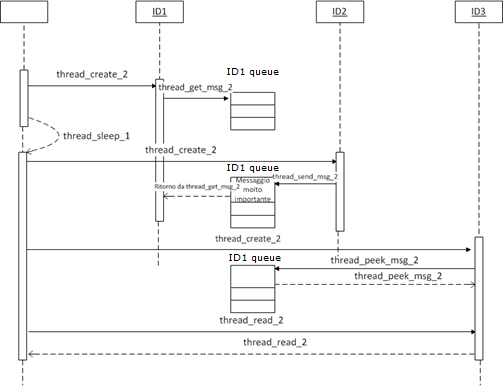
\includegraphics[width=12cm]{images/thread-example}
\caption{Execution flows in the third example.}
\label{fig:thread-example}
\end{figure}

\begin{verbatim}
start(X):- thread_create(ID1, thread1(ID1)),
           thread_sleep(200),
           thread_create(ID2, thread2(ID1)),
           thread_create(ID3, thread3(ID1,X)),
           thread_read(ID3, _),
           write('Father: done').

thread1(ID):- tell('threadLog.txt'),
              write('ID1: waiting for message'),
              thread_get_msg(ID, m(X)),
              write('ID1: message retrieved').

thread2(ID):- thread_send_msg( ID, m('critical message')),
              write('ID2: message sent').		

thread3(ID,X):- thread_peek_msg( ID, m(X)),
                write('ID3: trying to get message').
\end{verbatim}

More in detail, the father creates three threads identified by \texttt{ID1}, \texttt{ID2}, and \texttt{ID3}, which execute the goals \texttt{thread1/1}, \texttt{thread2/1}, and \texttt{thread3/2}, respectively: \texttt{ID1} is the message receiver/logger, \texttt{ID2} is the message sender, \texttt{ID3} is the task charged to monitor its brother's queue. To prevent races, the father waits for 200 ms after creating the first (message receiver) thread \texttt{ID1}, so that it is surely up and running when the message sender \texttt{ID2} and its brother \texttt{ID3} actually start.
Then, the father suspends its execution, waiting for \texttt{ID3} to terminate.

However, since \texttt{ID1} removes the message from its queue when reading (via \texttt{thread\_get\_msg/2}), \texttt{ID3} never finds anything when checking its brother's queue (via the non-blocking \texttt{thread\_peek\_msg/2} primitive): thus, its goal \texttt{thread3/2} always fails, causing the father's \texttt{thread\_read} to fail, too. As a result, the father's final write is never performed, either:

\begin{verbatim}
?- start(X).
no
\end{verbatim}
%
and the log file finally contains just

\begin{verbatim}
ID1: waiting for message
ID2: message sent
ID1: message retrieved
\end{verbatim}


%-------------------------------
\subsubsection{Synchronizing thread interactions}
%-------------------------------

In this producer/consumer example, the consumer's goal is to retrieve only the \textit{last} solution of the query \texttt{has\_child(bob,X)}, while the producer computes all the solutions to this query; the father coordinates the two tasks, by first creating the producer and the consumer, and then triggering the producer to generate all the possible solutions in sequence.

Without an explicit synchronisation mechanism, races would occur, causing the reader to read not \textit{the last} solution, but just ``one of'' the possible solutions, depending which thread is faster.

By suitably sequentialising the access to the producer's queue, the \texttt{mutex} semaphore guarantees that all solutions are produced \textit{before} the consumer can start reading, so that the last solution is actually read. (The execution flow diagram and the complete code are reported in Figure \ref{fig:thread-exampleMutex} on page \pageref{fig:thread-exampleMutex}.)

\begin{figure}
\centering
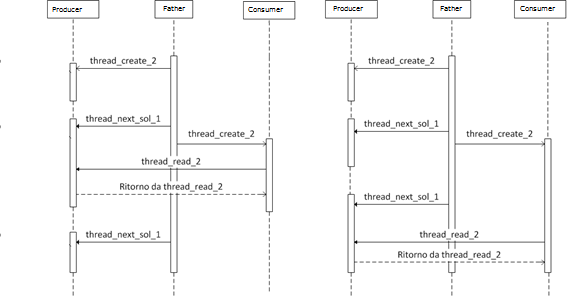
\includegraphics[width=13cm]{images/thread-exampleMutex}
\caption{Execution flows in the mutex example.}
%\label{fig:thread-exampleMutex}
%\end{figure}

\begin{Verbatim}[frame=single, samepage=true]
start:- thread_create(ID1, has_child(bob,X)),
        mutex_lock('mutex'),
        thread_create(ID2, read_child(ID1,X)),
        loop(1,5,1, ID1),
        mutex_unlock('mutex').

read_child(ID, X) :- mutex_lock('mutex'),
                     thread_read(ID, X),
                     mutex_unlock('mutex').

has_child(bob, alex).
has_child(bob, anna).
has_child(bob, mary).

loop(I, To, Inc, ThreadId) :- Inc >= 0, I > To, !.
loop(I, To, Inc, ThreadId) :- Inc < 0,  I < To, !.
loop(I, To, Inc, ThreadId) :-
  (thread_has_next(ThreadId) -> thread_next_sol(ThreadId),
                                Next is I+Inc,
                                loop(Next, To, Inc, ThreadId)
                              ; !).
\end{Verbatim}

\label{fig:thread-exampleMutex}
\end{figure}

The first child, \texttt{ID1}, is the solution finder \& producer: its task is to generate the solutions of the given goal \texttt{has\_child(bob,X)}. When started, it looks for the first solution: once found, it suspends waiting for possible future requests for alternative solutions. These will be actually asked shortly, since the father triggers \texttt{ID1} to find all the alternative solutions (via the \texttt{loop/4} predicate, which embeds a call to \texttt{thread\_next\_sol}) just after generating its second child, the solution reader thread \texttt{ID2}.
In fact, \texttt{ID2}'s task is to retrieve the computed solution from \texttt{ID1}'s private queue: but due to the \texttt{thread\_read} semantics, it actually reads \texttt{ID1}'s result only when \texttt{ID1} has terminated. This is why explicit synchronisation is needed: otherwise, the reader would read ``one of'' the solutions, non-deterministically, depending on which thread is faster (this can be easily checked by commenting out the \texttt{mutex\_lock}/\texttt{mutex\_unlock} statements).

With the explicit \texttt{mutex} semaphore, interactions are sequentialised: as long as the father holds the lock, the reader cannot retrieve any solution. Since the lock is released only after all the solutions have been explored, the reader will actually get only the last computed solution, \texttt{X / mary}.

%-------------------------------
\subsubsection{Flattening and manipulating lists}
%-------------------------------

Table \ref{tab:thread-exampleFlatList} on page \pageref{tab:thread-exampleFlatList} shows a sequential Prolog program that manipulates a list of (sub)lists. More precisely, it first flattens the list of lists into a single flat list, then sorts the obtained list and counts the occurrence of a given term in that list.

\begin{table}\small
\begin{Verbatim}[frame=single, samepage=true]
start(L, 0, T) :- !.
start([H|Tail], N, T) :-
    plain(H,L_plain),
    bubble(L_plain,L_ord),
    occurr_count(T,H,Count),
    C is N-1, start(Tail,C, T).

plain(L1,L2) :- plain(L1,[],L2).

plain([],ACC,ACC).
plain([H|REST],ACC,L2) :-
    H = [_|_],
    plain(H,ACC,ACC1),
    plain(REST,ACC1,L2).
plain([H|REST],ACC,L2) :-
    append(ACC,[H],ACC1),
    plain(REST,ACC1,L2).
plain(X,ACC,L2) :-
    append(ACC,[X],L2).

bubble(L1,L2) :- bubble(L1,0,L2).

bubble(L1,0,L2) :-
    sweep(L1,0,L2).
bubble(L1,0,L2) :-
    sweep(L1,1,LTMP),
    bubble(LTMP,0,L2).

sweep([X|[]],0,[X|[]]).
sweep([X,Y|REST1],CHANGED,[X|REST2]) :-
    X =< Y, sweep([Y|REST1],CHANGED,REST2).
sweep([X,Y|REST1],1,[Y|REST2]) :-
    X > Y, sweep([X|REST1],_,REST2).

occurr_count(T,L,N) :- occurr_count(T,L,0,N).

occurr_count(_,[],ACC,ACC).
occurr_count(T,[T|REST],ACC,N) :-
    ACC1 is ACC+1, occurr_count(T,REST,ACC1,N).
occurr_count(T,[_|REST],ACC,N) :- occurr_count(T,REST,ACC,N).
\end{Verbatim}
\caption{The sequential version of the list manipulation program.\\
         Query: \texttt{?- start([[[2,2],2,2,1],[4,[3],2],[9,8,9,2]], 3, 2).}}
\label{tab:thread-exampleFlatList}
\end{table}

To exploit concurrency, the program needs to be restructured, distributing the responsibilities among different threads.
As an example, we decided to delegate the list flattening and sorting to a child thread, maintaining the final occurrence counting on the main (father)'s thread: the result is shown in Table \ref{tab:thread-exampleFlatListConcurrent} on page \pageref{tab:thread-exampleFlatListConcurrent}, where the sequential and the concurrent versions are compared. The concurrent version showed a 16\% performance gain.

\begin{table}\small
\textit{Sequential version:}
\begin{Verbatim}[frame=single, samepage=true]
start(L, 0, T) :- !.
start([H|Tail], N, T) :-
    plain(H,L_plain),
    bubble(L_plain,L_ord),
    occurr_count(T,H,Count),
    C is N-1, start(Tail,C, T).
...
\end{Verbatim}

\textit{Concurrent version:}
\begin{Verbatim}[frame=single, samepage=true]
start(L, N, T) :-
    thread_create(ID, firstResp(L, N)),
    secondResp(L, N, T).

secondResp(L, 0, T):- !.
secondResp([H|Tail], N, T) :-
    occurr_count(T,H,Count),
    C is N-1, secondResp(Tail,C, T).

firstResp(L, 0) :- !.
firstResp([H|Tail], N) :-
    plain(H,L_plain),
    bubble(L_plain,L_ord),
    C is N-1, firstResp(Tail,C).
...
\end{Verbatim}
\caption{The sequential version (top) and the concurrent (bottom) version of the list manipulation program.\\
         Query: \texttt{?- start([[[2,2],2,2,1],[4,[3],2],[9,8,9,2]], 3, 2).}}
\label{tab:thread-exampleFlatListConcurrent}
\end{table}




%---------------------------------------------------------------------
\section{DCGLibrary}
\label{sec:dgc-library}
%---------------------------------------------------------------------

\noindent \emph{Library Dependencies}: BasicLibrary.

This library provides support for Definite Clause Grammars (DCGs) \cite{bra00}, an extension of context free grammars that have proven useful for describing natural and formal languages, and that may be conveniently expressed and executed in Prolog.
%
Note that this library is not loaded by default when a \tuprolog{} engine is created: it must be explicitly loaded by the user, or via a \texttt{load\_library} directive inside any theory using DCGs.

A DCG rule has the general form \verb|Head --> Body|: to distinguish terminal from nonterminal symbols, a phrase (that is, a sequence of terminal symbols) must be written as a Prolog list, with the empty sequence written as the empty list \verb|[]|.
%
The body can contain also executable blocks in parentheses, which are interpreted as normal Prolog rules.

Here is a simple example (see also Figure \ref{fig:dcg-example} on page \pageref{fig:dcg-example}):
%
\begin{verbatim}
    sentence --> noun_phrase, verb_phrase.
    verb_phrase --> verb, noun_phrase.
    noun_phrase --> [charles].
    noun_phrase --> [linda].
    verb --> [loves].
\end{verbatim}
%
To verify whether a phrase is correct according to the given grammar, the \texttt{phrase/2} or \texttt{phrase/3} predicates are used---the latter form providing an extra argument for the `remainder' of the input string not recognised as being part of the phrase.
%
Some examples follow:\\

\verb|?- phrase(sentence, [charles, loves, linda])|

\texttt{\textit{yes}}\\

\verb|?- phrase(sentence, [Who, loves, linda])|

\texttt{\textit{Who/charles}}

\texttt{\textit{Who/linda}}\\

\verb|?- phrase(sentence, [charles, loves, linda, but, hates, laura], R)|

\texttt{\textit{R/[but, hates, laura]}}\\

\begin{figure}
\centering
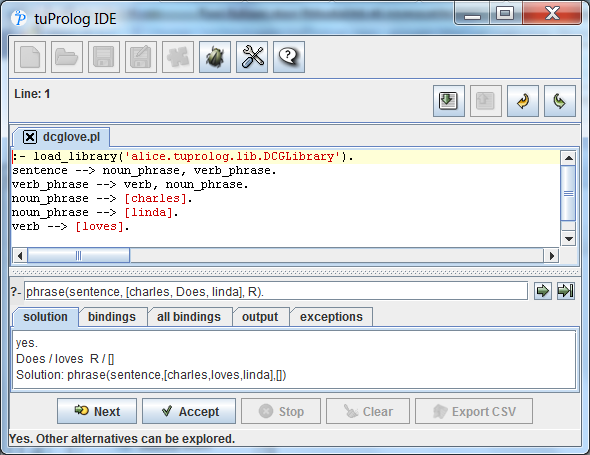
\includegraphics[width=7cm]{images/dcg-example}
\caption{The DCG Library example in the \tuprolog{} GUI (note the explicit library loading directive).}
\label{fig:dcg-example}
\end{figure}

%---------------------------------------------------------------------
\subsection{Predicates}
%---------------------------------------------------------------------

\noindent The classic built-in predicates provided for parsing DCG
sentences are:

\begin{itemize}
%
\item \bti{phrase/2}\\
    \noindent\bt{phrase(Category, List)} is true iff the list \bt{List} can be parsed as a phrase (i.e. sequence of terminals) of type \bt{Category}.
    \bt{Category} can be any term which would be accepted as a nonterminal of the grammar (or in general, it can be any grammar rule body), and must be instantiated to a non-variable term at the time of the call.
    This predicate is the usual way to commence execution of grammar rules.
    If \bt{List} is bound to a list of terminals by the time of the call, the goal corresponds to parsing \bt{List} as a phrase of type \bt{Category}; otherwise if \bt{List} is unbound, then the grammar is being used for generation.

    \template{phrase(+term, ?list)}

    \exception{error(instantiation\_error, instantiation\_error(\\
    Goal, ArgNo))} if \texttt{Category} is a variable. \texttt{Goal} is the goal where the problem occurred, \texttt{ArgNo} indicates the argument that caused the problem (obviously, \texttt{1}).

\item \bti{phrase/3}\\
    \noindent\bt{phrase(Category, List, Rest)} is true iff the segment between the start of list \bt{List} and the start of list \bt{Rest} can be parsed as a phrase (i.e. sequence of terminals) of type \bt{Category}.
    In other words, if the search for phrase Phrase is started at the beginning of list \bt{List}, then \bt{Rest} is what remains unparsed after \bt{Category} has been found.
    Again, \bt{Category} can be any term which would be accepted as a nonterminal of the grammar (or in general, any grammar rule body), and must be instantiated to a non variable term at the time of the call.

    \template{phrase(+term, ?list, ?rest)}

    \exception{error(instantiation\_error, instantiation\_error(\\
    Goal, ArgNo))} if \texttt{Category} is a variable. \texttt{Goal} is the goal where the problem occurred, \texttt{ArgNo} indicates the argument that caused the problem (obviously, \texttt{1}).

\end{itemize}

%---------------------------------------------------------------------
\subsection{Operators}
%---------------------------------------------------------------------

The full list of DCGLibrary operators, with their priority and associativity, is reported in Table \ref{tab:dcglibrary-operators}.

\begin{table}[h]
    \begin{center}{\small\tt
    \begin{tabular}{p{2cm}|p{3cm}|p{3cm}}\hline\hline
    Operator & Associativity & Priority \\ \hline
    --> & xfx & 1200\\
    \hline\hline
    \end{tabular}
    }\end{center}
    \caption{DCGLibrary operators.}\label{tab:dcglibrary-operators}
\end{table}


%---------------------------------------------------------------------
\section{ISOIOLibrary}
\label{sec:isoio-library}
%---------------------------------------------------------------------

The ISO specification requires a lot of I/O predicates---many more than \tuprolog{} IOLibrary supports.
%
Table \ref{fig:isoiolibrary-table} summarises the differences between \tuprolog{} IOLibrary and the ISO specifications.
%
\begin{figure}
  \centering
  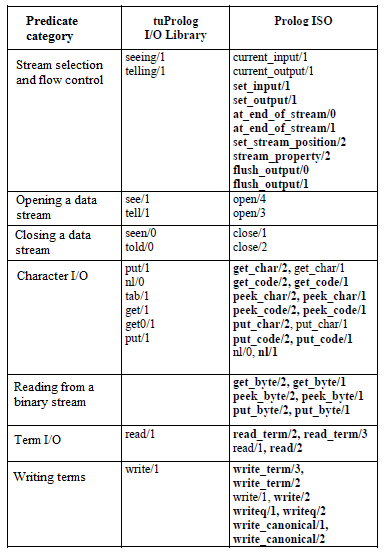
\includegraphics[width=10cm]{images/isoiolibrary-table}
  \caption{Comparison between the I/O predicates provided by IOLibrary and the ISO standard specification. Bold style indicates missing predicates, plain style indicates existing functionalities to be refactored, improved, or be provided with a different signature to be ISO-compliant.}\label{fig:isoiolibrary-table}
\end{figure}
%
The main reason for such a large number of differences is that the ISO Prolog standard defines very general concepts for I/O handling, aimed at supporting a wide variety of I/O modes and devices. More precisely:
\begin{itemize}
  \item \textbf{Sources} represent the resources from which data are read;
  \item \textbf{Sinks} represent the resources to which data are written.
\end{itemize}
%
Sources and sinks can be file, standard input/output stream, or any other resource supported by the underlying system: the only assumption is that each resource is associated to a sequence of bytes or characters.

\textit{Stream terms} provide a logical view of sources and sinks, and are used to identify a stream in I/O predicates. A stream term is a term respecting the following constraints:
\begin{itemize}
  \item it is a ground term;
  \item it is not an atom (this requirement means to distinguish stream terms from stream aliases--see below for details);
  \item it is not used to identify other streams at the same time.
\end{itemize}
%
The ISO standard does not specify whether the stream terms must result from an explicit source/sink opening by the \texttt{open/4} predicate, nor whether different sources/sinks must be represented by different stream terms at subsequent times: these issues are left to the specific implementation.

Moreover, each stream can be associated to a \textit{stream alias}---an atom used to refer to the stream. The association between a stream and its alias is created when the stream is opened, and automatically canceled when the stream is closed.
The same stream can be associated to multiple aliases simultaneously.
%
Two pre-defined streams exist that are always automatically open: the standard input (alias \texttt{user\_input}) and the standard output
(alias \texttt{user\_output}). Such streams must never be closed.

The ISO standard also introduces the concepts of \textit{current input stream} and \textit{current output stream}: initially, they default to the standard input and standard output above, but can be reassigned at any time via the \texttt{set\_input/1} e and \texttt{set\_output/1} predicates.
However, when such an input/output stream is closed, the current input/output stream must be re-set to its default value (i.e., the standard input/output, respectively).

One further concept is the \textit{stream position}, which defines the point where the next input/output will take place; syntactically, it is an implementation-dependent ground term.
The stream position is always supported, even by predicates whose operations do not change the position itself; to change the current position, the \texttt{set\_stream\_position/2} predicate is used.
When an output stream is repositioned, any output possibly present in the sink is overwritten; when an input stream is repositioned, instead, the content already available into the stream remains unaltered.

A stream that can be repositioned (that is, whose \texttt{reposition} property is true) must support also the \textit{end position} concept: the position of an input stream that has been completely read is represented by the \texttt{end-of-stream} atom, while any attempt to read beyond the end of stream causes the stream position to become \texttt{past-end-of-stream}.

On the other hand, output streams can be \textit{flushed} when necessary via the \texttt{flush\_output/1} predicate; a stream is automatically flushed before closing.


%---------------------------------------------------------------------
\subsection{Predicates}
%---------------------------------------------------------------------

\noindent ISOIOLibrary defines the following predicates:

\begin{itemize}

\item \bti{current\_input/1}\\
    \noindent\bt{current\_input} unifies the current input stream with the given argument.

    \template{current\_input(@Stream\_or\_alias)}

\item \bti{current\_output/1}\\
    \noindent\bt{current\_output} unifies the current output stream with the given argument.

    \template{current\_output(@Stream\_or\_alias)}


\item \bti{set\_input/1}\\
    \noindent\bt{set\_input} associates the current input to the provided argument, which can be either a stream\_term or an alias.

    \template{set\_input(@Stream\_or\_alias)}

    \exception{error(instantiation\_error, instantiation\_error)} if \textit{\texttt{Stream\_or\_alias}} is a variable.

    \exception{error(domain\_error, domain\_error(\texttt{stream\_or\_alias},\\
    \texttt{\textit{Stream\_or\_alias}}))} if \textit{\texttt{Stream\_or\_alias}} is neither a stream term nor a valid stream alias.

    \exception{error(existence\_error, existence\_error(\texttt{stream},\\
    \texttt{\textit{Stream\_or\_alias}}))} if \textit{\texttt{Stream\_or\_alias}} is not associated to an open stream.

    \exception{error(permission\_error, permission\_error(\texttt{input},\\
    \texttt{stream}, \texttt{\textit{Stream\_or\_alias}}))} if \textit{\texttt{Stream\_or\_alias}} is associated to an output stream.


\item \bti{set\_output/1}\\
    \noindent\bt{set\_output} associates the current output to the provided argument, which can be either a stream\_term or an alias.

    \template{set\_output(@Stream\_or\_alias)}

    \exception{error(instantiation\_error, instantiation\_error)} if \textit{\texttt{Stream\_or\_alias}} is a variable.

    \exception{error(domain\_error, domain\_error(\texttt{stream\_or\_alias},\\
    \texttt{\textit{Stream\_or\_alias}}))} if \textit{\texttt{Stream\_or\_alias}} is neither a stream term nor a valid stream alias.

    \exception{error(existence\_error, existence\_error(\texttt{stream},\\
    \texttt{\textit{Stream\_or\_alias}}))} if \textit{\texttt{Stream\_or\_alias}} is not associated to an open stream.

    \exception{error(permission\_error, permission\_error(\texttt{output},\\
    \texttt{stream}, \texttt{\textit{Stream\_or\_alias}}))} if \textit{\texttt{Stream\_or\_alias}} is associated to an input stream.

\item \bti{flush\_output/0} - \bti{flush\_output/1}\\
    \noindent\bt{flush\_output} flushes the output onto the stream associated to the provided argument, which can be either a stream\_term or an alias; if no argument is provided, the default output stream is flushed.

    \template{flush\_output(@Stream\_or\_alias)}\\
    \template{flush\_output}

    \exception{error(instantiation\_error, instantiation\_error)} if \textit{\texttt{Stream\_or\_alias}} is a variable.

    \exception{error(domain\_error, domain\_error(\texttt{stream\_or\_alias},\\
    \texttt{\textit{Stream\_or\_alias}}))} if \textit{\texttt{Stream\_or\_alias}} is not a valid stream term or alias.

    \exception{error(existence\_error, existence\_error(\texttt{stream},\\
    \texttt{\textit{Stream\_or\_alias}}))} if \textit{\texttt{Stream\_or\_alias}} is not associated to an open stream.

    \exception{error(permission\_error, permission\_error(\texttt{output},\\
    \texttt{stream}, \texttt{\textit{Stream\_or\_alias}}))} if \textit{\texttt{Stream\_or\_alias}} is associated to an input stream.


\item \bti{stream\_property/2}\\
    \noindent\bt{stream\_property} verifies whether the given stream has the given property, unifying \textit{\texttt{Property}} with the corresponding value.

    \template{stream\_property(?Stream, ?Property)}

    \exception{error(instantiation\_error, instantiation\_error)} if \textit{\texttt{Stream}} is a variable.

    \exception{error(domain\_error, domain\_error(\texttt{stream},\\
    \texttt{\textit{Stream}}))} if \textit{\texttt{Stream}} is not a stream term.

    \exception{error(domain\_error, domain\_error(\texttt{stream\_property},\\
    \texttt{\textit{Property}}))} if \textit{\texttt{Property}} is neither a variable nor a stream property.

    \exception{error(existence\_error, existence\_error(\texttt{stream},\\
    \texttt{\textit{Stream}}))} if \textit{\texttt{Stream}} is not associated to an open stream.


\item \bti{at\_end\_of\_stream/0} - \bti{at\_end\_of\_stream/1}\\
    \noindent\bt{at\_end\_of\_stream} succeeds if the \texttt{end\_of\_stream} property has either the \texttt{end\_of\_stream} or the \texttt{past\_end\_of\_stream} value. The zero-argument version checks the current input stream.

    \template{at\_end\_of\_stream(@Stream\_or\_alias)}\\
    \template{at\_end\_of\_stream}

    \exception{error(instantiation\_error, instantiation\_error)} if \textit{\texttt{Stream\_or\_alias}} is a variable.

    \exception{error(domain\_error, domain\_error(\texttt{stream},\\
    \texttt{\textit{Stream\_or\_alias}}))} if \textit{\texttt{Stream\_or\_alias}} is not a valid stream term or alias.

    \exception{error(existence\_error, existence\_error(\texttt{stream},\\
    \texttt{\textit{Stream\_or\_alias}}))} if \textit{\texttt{Stream\_or\_alias}} is not associated to an open stream.


\item \bti{set\_stream\_position/2}\\
    \noindent\bt{set\_stream\_position} is true if the stream position can be successfully set to the new \texttt{\textit{Position}} argument.

    \template{set\_stream\_position(@Stream\_or\_alias, @Position)}

    \exception{error(instantiation\_error, instantiation\_error)} if either \textit{\texttt{Stream\_or\_alias}} or \textit{\texttt{Position}} is a variable.

    \exception{error(domain\_error, domain\_error(\texttt{stream},\\
    \texttt{\textit{Stream\_or\_alias}}))} if \textit{\texttt{Stream\_or\_alias}} is not a valid stream term or alias.

    \exception{error(existence\_error, existence\_error(\texttt{stream},\\
    \texttt{\textit{Stream\_or\_alias}}))} if \textit{\texttt{Position}} is neither a valid stream position, nor a variable.

    \exception{error(permission\_error, permission\_error(\texttt{reposition},\\
    \texttt{stream}, \texttt{\textit{Stream\_or\_alias}}))} if the \texttt{reposition} property of this stream is false.


\item \bti{open/3} - \bti{open/4}\\
    \noindent\bt{open} succeeds if the stream can be opened according to the \texttt{mode} and \texttt{options} desired.

    \template{open(@Source\_Sink, @Mode, -Stream)}\\
    \template{open(@Source\_Sink, @Mode, -Stream, @Options)}

    \exception{error(instantiation\_error, instantiation\_error)} if either \textit{\texttt{Source\_sink}} or \textit{\texttt{Mode}} is a variable, or if \texttt{\textit{Options}} is a partial list or such a list contains a variable.

    \exception{error(type\_error, type\_error(atom, Mode))} if \textit{\texttt{Mode}} is a neither an atom nor a variable.

    \exception{error(type\_error, type\_error(list, Options))} if\\ \texttt{\textit{Options}} is neither a list nor a partial list.

    \exception{error(type\_error, type\_error(variable, Stream))} if \texttt{\textit{Stream}} is not a variable.

    \exception{error(domain\_error, domain\_error(\texttt{stream\_sink},\\
    \texttt{\textit{Source\_sink}}))} if \textit{\texttt{Source\_sink}} is not a valid stream source or sink.

    \exception{error(domain\_error, domain\_error(\texttt{io\_mode},\\
    \texttt{\textit{Mode}}))} if \textit{\texttt{Mode}} is an atom other than the prescribed \texttt{input} or \texttt{output}.

    \exception{error(domain\_error, domain\_error(\texttt{stream\_option},\\
    \texttt{\textit{Element}}))} if an \textit{\texttt{Element}} of the options list is neither a variable nor a valid stream option.

    \exception{error(existence\_error, existence\_error(\texttt{stream},\\
    \texttt{\textit{Source\_sink}}))} if the source /sink stream \textit{\texttt{Source\_sink}} does not exist.

    \exception{error(permission\_error, permission\_error(\texttt{open},\\
    \texttt{source\_sink}, \texttt{\textit{Source\_sink}}))} if the specified source/sink stream cannot be opened.

    \exception{error(permission\_error, permission\_error(\texttt{open},\\
    \texttt{source\_sink}, \texttt{alias(\textit{A})}))} if \texttt{alias(\textit{A})} is in the options list, and \texttt{\textit{A}} is already bound to another open stream.

    \exception{error(permission\_error, permission\_error(\texttt{open},\\
    \texttt{source\_sink}, \texttt{reposition(true)}))} if \texttt{reposition(true)} is in the options list, but the stream cannot be repositioned.


\item \bti{close/1} - \bti{close/2}\\
    \noindent\bt{close} closes the given stream, eliminating any associated alias(es).
    If the \texttt{force(true)} option is specified, the stream is immediately closed, ignoring any data not yet transferred (in the case of output streams); in any other case, the stream is flushed before closing. If the stream to be closed is the current stream, the latter will be associated to the standard input or output, as appropriate.

    \template{close(@Stream\_or\_alias)}\\
    \template{close(@Stream\_or\_alias, @Options)}

    \exception{error(instantiation\_error, instantiation\_error)} if either \textit{\texttt{Stream\_or\_alias}} is a variable, or \texttt{\textit{Options}} is a partial list or such a list contains a variable.

    \exception{error(type\_error, type\_error(list, Options))} if\\ \texttt{\textit{Options}} is neither a list nor a partial list.

    \exception{error(domain\_error, domain\_error(\texttt{stream\_or\_alias},\\
    \texttt{\textit{Stream\_or\_alias}}))} if \textit{\texttt{Stream\_or\_alias}} is not a valid stream term or alias.

    \exception{error(domain\_error, domain\_error(\texttt{close\_option},\\
    \texttt{\textit{Element}}))} if an \textit{\texttt{Element}} of the options list is neither a variable nor a valid close option.

    \exception{error(existence\_error, existence\_error(\texttt{stream},\\
    \texttt{\textit{Stream\_or\_alias}}))} if the stream \textit{\texttt{Stream\_or\_alias}} is not associated to an open stream.

    \exception{error(permission\_error, permission\_error(\texttt{open},\\
    \texttt{source\_sink}, \texttt{\textit{Source\_sink}}))} if the specified source/sink stream cannot be opened.

    \exception{error(permission\_error, permission\_error(\texttt{open},\\
    \texttt{source\_sink}, \texttt{alias(\textit{A})}))} if \texttt{alias(\textit{A})} is in the options list, and \texttt{\textit{A}} is already bound to another open stream.

    \exception{error(permission\_error, permission\_error(\texttt{open},\\
    \texttt{source\_sink}, \texttt{reposition(true)}))} if \texttt{reposition(true)} is in the options list, but the stream cannot be repositioned.


\item \bti{get\_char/2} - \bti{get\_char/1} - \bti{get\_code/2} - \bti{get\_code/1}\\
    \noindent\bt{get\_char} and \bt{get\_code} read the next char from the given stream, and unify it with the second argument---a character or an integer representing the character code, respectively; the single-argument version of these predicates read from the current input stream. Special cases are treated as follows:
    \begin{itemize}
      \item if the stream position is \texttt{past\_end\_of\_stream}, the action to be performed depends on the stream options specified when the stream was opened---namely, \texttt{eof\_action(\textit{Action})}(see above);
      \item if the stream position is \texttt{end\_of\_stream}, the EOF character is returned, and the stream position becomes \texttt{past\_end\_of\_stream}.
    \end{itemize}

    \template{get\_char(@Stream\_or\_alias, ?Character)}\\
    \template{get\_char(?Character)}\\
    \template{get\_code(@Stream\_or\_alias, ?Character\_code)}\\
    \template{get\_code(?Character\_code)}

    \exception{error(instantiation\_error, instantiation\_error)} if either \textit{\texttt{Stream\_or\_alias}} is a variable.

    \exception{error(type\_error, type\_error(in\_character, \textit{Character}))} if \texttt{\textit{Character}} is neither a variable nor a character.

    \exception{error(type\_error, type\_error(integer, \textit{Character\_code}))} if \texttt{\textit{Character\_code}} is neither a variable nor an integer.

    \exception{error(domain\_error, domain\_error(\texttt{stream\_or\_alias},\\
    \texttt{\textit{Stream\_or\_alias}}))} if \textit{\texttt{Stream\_or\_alias}} is not a valid stream term or alias.

    \exception{error(existence\_error, existence\_error(\texttt{stream},\\
    \texttt{\textit{Stream\_or\_alias}}))} if the stream \textit{\texttt{Stream\_or\_alias}} is not associated to an open stream.

    \exception{error(permission\_error, permission\_error(\texttt{input},\\
    \texttt{stream}, \texttt{\textit{Stream\_or\_alias}}))} if the stream in not an input stream.

    \exception{error(permission\_error, permission\_error(\texttt{input},\\
    \texttt{binary\_stream}, \texttt{\textit{Stream\_or\_alias}}))} if the stream in not a text stream.

    \exception{error(permission\_error, permission\_error(\texttt{input},\\
    \texttt{past\_end\_of\_stream}, \texttt{\textit{Stream\_or\_alias}}))} if the stream status is\\
    \texttt{end\_of\_stream(past)} and the option \texttt{eof\_action(true)} is active.

    \exception{error(representation\_error,  representation\_error(\texttt{\textit{\\
    Character}}))} if the entity read from the stream is not a character.

    \exception{error(representation\_error,  representation\_error(\texttt{\textit{\\
    Character\_code}}))} if the entity read from the input stream is an integer, but does not represent a character.


\item \bti{peek\_char/2} - \bti{peek\_char/1} - \bti{peek\_code/2} - \bti{peek\_code/1}\\
    \noindent\bt{peek\_char} and \bt{peek\_code} work identically to the \texttt{get\_char} and \texttt{get\_code} above, but leave the stream position unaltered after reading, so that a subsequent read operation returns the same character.

    \template{peek\_char(@Stream\_or\_alias, ?Character)}\\
    \template{peek\_char(?Character)}\\
    \template{peek\_code(@Stream\_or\_alias, ?Character\_code)}\\
    \template{peek\_code(?Character\_code)}

    \exception{}: the same as above.


\item \bti{put\_char/2} - \bti{put\_char/1} - \bti{put\_code/2} - \bti{put\_code/1}\\
    \noindent\bt{put\_char} and \bt{put\_code} are the writing counterparts of the \texttt{get\_char} and \texttt{get\_code} above; syntax and exceptions raised are basically identical, but the \texttt{Character} or \texttt{Character\_code} must be ground in this case---otherwise, an \texttt{instantiation\_error} occurs.

    \template{put\_char(@Stream\_or\_alias, +Character)}\\
    \template{put\_char(+Character)}\\
    \template{put\_code(@Stream\_or\_alias, +Character\_code)}\\
    \template{put\_code(+Character\_code)}

    \exception{}: the same as above, plus an \texttt{error(instantiation\_error, instantiation\_error)} if \texttt{Character} or \texttt{Character\_code} is a variable.

\item \bti{nl/0} - \bti{nl/1}\\
    \noindent\bt{nl} inserts a newline in the given stream.

    \template{nl(@Stream\_or\_alias)}\\
    \template{nl}

    \exception{error(instantiation\_error, instantiation\_error)} if either \textit{\texttt{Stream\_or\_alias}} is a variable.


\item \bti{read\_term/2} - \bti{read\_term/3} - \bti{read/1} - \bti{read/2}\\
    \noindent\bt{read\_term} succeeds if a term can be read from the given stream that can be unified with the \texttt{\textit{Term}} argument: \texttt{\textit{Options}} are considered only if the above unification succeeds. The \texttt{read} predicate works analogously, but no options can be specified. As usual, the no-stream versions (\bti{read\_term/2} and \bti{read/1}) operate on the current input stream.

    \template{read\_term(@Stream\_or\_alias, ?Term, +Options)}\\
    \template{read\_term(?Term, +Options)}\\
    \template{read(@Stream\_or\_alias, ?Term)}\\
    \template{read(?Term)}

    \exception{error(instantiation\_error, instantiation\_error)} if either \textit{\texttt{Stream\_or\_alias}} is a variable.

    \exception{error(instantiation\_error, instantiation\_error)} if \texttt{\textit{Options}} is either a partial list, or an element in the list is a variable.

    \exception{error(type\_error, type\_error(list, \textit{Options}))} if\\ \texttt{\textit{Options}} is neither a list nor a partial list.

    \exception{error(domain\_error, domain\_error(\texttt{stream\_or\_alias},\\
    \texttt{\textit{Stream\_or\_alias}}))} if \textit{\texttt{Stream\_or\_alias}} is not a valid stream term or alias.

    \exception{error(existence\_error, existence\_error(\texttt{stream},\\
    \texttt{\textit{Stream\_or\_alias}}))} if the stream \textit{\texttt{Stream\_or\_alias}} is not associated to an open stream.

    \exception{error(domain\_error, domain\_error(\texttt{read\_option},\\
    \texttt{\textit{Element}}))} if an element in the option list is neither a variable nor a valid read option.

    \exception{error(existence\_error, existence\_error(\texttt{stream},\\
    \texttt{\textit{Stream\_or\_alias}}))} if \textit{\texttt{Stream\_or\_alias}} is not associated to an open stream.

    \exception{error(permission\_error, permission\_error(\texttt{input},\\
    \texttt{stream}, \texttt{\textit{Stream\_or\_alias}}))} if the stream in not an input stream.

    \exception{error(permission\_error, permission\_error(\texttt{input},\\
    \texttt{binary\_stream}, \texttt{\textit{Stream\_or\_alias}}))} if the stream in not a text stream.

    \exception{error(permission\_error, permission\_error(\texttt{input},\\
    \texttt{past\_end\_of\_stream}, \texttt{\textit{Stream\_or\_alias}}))} if the stream status is\\
    \texttt{end\_of\_stream(past)} and the option \texttt{eof\_action(true)} is active.

    \exception{error(representation\_error,  representation\_error(\texttt{\textit{\\
    Flag}}))} if the entity read from the stream does not comply with the rules expressed by \texttt{\textit{Flag}}, which can be \texttt{max\_arity}, \texttt{max\_integer}, \texttt{min\_integer}.

    \exception{error(representation\_error,  representation\_error(\texttt{
    imp\_dep\_atom}))} if one or more characters in the input stream cannot form a valid token, or the character sequence cannot be transformed into a valid atom according to the current operator notation.

\item \bti{write\_term/2} - \bti{write\_term/3} - \bti{write/1} - \bti{write/2} - \bti{writeq/1} - \bti{writeq/2} - \bti{write\_canonical/1} - \bti{write\_canonical/2}\\
    These predicates are the writing counterparts of the \texttt{read\_term} and \texttt{read} predicates above: the given term is written on the given stream according to the specified write options, or following the default values\footnote{Namely: \texttt{quoted(false)}, \texttt{ignore\_ops(false)}, \texttt{numbervars(true)} for \texttt{write}, \texttt{quoted(true)}, \texttt{ignore\_ops(false)}, \texttt{numbervars(true)} for \texttt{writeq}, \texttt{quoted(true)}, \texttt{ignore\_ops(true)}, \texttt{numbervars(true)} for \texttt{write\_canonical}.} in the \texttt{write}, \texttt{writeq} and \texttt{write\_canonical} cases. Basically, the same considerations and exceptions above still apply.

    \template{write\_term(@Stream\_or\_alias, @Term, +Options)}\\
    \template{write\_term(@Term, +Options)}\\
    \template{write(@Stream\_or\_alias, @Term)}\\
    \template{write(@Term)}
    \template{writeq(@Stream\_or\_alias, @Term)}\\
    \template{writeq(@Term)}

    \exception{}: the same as above

%---------------------------------------------------------------------
%\subsubsection{Writing terms}
%---------------------------------------------------------------------

    When a term is written via \texttt{write\_term/3}, the following rules apply:

    \begin{itemize}
      \item if the term is a variable, a character is produced of the form \texttt{\_\textit{string}} where the string following the underscore are implementation-dependent. A variable occurring multiple times in the term is obviously converted into the same \texttt{\_\textit{string}} for each occurrence.
      \item if the term is an integer number, the corresponding string is produced; negative values starts with \texttt{-}.
      \item if the term is a real number, the corresponding string is produced; negative values starts with \texttt{-}. If the write option \texttt{quoted} is true, the produced string ensures that a subsequent \texttt{read\_term} can read it back correctly.
      \item if the term is an atom that could not be read back unless quoted, and the write option \texttt{quoted} is true, the produced string is quoted; otherwise it is not.
      \item if the term contains a main functor that \textit{is not} an operator, or the write option \texttt{ignore\_ops} is true, the term is written in the \textit{canonical form} (Table \ref{tab:isoiolibrary-write-terms}); otherwise it is not.
      \item if, instead, the term contains a main that \textit{is} an operator and the write option \texttt{ignore\_ops} is true, the term is written in the operator notation ((Table \ref{tab:isoiolibrary-write-terms}).
    \end{itemize}

    \begin{table}
      \footnotesize\centering
      \begin{tabular}{|p{6cm}|p{6cm}|}
        \hline
        \textit{Canonical form} & \textit{Operator notation}\\
        \hline
        For every term other than lists: & - The operator itself is returned either before
        (for prefix operators), or between (for infix operators) or after (for postfix operators) its arguments;\\
        - the main functor's atom; &  - a space is always inserted between the operator and its arguments;\\
        - the open parenthesis \texttt{'('}; & - for each argument, the same rules above are applied recursively; \\
        - each term argument, built applying the same rules recursively, in a comma-separated list; & - if one of the argument is also an operator, it is enclosed between parentheses. \\
        - the closed parenthesis \texttt{')'}; & \\
        \textbf{Example:} \texttt{2+3} becomes \texttt{+(2,3)} & \\
        \hline
        For lists (e.g. terms of the form \texttt{�.�(Head, Tail)}), the list notation is used if the write option \texttt{ignore\_ops} is false: & \\
        - an open square bracket \texttt{'['}; &  \\
        - the head argument, built applying the same rules recursively; & \\
        - the tail argument, built as follows; & \\
        \mbox{~~}- if the tail has the form \texttt{�.�(Head, Tail)}), a comma is produced and the above rule is triggered recursively; & \\
        \mbox{~~}- otherwise, if the tail is empty (e.g. \texttt{[]}), a close bracket is produced \texttt{']'} & \\
        \mbox{~~}- otherwise, a pipe symbol is produced \texttt{'|'} and these rules are re-applied recursively; at the end, a close bracket is produced \texttt{']'} & \\
        \hline
      \end{tabular}
      \caption{Term writing rules: canonical form and operator notation.}
      \label{tab:isoiolibrary-write-terms}
\end{table}


\item \bti{get\_byte/2} - \bti{get\_byte/1} - \bti{peek\_byte/2} - \bti{peek\_byte/1} - \bti{put\_byte/2} - \bti{put\_byte/1}\\
    \noindent\bt{get\_byte}, \bt{peek\_byte} and \bt{put\_byte} are the binary counterparts of the \texttt{get\_char}, \texttt{peek\_char} and \texttt{put\_char} above; syntax and exceptions raised are basically identical, with obvious changes (i.e., the wrong type of stream here is \texttt{text} instead of \texttt{binary}).

    \template{get\_byte(@Stream\_or\_alias, ?Byte)}\\
    \template{get\_byte(?Byte)}\\
    \template{peek\_byte(@Stream\_or\_alias, ?Byte)}\\
    \template{peek\_byte(?Byte)}\\
    \template{put\_byte(@Stream\_or\_alias, +Byte)}\\
    \template{put\_byte(+Byte)}

    \exception{}: see description above.

\end{itemize}





%---------------------------------------------------------------------
\subsection{Options}
%---------------------------------------------------------------------

The ISO standard defines options for stream creation, stream closure, and stream properties.

\noindent When a stream is opened via \texttt{open/4}:

\begin{itemize}
 \item \texttt{type(\textit{Type})} specifies the stream type---either a binary stream or a text stream (default);
 \item \texttt{reposition(\textit{Bool})} specifies whether the stream can be repositioned or not (see above);
 \item \texttt{alias(\textit{Alias})} defines \texttt{\textit{Alias}} as a stream alias for this stream;
 \item \texttt{eof\_action(\textit{Action})} specifies the value to be returned by a read predicate encountering the end-of-stream; possible values are \texttt{error}, to indicate that no further read is possible, or \texttt{eof\_code} \textit{(default)}, to indicate that the special \texttt{eof} value must be returned, or \texttt{reset}, meaning that the read position must be reset to the start of the stream. This is particulary useful on the console input.
\end{itemize}

\noindent Conversely, when a stream is closed via \texttt{close/1}-\texttt{/2}:

\begin{itemize}
 \item \texttt{force(\textit{Bool})} specifies whether the stream must be forcedly closed upon error: the default is \textit{false}. If the value is set to \textit{true}, the stream might remain in an inconsistent state, or data may be lost, when the forced closing occurs.
\end{itemize}

\noindent Stream properties are expressed via the \texttt{stream\_property(\textit{Stream}, \textit{Property})} predicate, where \texttt{\textit{Property}} is one of the following:

\begin{itemize}
 \item \texttt{file\_name(\textit{File})} if the stream is connected to a file, returns a unique identifier of the file;

  \item \texttt{mode(\textit{Mode})} is to be specified when the stream is opened: \texttt{\textit{Mode}} can be \texttt{read}, \texttt{write} or \texttt{append};

  \item \texttt{input} if the stream is connected to a source;

  \item \texttt{output} if the stream is connected to a sink;

  \item \texttt{alias(\textit{Alias})} returns the stream alias, if the stream has one;

  \item \texttt{position(\textit{Pos})} returns the current stream position, if the stream can be repositioned;

  \item \texttt{end\_of\_stream(\textit{End})} returns either \texttt{not}, if the stream is not at the end, or \texttt{at}, if the stream is precisely at the end, or \texttt{past} if the stream is past the end of the stream;

  \item \texttt{eof\_action(\textit{Action})} returns the \texttt{\textit{Action}} specified when the stream was opened, if there was one, or an implementation-dependent action associated to the stream, otherwise;

  \item \texttt{reposition(\textit{Bool})} returns whether the stream can be repositioned (\texttt{true} or \texttt{false});

  \item \texttt{type(\textit{Type})} returns whether the stream is a \texttt{binary} stream or a \texttt{text} stream.
\end{itemize}

\noindent The standard input and output streams are configured as in Table \ref{tab:isoiolibrary-user-streams}.

\begin{table}
  \centering
  \begin{tabular}{|p{5cm}|p{5cm}|}
    \hline
    \textbf{\texttt{user\_input}} & \textbf{\texttt{user\_output}}\\
    \hline
    \texttt{mode(read)} & \texttt{mode(append)} \\
    \texttt{input} & \texttt{output} \\
    \texttt{alias(user\_input)} & \texttt{alias(user\_output)}\\
    \texttt{eof\_action(reset)} & \texttt{eof\_action(reset)}\\
    \texttt{reposition(false)} & \texttt{reposition(false)}\\
    \texttt{type(text)} & \texttt{type(text)}\\
    \hline
  \end{tabular}
  \caption{The default configuration of the standard I/O streams.}
  \label{tab:isoiolibrary-user-streams}
\end{table}


\noindent Read properties can be specified in read predicates like \texttt{read\_term}, and can have the following forms:

\begin{itemize}
 \item \texttt{variables(\textit{Vars})}: when a term is read, \texttt{\textit{Vars}} is the list of variables found in the term; anonymous variables are included;

 \item \texttt{variable\_names(\textit{VNList})}: when a term is read, \texttt{\textit{VNList}} is unified with a list of \texttt{A=V} pairs, where \texttt{A} is an atom denoting a variable name in term read, and \texttt{V} is the corresponding variable in the term template; anonymous variables are not included in the list;

 \item \texttt{singletons(\textit{VNList})}: when a term is read, \texttt{\textit{VNList}} is unified with a list of \texttt{A=V} pairs, where \texttt{A} is an atom denoting a variable name in term read, and \texttt{V} is the corresponding variable in the term template; anonymous variables are not included in the list.
\end{itemize}

\noindent For instance, if a query like:

\texttt{?:- read\_term(st, T, [variables(VL),\\
\mbox{~~~~~~~~~~~~~~~~~~~~~~~~~}variable\_names(VN), singletons(VS)].}

\noindent reads a term such as \texttt{foo(A+Roger, A+\_)}, the result is:

\noindent
\texttt{T  / foo(Xl+X2, X1+X3)}\\
\texttt{VL / [Xl, X2, X3]}\\
\texttt{VN / ['A' = Xl, 'Roger' = X2]}\\
\texttt{VS / ['Roger' = X2]}

\noindent Basically, the term read is scanned for variables, which are named according to some implementation-dependent template (e.g. \texttt{X1}, \texttt{X2}, \texttt{X3}); these names are used in the lists above, either to list all the variables (including the anonymous ones---see \texttt{X3} in \texttt{VL}), or to list the correspondence between the actual variable names and such placeholders (\texttt{VN} and \texttt{VS}, the latter including singleton variables only).

Analogously, write properties can be specified in write predicates like \texttt{write\_term}, and can have the following forms:

\begin{itemize}
 \item \texttt{quoted(\textit{Bool})}: specifies whether each atom of functor is quoted (usually because it comes from a previous \texttt{read\_term});

 \item \texttt{ignore\_ops(\textit{Bool})}: if true, each compound term is returned in a function notation. Any other option is ignored.

 \item \texttt{numbervars(\textit{Bool})}: if true, the terms of the form \texttt{'\$VAR'(N)} are replaced by a system-generated variable name that uses the \textit{N}th capital letter\footnote{\texttt{A} is considered the 0th letter.} followed by a the \texttt{N}/26 integer.
     For instance, \texttt{'\$VAR'(51)} produces \texttt{Z1}, since the 51th letter of the alphabet (mod 26) is \texttt{Z}, and 51/26=1.
\end{itemize}


%---------------------------------------------------------------------
\section{SocketLibrary}
\label{sec:socket-library}
%---------------------------------------------------------------------

\noindent \emph{Library Dependencies}: BasicLibrary.

This library provides support for TCP and UDP sockets. To this end, the library provides functionalities for
\begin{itemize}
  \item handling server sockets---namely, creating and closing a server socket, and accepting incoming connections;
  \item handling client sockets---namely, opening a socket establishing a connection to a given address;
  \item handling client/server communication, both in synchronous and asynchronous mode.
\end{itemize}

As an example, let us first consider the following TCP server-side code:\\

\begin{verbatim}
server(X,Y,Z):- tcp_socket_server_open('127.0.0.1:4444', Sock,[]),
                tcp_socket_server_accept(Sock,ClientAddr,Slave),
                read_from_socket(Slave,X,[]),
                write_to_socket(Slave,echo(X)),
                read_from_socket(Slave,Y,[]),
                write_to_socket(Slave,echo(Y)),
                read_from_socket(Slave,Z,[]),
                write_to_socket(Slave,echo(Z)),
                tcp_socket_server_close(Sock).
\end{verbatim}

\noindent to be coupled with the following TCP client-side code:\\

\begin{verbatim}
client(X,Y,Z):- tcp_socket_client_open('127.0.0.1:4444',Sock),
                write_to_socket(Sock,test1),
                read_from_socket(Sock,X,[]),
                write_to_socket(Sock,test2),
                read_from_socket(Sock,Y,[]),
                write_to_socket(Sock,test3),
                read_from_socket(Sock,Z,[]).
\end{verbatim}

\noindent In this scenario, the client opens a connection towards the server -- that is supposed to be already up and running, waiting connection requests on its server socket  -- and starts exchanging messages with the server.


In the UDP case, the same example would become:\\

\begin{verbatim}
server(X):- udp_socket_open('127.0.0.1:4445',Sock2),
            udp_receive(Sock2, X , '127.0.0.1:4444',[]),
            udp_socket_close(Sock2).
\end{verbatim}

\noindent to be coupled with the following UDP client:\\

\begin{verbatim}
client(X):- udp_socket_open('127.0.0.1:4444',Sock),
            udp_send(Sock, test1,'127.0.0.1:4444'),
            udp_socket_close(Sock).
\end{verbatim}


%---------------------------------------------------------------------
\subsection{Predicates}
%---------------------------------------------------------------------

\noindent The following socket handling predicates are provided:

\begin{itemize}
%
\item \bti{tcp\_socket\_server\_open/3}\\
    \noindent\bt{tcp\_socket\_server\_open(+Address, -Socket, +Options)} is true iff \bt{Address} represents a valid Internet address, and \bt{Socket} can be unified with a newly-created server socket; \bt{Options} is a possibly-empty list of options---currently, only the maximum number od connection request can be specified in the form of the \texttt{backlog(\textit{N})} term: if unspecified, the default value is \texttt{backlog(0)}, meaning the queue is unlimited.

    \template{tcp\_socket\_server\_open(+term, -term, +list)}

    \exception{error(instantiation\_error, instantiation\_error(\\
    Goal, ArgNo))} if \texttt{Socket} is not a variable, or the address length is not equal to 5 during the transformation of \texttt{Address} from the \texttt{IP:Port} form to the byte array and port number inner form.

\item \bti{tcp\_socket\_server\_accept/3}\\
    \noindent\bt{tcp\_socket\_server\_accept(+ServerSocket, -ClientAddress,\\
    -ClientSlaveSocket)} is true iff \bt{ServerSocket} represents a valid server socket address, and \bt{ClientAddress} can be unified with the client address in the \texttt{\textit{Address}:\textit{Port}} form, and \bt{ClientSlaveSocket} can be unified with the newly-created client socket.

    \template{tcp\_socket\_server\_accept(+term, -term, -term)}

    \exception{error(instantiation\_error, instantiation\_error(\\
    Goal, ArgNo))} if \texttt{ServerSocket} is a variable, or is not bound to server socket.

\item \bti{tcp\_socket\_server\_close/1}\\
    \noindent\bt{tcp\_socket\_server\_close(+ServerSocket)} is true iff \bt{ServerSocket} represents a valid server socket; as a side effect, the socket is closed.

    \template{tcp\_socket\_server\_close(+term)}

    \exception{error(instantiation\_error, instantiation\_error(\\
    Goal, ArgNo))} if \texttt{ServerSocket} is a variable, or is not bound to server socket.

\item \bti{tcp\_socket\_client\_open/2}\\
    \noindent\bt{tcp\_socket\_client\_open(+Address, -Socket)} is true iff \bt{Address} represents a valid Internet address in the \texttt{\textit{Address}:\textit{Port}} form, a server is waiting for incoming connection at that address, and \texttt{Socket} is unified with a newly-created socket.

    \template{tcp\_socket\_client\_open(+term, -term)}

    \exception{error(instantiation\_error, instantiation\_error(\\
    Goal, ArgNo))} if \texttt{Socket} is not a variable, or the address length is not equal to 5 during the transformation of \texttt{Address} from the \texttt{IP:Port} form to the byte array and port number inner form.

\item \bti{write\_to\_socket/2}\\
    \noindent\bt{write\_to\_socket(+Socket, +Msg)} is true iff \bt{Socket} represents a valid socket with an open associated output stream, and \texttt{Msg} is a valid term representing the message to be sent; as a side effect, the message is sent onto the stream.

    \template{write\_to\_socket(+term, +term)}

    \exception{error(instantiation\_error, instantiation\_error(\\
    Goal, ArgNo))} if \texttt{Socket} is a variable, or is not bound to client socket, or \texttt{Msg} is a variable.

\item \bti{read\_from\_socket/2}\\
    \noindent\bt{read\_from\_socket(+Socket, -Msg, +Options)} is true iff \bt{Socket} represents a valid socket with an open associated input stream, and \texttt{Options} is a valid option list---currently, only a timeout in milliseconds can be specified; as a side effect, a message is read from the stream and unified with \texttt{Msg}. If no message is available, the primitive suspends until one arrives (synchronous behaviour).

    \template{read\_from\_socket(+term, -term, +list)}

    \exception{error(instantiation\_error, instantiation\_error(\\
    Goal, ArgNo))} if \texttt{Socket} is a variable, or is not bound to client socket, or \texttt{Msg} is a variable.

\item \bti{aread\_from\_socket/2}\\
    \noindent\bt{aread\_from\_socket(+Socket, +Options)} is the asynchronous version of the above primitive; again, it is true iff \bt{Socket} represents a valid socket with an open associated input stream, and \texttt{Options} is a valid option list. As a side effect, a message is eventually read from the stream and asserted into the current prolog theory via \texttt{asserta}.
    Two options are available: the first makes it possible to set a timeout in milliseconds, as above; the other makes it possible to specify that the message is eventually asserted at the end of the current theory (i.e. via \texttt{assertz}) instead of at the top (i.e. via \texttt{asserta}, the default behaviour).

    \template{aread\_from\_socket(+term, +list)}

    \exception{error(instantiation\_error, instantiation\_error(\\
    Goal, ArgNo))} if \texttt{Socket} is a variable, or is not bound to client socket (only client sockets can asynchronously read from a server).

\item \bti{udp\_socket\_open/2}\\
    \noindent\bt{udp\_socket\_open(+Address, -DatagramSocket)} is true iff \bt{Address} represents a valid Internet address in the \texttt{\textit{Address}:\textit{Port}} form, a server is waiting for incoming connection at that address, and \texttt{DatagramSocket} is unified with a newly-created datagram socket.

    \template{udp\_socket\_open(+term, -term)}

    \exception{error(instantiation\_error, instantiation\_error(\\
    Goal, ArgNo))} if \texttt{Socket} is not a variable, or the address length is not equal to 5 during the transformation of \texttt{Address} from the \texttt{IP:Port} form to the byte array and port number inner form.

\item \bti{udp\_socket\_close/1}\\
    \noindent\bt{udp\_socket\_close(DatagramSocket)} is true iff \bt{DatagramSocket} represents a valid datagram socket; as a side effect, the socket is closed.

    \template{udp\_socket\_close(+term)}

    \exception{error(instantiation\_error, instantiation\_error(\\
    Goal, ArgNo))} if \texttt{DatagramSocket} is a variable, or is not bound to datagram socket.

\item \bti{udp\_send/3}\\
    \noindent\bt{udp\_send(-DatagramSocket, +Msg, +AddressTo)} is true iff \texttt{Msg} is a valid term representing the message to be sent, and \texttt{AddressTo} represents the destination address in the \texttt{\textit{Address}:\textit{Port}} form; as a side effect, \bt{DatagramSocket} is bound to the datagram socket associated to the output stream, and the message is sent onto the stream.

    \template{udp\_send(+term, +term, +term)}

    \exception{error(instantiation\_error, instantiation\_error(\\
    Goal, ArgNo))} if \texttt{DatagramSocket} is a not variable, or the address length is not equal to 5 during the transformation of \texttt{AddressTo} from the \texttt{IP:Port} form to the byte array and port number inner form.

\item \bti{udp\_receive/4}\\
    \noindent\bt{udp\_receive(-DatagramSocket, -Msg, +AddressTo, +Options)} is true iff \\
    \texttt{AddressTo} represents the destination address in the \texttt{\textit{Address}:\textit{Port}} form, and \texttt{Options} is a possibly-empty option list; currently, the available options are \texttt{max\_msg\_size(+\textit{Size})}, whose default value is 4096 bytes, and \texttt{timeout(+\textit{Time})}, which specifies a timeout: a value of 0 stands for infinite waiting.
    Upon reception of a message, as a side effect, the \texttt{Msg} term is unified with the incoming message, and
    \bt{DatagramSocket} is bound to a datagram socket associated to the input stream.

    \template{udp\_receive(+term, +term, +term, +list)}

    \exception{error(instantiation\_error, instantiation\_error(\\
    Goal, ArgNo))} if \texttt{DatagramSocket} is not a variable, or the address length is not equal to 5 during the transformation of \texttt{AddressTo} from the \texttt{IP:Port} form to the byte array and port number inner form.

\end{itemize}

%---------------------------------------------------------------------
\subsection{Operators}
%---------------------------------------------------------------------

No operators are defined in this library.

%The full list of SocketLibrary operators, with their priority and associativity, is reported in Table \ref{tab:socketlibrary-operators}.
%
%\begin{table}[h]
%    \begin{center}{\small\tt
%    \begin{tabular}{p{2cm}|p{3cm}|p{3cm}}\hline\hline
%    Operator & Associativity & Priority \\ \hline
%%    --> & xfx & 1200\\
%    \hline\hline
%    \end{tabular}
%    }\end{center}
%    \caption{SocketLibrary operators.}\label{tab:socketlibrary-operators}
%\end{table}

%---------------------------------------------------------------------
\subsection{Use from the Java side: term hierarchy extension}
%---------------------------------------------------------------------

In order to support the use of sockets from the Java side, SocketLibrary enhances the Term hierarchy by
introducing four further \texttt{Term} types that represent sockets: more precisely, \texttt{AbstractSocket} (a direct child of \texttt{Term}) represents the generic socket, whose concrete realisations are provided by its three children--- \texttt{Client\_Socket} and \texttt{Server\_Socket} in the TCP case, \texttt{Dataggram\_Socket} in the UDP case.

Consequently, \texttt{AbstractSocket} redefines some \texttt{Term} methods and defines some new abstract methods, implemented in the derived classes \texttt{Client\_Socket} and \texttt{Server\_Socket}:
\begin{itemize}
  \item \texttt{public abstract boolean isClientSocket();}
  \item \texttt{public abstract boolean isServerSocket();}
  \item \texttt{public abstract boolean isDatagramSocket();}
  \item \texttt{public abstract Object getSocket();}
  \item \texttt{public abstract InetAddress getAddress();}
\end{itemize}

\noindent In order to show the use of the SocketLibrary functions from Java, here are some small code chunks used in the JUnit test suite:

{\footnotesize\begin{verbatim}
@Test
public void testTcp_socket_client_open_2() throws PrologException, PrologError {
    String theory="client(X) :- tcp_socket_client_open('127.0.0.1:4444',Sock).";
    engine2.setTheory(new Theory(theory));
    SolveInfo goal=engine2.solve("client(X).");
    assertTrue(goal.isSuccess());	
}

@Test
public void testTcp_socket_client_open_2() throws PrologException, PrologError {
    Struct Address=new Struct("127.0.0.1:4444");
    Term Socket= new Var();
    SocketLib lib= (SocketLib) engine2.getLibrary("alice.tuProlog.lib.SocketLib");
    boolean res=lib.tcp_socket_client_open_2(Address, Socket);
    assertTrue(res);
}

@Test
public void testWrite_to_socket_2() throws InvalidTheoryException,
                                           MalformedGoalException, PrologError {
    String theory = "client(X,Y,Z):tcp_socket_client_open('127.0.0.1:4444',Sock),"
                    + "write_to_socket(Sock,test1)."	
    engine2.setTheory(new Theory(theory));
    SolveInfo goal=engine2.solve("client(X,Y,Z).");
    assertTrue(goal.isSuccess());	
}
\end{verbatim}}

%******************************************************************************%
%=======================================================================
\chapter{Accessing Java from \tuprolog{}}
\label{java-library}
%=======================================================================
One of the main advantages of \tuprolog{} open architecture is
that any Java component can be directly accessed and used from
Prolog, in a simple and effective way, by means of the
\texttt{JavaLibrary} library: this delivers all the power of
existing Java components and packages to \tuprolog{} sources.
%
In this way, all Java packages involving interaction (such as Swing,
JDBC, the socket package, RMI) are immediately available to increase
the interaction abilities of \tuprolog:
%
{``one library for all libraries''} is the basic motto.
%
%
\section{Mapping data structures}

Complete bi-directional mapping is provided between Java primitive
types and \tuprolog{} data types.
%
By default, \tuprolog{} integers are mapped into Java \texttt{int}
or \texttt{long} as appropriate, while \texttt{byte} and
\texttt{short} types are mapped into \tuprolog{}'s \texttt{Int}
instances. Only Java \texttt{double} numbers are used to map
\tuprolog{} reals, but \texttt{float} values returned as result of
method invocations or field accesses are handled properly anyway,
without any loss of information.
%
Boolean Java values are mapped into specific \tuprolog{}
\texttt{Term} constants.
%
Java \texttt{char}s are mapped into Prolog atoms, but atoms are
mapped into Java \texttt{String}s by default.
%
The \emph{any} variable (\_) can be used to specify the Java
\texttt{null} value.

%---------------------------------------------------------------
\section{General predicates description}
%---------------------------------------------------------------

\begin{figure}
\caption{A sample Java class (a counter) used to explain JavaLibrary predicates behaviour.
\labelfig{jreflect-example}}
\begin{verbatim}
public class Counter {
    public String name;
    private long value = 0;

    public Counter() {}
    public Counter(String aName) { name = aName; }

    public void setValue(long val) { value=val; }
    public long getValue() { return value; }
    public void inc() { value++; }

    static public String getVersion() { return "1.0"; }
}
\end{verbatim}
\end{figure}

The library offers the following predicates:
%
\begin{enumerate}
  \renewcommand\labelenumi{\it(\roman{enumi})}
  %
  \item the \texttt{java\_object/3} predicate is used to create a new Java
        object of the specified class, according to the syntax:
        %
        \begin{center}
        \texttt{java\_object(\textit{ClassName},
                             \textit{ArgumentList},
                             \textit{ObjectRef})}
        \end{center}
        %
        \texttt{\textit{ClassName}} is a Prolog atom bound to the name of the
        proper Java class (e.g. \verb|'Counter'|, \verb|'java.io.FileInputStream'|),
        while the parameter \texttt{\textit{ArgumentList}} is a Prolog list used to supply
        the required arguments to the class
        constructor: the empty list matches the default constructor.
        %
        %%%%%% RICCI 020202
        Also Java arrays can be instantiated, by appending
        \texttt{[]} at the end of the \texttt{\textit{ClassName}}
        string.
        %%%%%%
        %
        The reference to the newly-created object is bound to \texttt{\textit{ObjectRef}},
        which is typically a ground Prolog term; alternatively, an unbound term
        may be used, in which case the term is bound to an automatically-generated
        %%%%%% RICCI 020202
        Prolog atom \verb|'$obj_N'|, where \texttt{N} is a progressive integer.
        %%%%%%
        %
        In both cases, these atoms are interpreted as object references --
        and therefore used to operate on the Java object from Prolog -- \textit{only}
        in the context of \texttt{JavaLibrary}'s predicates.
        %
        %%%%%% RICCI 020202
        %
        The predicate fails whenever \textit{ClassName} does not identify a valid Java class,
        or the constructor does not exists, or arguments in
        \texttt{\textit{ArgumentList}} are not ground, or \textit{ObjectRef}
        already identifies an object in the system.
        %
        %%%%%%

        According to the default behaviour of \texttt{java\_object},
        when a ground term is bound to a Java object by means of the predicate,
        the binding is kept for the full time of the demonstration
        (even in the case of backtracking).
        %
        This behaviour can be changed, getting the bindings
        created by the \texttt{java\_object} undone by
        backtracking, by changing the value of the flag \texttt{java\_object\_backtrackable}
        to \texttt{true} (the default is \texttt{false}).



  \item the \texttt{<-/2} predicate is used to invoke a method on a Java
        object according to a send-message pattern:
        %
        \begin{center}
        \texttt{\textit{ObjectRef} <- \textit{MethodName}(\textit{Arguments})}

        \texttt{\textit{ObjectRef} <- \textit{MethodName}(\textit{Arguments})
                returns \textit{Term}}
        \end{center}
        %
        \texttt{\textit{ObjectRef}} is an atom interpreted as a Java object
        reference as explained above, while \texttt{\textit{MethodName}}
        is the Java name of the method to be invoked, along with its
        \texttt{\textit{Arguments}}.
        %
        The \texttt{returns} keyword is used to retrieve the value returned
        from non-void Java methods and bind it to a Prolog term: if
        the type of the returned value can be mapped onto a primitive Prolog
        data type (a number or a string), \texttt{\textit{Term}} is unified
        with the corresponding Prolog value; if, instead, it is a Java object
        other than the ones above, \texttt{\textit{Term}} is handled
        as \texttt{\textit{ObjectRef}} in the case of \texttt{java\_object/3}.
        %
        %%%%%% RICCI 020202
        %
        % - static methods access
        %
        Static methods can be invoked using the compound
        term \texttt{class(\textit{ClassName})} in the place
        of \texttt{\textit{ObjectRef}}.
        %
        % - accennare al most specific method?
        %
        %%%%%%
        %%%%%% RICCI 020202
        %
        % - the predicates fails if...
        %
        If \textit{MethodName} does not identify a valid method for the object (class),
        or arguments in \texttt{\textit{ArgumentList}} are not
        valid (because of a wrong signature or not ground values) the predicate fails.
        %%%%%%

  \item the \texttt{.} infix operator is used, in conjunction with the \texttt{set}
        / \texttt{get} pseudo-method pair, to access the public fields of a Java
        object.
        %
        The syntax is based on the following constructs:
        %
        \begin{center}
        \tt
        \textit{ObjectRef} . \textit{Field} <- set(\textit{GroundTerm})\\
        \textit{ObjectRef} . \textit{Field} <- get(\textit{Term})\\
        \end{center}
        %
        As usual, \texttt{\textit{ObjectRef}} is the Prolog identifier for
        a Java object.
        %
        The first construct set the public field \texttt{\textit{Field}}
        to the specified \texttt{\textit{GroundTerm}}, which may be either
        a value of a primitive data type, or a reference to an existing
        object: if \texttt{\textit{GroundTerm}} is not ground, the infix
        predicate fails.
        %
        The second construct retrieves the value of the public field
        \texttt{\textit{Field}}, where \texttt{\textit{Term}} is handled
        once again as \texttt{\textit{ObjectRef}} in the case of
        \texttt{java\_object/3}.
        %
        %%%%%% RICCI 020202
        %
        % - static class access
        %
        As for methods, static fields of classes can be accessed using the compound
        term \texttt{class(\textit{ClassName})} in the place
        of \texttt{\textit{ObjectRef}}.
        %
        % - accesso ad array
        Some helper predicates are provided to access Java array
        elements:\\
        \texttt{java\_array\_set(\textit{ArrayRef}, \textit{Index}, \textit{Object})}\\
        \texttt{java\_array\_set\_\textit{\emph{Basic Type}}(\textit{ArrayRef}, \textit{Index}, \textit{Value})}\\
        to set elements,\\
        \texttt{java\_array\_get(\textit{ArrayRef}, \textit{Index}, \textit{Object})}\\
        \texttt{java\_array\_get\_\textit{\emph{Basic Type}}(\textit{ArrayRef}, \textit{Index}, \textit{Value})}\\
        to get elements,\\
        \texttt{java\_array\_length(\textit{ArrayObject}, \textit{Size})}
        to get the array length.\\
        %
        %%%%%%
        It is worth to point out that the \texttt{set} and \texttt{get} formal
        pseudo-methods above are \textit{not} methods of some class, but just
        part of the construct of the \texttt{.} infix operator, according to
        a JavaBeans-like approach.

  \item the \texttt{as} infix operator is used to explicitly specify (i.e., cast)
        method argument types:
        %
        \begin{center}
        \texttt{\textit{ObjectRef} as \textit{ClassName}}
        \end{center}
        %
        By writing so, the object represented by \texttt{\textit{ObjectRef}} is
        considered to belong to class \texttt{\textit{Classname}}: both
        \texttt{\textit{ObjectRef}} and \texttt{\textit{Classname}} have
        the usual meaning explained above.
        %
        %%%%%% RICCI 020202
        The operator works also with primitive Java types, specified
        as \texttt{\textit{Classname}} (for instance, \texttt{myNumber \textit{as int}}).
        %%%%%%
        %
        The purpose of this predicate is both to provide methods with the
        exact Java types required, and to solve possible overloading conflicts
        a-priori.
        %
        %%%%%% RICCI 020202
        %
        %In particular, \texttt{as} is needed when invoking a method whose a
        %formal argument is of type \texttt{\textit{T}} (e.g., \texttt{JButton})
        %with an actual object argument whose type is a subclass of
        %\texttt{\textit{T}} (say, \texttt{myButton}) -- that is, when upcasting
        %is needed to let Java identify the method signature unambiguously.
        %%%%%%

  %%%%%% RICCI 020202
  %
  \item The \texttt{java\_class/4} predicate makes it possible
        to create and load a new Java class from a source text provided as an
        argument, thus supporting \textit{dynamic compilation} of Java
        classes:
        %
        %
        \begin{center}
        \texttt{java\_class(\textit{SourceText},
                            \textit{FullClassName},
                            \textit{ClassPathList},
                            \textit{ObjectRef})}
        \end{center}
        %
        \texttt{\textit{SourceText}} is a string representing the
        text source of the Java class, \texttt{\textit{FullClassName}}
        is the full Java class name, and \texttt{\textit{ClassPathList}}
        is a (possibly empty) Prolog list of class paths that may
        be required for a successful dynamic compilation
        of this class.
        %
        \texttt{\textit{ObjectRef}} is a reference to an instance of the
        class \texttt{java.lang.Class} that represents the newly-created class.
        %
        The predicate fails whenever \texttt{\textit{SourceText}} contains errors,
        or the class cannot be located in the package hierarchy
        as specified, or \texttt{\textit{ObjectRef}} already identifies an object
        in the system.
  %
  %%%%%%

\end{enumerate}
%
%%%%%% RICCI 020202
%
\noindent Generally, exceptions thrown by method or constructor
calls cannot be explicitly managed and cause the failure of the
related predicate.
%

To taste the flavour of \texttt{JavaLibrary}, let us consider the
example below (refer to \xf{jreflect-example} for \texttt{Counter}
class definition):

%
{\small
\begin{verbatim}
    ?-  java_object('Counter', ['MyCounter'], myCounter),
        myCounter <- setValue(5),
        myCounter <- inc,
        myCounter <- getValue returns Value,
        write(X),

        class('Counter') <- getVersion return Version,

        myCounter.name <- get(Name),
        class('java.lang.System') . out <- get(Out),
        Out <- println(Name),

        myCounter.name <- set('MyCounter2'),

        java_object('Counter[]', [10], ArrayCounters),
        java_array_set(ArrayCounters, 0, myCounter).
\end{verbatim}}
%
\noindent Here, a \texttt{Counter} object is created providing the
\texttt{MyCounter} name as constructor argument: the reference to
the new object is bound to the Prolog atom \texttt{myCounter}.
%
This reference is then used for method invocation via the
\texttt{<-} operator, calling the \texttt{setValue(5)} method
(which is void and therefore returns nothing) first, incrementing
the counter (no arguments are specified) and invoking the
\texttt{getValue} method just after.
%
Since \texttt{getValue} returns an integer value, the
\texttt{returns} operator retrieves the method result (hopefully,
5) and binds it to the \texttt{X} Prolog variable, which is
printed via the Prolog \texttt{write/1} predicate.
%
Of course, if the Prolog variable \texttt{X} is already bound to
5, the predicate succeeds as well, while fails if \texttt{X} is
bound to anything else.
%
%%%%%%
Then, the static method \texttt{getVersion} is called, retrieving
the version of the class \texttt{Counter}, and printed using the
method \texttt{println} provided by the static \texttt{out} field
in the \texttt{java.lang.System} class.
%
The \texttt{name} public field of \texttt{myCounter} object is
then accessed, setting the \texttt{MyCounter2} value.
%
Finally, an array of 10 counters is created, and the
\texttt{myCounter} object assigned to its first element.
%%%%%%
%

The key point here is that the only requirement for this example
to run is the presence of the \texttt{Counter.class} file in the
proper position in the file system, according to Java naming
conventions: no other auxiliary information is needed -- no
headers, no pre-compilations, etc.
%
This enables the seamless reuse and exploitation of the large
amount of available Java libraries and resources, starting from
the standard ones, such as Swing to manage GUI components, JDBC to
access databases, RMI and CORBA for distributed computing, and so
on.
%
\xf{jexamples-swing} shows an example, where Java Swing API is
exploited to graphically choose a file from Prolog: a Swing
\texttt{JFileChooser} dialog is instantiated and bound to the
Prolog variable \texttt{Dialog} (a univocal Prolog atom of the form
\verb|'$obj_N'|, to be
used as the object reference, is automatically generated and bounded
to the variable) which
is then used to invoke methods \texttt{showOpenDialog} and
\texttt{getSelectedFile} of \texttt{JFileChooser}'s interface.
%
Further examples about exploiting standard Java libraries from
\tuprolog{}
%can be found in the Appendix A.
can be found in \cite{tuprolog-padl2001}.

\begin{figure}
\caption{Using a Swing componen from a \tuprolog{} program. Note the \texttt{\_} Prolog value used to represent the Java \texttt{null} value.
\labelfig{jexamples-swing}}
\begin{verbatim}
test_open_file_dialog(FileName) :-
    java_object('javax.swing.JFileChooser', [], Dialog),
    Dialog <- showOpenDialog(_),
    Dialog <- getSelectedFile returns File,
    File <- getName returns FileName.
\end{verbatim}
\end{figure}

Besides the Prolog predicates, \texttt{JavaLibrary} embeds the
\texttt{register} function, which, unlike the previous
functionalities, is to be used on the Java side.
%
Its purpose is to associate an existing Java object
\texttt{\textit{obj}} to a Prolog identifier
\texttt{\textit{ObjectRef}}, according to the syntax:
%
\begin{center}
 \small\tt
 boolean register(Struct \textit{ObjectRef}, Object \textit{obj})
    throws InvalidObjectIdException;\\
\end{center}
%
\texttt{\textit{ObjectRef}} is a ground term (otherwise an
exception is raised) that represents the Java object
\texttt{\textit{obj}} in the context of \texttt{JavaLibrary}'s
predicates: the function returns \texttt{false} if the object
represented by \texttt{\textit{obj}} is already registered under a
different \texttt{\textit{ObjectRef}}.
%
As an example of use, let us consider the following
case:\footnote{An
  explicit cast to \texttt{alice.tuprolog.lib.JavaLibrary} is needed because
  \texttt{loadLibrary} returns a reference to a generic
  \texttt{Library}, while the \texttt{register} primitive is defined in
  \texttt{JavaLibrary} only.}
%
{\small
\begin{verbatim}
Prolog core = new Prolog();
Library lib = core.loadLibrary("alice.tuprolog.lib.JavaLibrary");
((alice.tuprolog.lib.JavaLibrary)lib).register(new Struct("stdout"),
                                               System.out);
\end{verbatim}}
%
\noindent Here, the Java object \texttt{System.out} is registered
for use in \tuprolog{} under the name \texttt{stdout}.
%
So, within the scope of the \texttt{core} engine, a Prolog program
can now contain
\begin{verbatim}
stdout <- println('What a nice message!')
\end{verbatim}
as if \texttt{stdout} was a pre-defined \tuprolog{} identifier.

%---------------------------------------------------------------------
\section{Predicates}
%---------------------------------------------------------------------

\noindent Here follows a list of predicates implemented by this
library, grouped in categories corresponding to the functionalities
they provide.

%---------------------------------------------------------------------
\subsection{Method Invocation, Object and Class Creation}
%---------------------------------------------------------------------

\begin{itemize}
%
\item \bti{java\_object/3}\\
\noindent\bt{java\_object(ClassName, ArgList, ObjId)} is true iff
\bt{ClassName} is the full class name of a Java class available on
the local file system, \bt{ArgList} is a list of arguments that
can be meaningfully used to instantiate an object of the class,
and \bt{ObjId} can be used to reference such an object;
%
as a side effect, the Java object is created and the reference to
it is unified with \bt{ObjId}.
%
It is worth noting that \bt{ObjId} can be a Prolog variable (that
will be bound to a ground term) as well as a ground term (not a
number).\\
\template{java\_object(+full\_class\_name, +list, ?obj\_id)}
%
\item \bti{java\_object\_bt/3}\\
\noindent\bt{java\_object\_bt(ClassName, ArgList, ObjId)} has the same behaviour of \bt{java\_object/3}, but the binding that is established between the \bt{ObjId} term and the Java object is destroyed with backtracking.\\
\template{java\_object\_bt(+full\_class\_name, +list, ?obj\_id)}
%
\item \bti{destroy\_object/1}\\
\noindent\bt{destroy\_object(ObjId)} is true and as a side effect
the binding between \bt{ObjId} and a Java object,
possibly established, by previous predicates is destroyed.\\
\template{destroy\_object(@obj\_id)}
%
\item \bti{java\_class/4}\\
\noindent\bt{java\_class(ClassSourceText, FullClassName, ClassPathList, ObjId)}
is true iff \bt{ClassSouceText} is a source string describing a
valid Java class declaration, a class whose full name is
\bt{FullClassName}, according to the classes found in paths
listed in \bt{ClassPathList}, and \bt{ObjId} can be used as a
meaningful reference for a \texttt{java.lang.Class} object
representing that class;
%
as a side effect the described class is (possibly created and)
loaded and made available to the system.\\
\template{java\_class(@java\_source, @full\_class\_name, @list, ?obj\_id)}
%
\item \bti{java\_call/3}\\
\noindent\bt{java\_call(ObjId, MethodInfo, ObjIdResult)} is true iff
\bt{ObjId} is a ground term currently referencing a Java object,
which provides a method whose name is the functor name of the term
\bt{MethodInfo} and possible arguments the arguments of
\bt{MethodInfo} as a compound, and \bt{ObjIdResult} can be used as
a meaningful reference for the Java object that the method
possibly returns.
%
As a side effect the method is called on the Java object
referenced by the \bt{ObjId} and the object possibly returned by
the method invocation is referenced by the \bt{ObjIdResult} term.
%
The anonymous variable used as argument in the \bt{MethodInfo}
structure is interpreted as the Java \texttt{null} value.\\
\template{java\_call(@obj\_id, @method\_signature, ?obj\_id)}
%
\item \verb|'<-'/2|\\
\noindent\verb|'<-'(ObjId, MethodInfo)| is true iff \bt{ObjId} is
a ground term currently referencing a Java object, which provides a
method whose name is the functor name of the term \bt{MethodInfo}
and possible arguments the arguments of \bt{MethodInfo} as a
compound.
%
As a side effect the method is called on the Java object
referenced by the \bt{ObjId}.
%
The anonymous variable used as argument in the \bt{MethodInfo}
structure is interpreted as the Java \texttt{null} value.\\
\template{'<-'(@obj\_id, @method\_signature)}
%
\item \bti{return/2}\\
\noindent\verb|return('<-'(ObjId, MethodInfo), ObjIdResult)| is true
iff \bt{ObjId} is a ground term currently referencing a Java object,
which provides a method whose name is the functor name of the term
\bt{MethodInfo} and possible arguments the arguments of
\bt{MethodInfo} as a compound, and \bt{ObjIdResult} can be used as
a meaningful reference for the Java object that the method
possibly returns.
%
As a side effect the method is called on the Java object
referenced by the \bt{ObjId} and the object possibly returned by
the method invocation is referenced by the \bt{ObjIdResult} term.
%
The anonymous variable used as argument in the \bt{MethodInfo}
structure is interpreted as the Java \texttt{null} value.\\
%
It is worth noting that this predicate is equivalent to the
\texttt{java\_call} predicate.\\
\template{return('<-'(@obj\_id, @method\_signature), ?obj\_id)}
%
\end{itemize}

%---------------------------------------------------------------------
\subsection{Java Array Management}
%---------------------------------------------------------------------
\begin{itemize}
%
\item \bti{java\_array\_set/3}\\
\noindent\bt{java\_array\_set(ObjArrayId, Index, ObjId)} is true iff
\bt{ObjArrayId} is a ground term currently referencing a Java
array object, \bt{Index} is a valid index for the array and
\bt{ObjId} is a ground term currently referencing a Java object
that could inserted as an element of the array (according to Java
type rules).
%
As side effect, the object referenced by \bt{ObjId} is set in the
array referenced by \bt{ObjArrayId} in the position (starting from
0, following the Java convention) specified by \bt{Index}.
%
The anonymous variable used as \bt{ObjId} is interpreted as the
Java \texttt{null} value.
%
This predicate can be used for arrays of Java objects:
%
for arrays whose elements are Java primitive types (such as
\texttt{int}, \texttt{float}, etc.) the following predicates can
be used, with the same semantics of \bt{java\_array\_set} but
specifying directly the term to be set as a \tuprolog{} term
(according to the mapping described previously):\\
%
\mbox{~~~~}\bt{java\_array\_set\_int(ObjArrayId, Index, Integer)}\\
\mbox{~~~~}\bt{java\_array\_set\_short(ObjArrayId, Index, ShortInteger)}\\
\mbox{~~~~}\bt{java\_array\_set\_long(ObjArrayId, Index, LongInteger)}\\
\mbox{~~~~}\bt{java\_array\_set\_float(ObjArrayId, Index, Float)}\\
\mbox{~~~~}\bt{java\_array\_set\_double(ObjArrayId, Index, Double)}\\
\mbox{~~~~}\bt{java\_array\_set\_char(ObjArrayId, Index, Char)}\\
\mbox{~~~~}\bt{java\_array\_set\_byte(ObjArrayId, Index, Byte)}\\
\mbox{~~~~}\bt{java\_array\_set\_boolean(ObjArrayId, Index, Boolean)}\\
%
\template{java\_array\_set(@obj\_id, @positive\_integer, +obj\_id)}
%
%
%
\item \bti{java\_array\_get/3}\\
\noindent\bt{java\_array\_get(ObjArrayId, Index, ObjIdResult)} is
true iff \bt{ObjArrayId} is a ground term currently referencing a
Java array object, \bt{Index} is a valid index for the array, and
\bt{ObjIdResult} can be used as a meaningful reference for a Java
object contained in the array.
%
As a side effect, \bt{ObjIdResult} is unified with the reference to
the Java object of the array referenced by \bt{ObjArrayId} in the
\bt{Index} position.
%
This predicate can be used for arrays of Java objects:
%
for arrays whose elements are Java primitive types (such as
\texttt{int}, \texttt{float}, etc.) the following predicates can
be used, with the same semantics of \bt{java\_array\_get} but
binding directly the array element to a \tuprolog{} term
(according to the mapping described previously):\\
%
\mbox{~~~~}\bt{java\_array\_get\_int(ObjArrayId, Index, Integer)}\\
\mbox{~~~~}\bt{java\_array\_get\_short(ObjArrayId, Index, ShortInteger)}\\
\mbox{~~~~}\bt{java\_array\_get\_long(ObjArrayId, Index, LongInteger)}\\
\mbox{~~~~}\bt{java\_array\_get\_float(ObjArrayId, Index, Float)}\\
\mbox{~~~~}\bt{java\_array\_get\_double(ObjArrayId, Index, Double)}\\
\mbox{~~~~}\bt{java\_array\_get\_char(ObjArrayId, Index, Char)}\\
\mbox{~~~~}\bt{java\_array\_get\_byte(ObjArrayId, Index, Byte)}\\
\mbox{~~~~}\bt{java\_array\_get\_boolean(ObjArrayId, Index, Boolean)}\\
%
\template{java\_array\_get(@obj\_id, @positive\_integer, ?obj\_id)}
%
%
\item \bti{java\_array\_length/2}\\
\noindent\bt{java\_array\_length(ObjArrayId, ArrayLength)} is true
iff \bt{ArrayLength} is the length of the Java array referenced by
the term \bt{ObjArrayId}.\\
\template{java\_array\_length(@term, ?integer)}
%
\end{itemize}

%---------------------------------------------------------------------
\subsection{Helper Predicates}
%---------------------------------------------------------------------

\begin{itemize}
%
\item \bti{java\_object\_string/2}\\
\noindent\bt{java\_object\_string(ObjId, String)} is true iff
\bt{ObjId} is a term referencing a Java object and
\bt{PrologString} is the string representation of the object
(according to the semantics of the \texttt{toString} method
provided by the Java object).\\
\template{java\_object\_string(@obj\_id, ?string)}
%
\end{itemize}

%---------------------------------------------------------------------
\section{Functors}
%---------------------------------------------------------------------

No functors are provided by the \texttt{JavaLibrary} library.

%---------------------------------------------------------------------
\section{Operators}
%---------------------------------------------------------------------

\begin{table}[h]
    %
    \begin{center}{\small\tt
    \begin{tabular}{p{2cm}|p{1cm}|p{1cm}}\hline\hline
    Name & Assoc. & Prio. \\ \hline\hline
    <-   & xfx & 800\\
    returns     & xfx & 850 \\
    as   & xfx & 200\\
    .   & xfx & 600\\
    \hline\hline
    \end{tabular}
    }\end{center}
\end{table}

%\clearpage


%-----------------------------------------------------------------------
\section{Java Library Examples}
%-----------------------------------------------------------------------

The following examples are designed to show \texttt{JavaLibrary}'s
ease of use and flexibility.

%-------------------------------
\subsection{RMI Connection to a Remote Object}
%-------------------------------

Here we connect via RMI to a remote Java object.
%
In order to allow the reader to try this example with no need of
other objects, we connect to the remote Java object identified by
the name \verb|'prolog'|, which is an RMI server bundled with
the \tuprolog{} package, and can be spawned by typing:

{\small%
\texttt{java -Djava.security.all=policy.all  alice.tuprologx.runtime.rmi.Daemon}
}

\noindent Then, we invoke the object method whose signature is

{\small%
\texttt{SolveInfo solve(String goal);}
}
%
{\small%
\begin{verbatim}
    ?-  java_object('java.rmi.RMISecurityManager', [], Manager),
        class('java.lang.System') <- setSecurityManager(Manager),
        class('java.rmi.Naming') <- lookup('prolog') returns Engine,
        Engine <- solve('append([1],[2],X).') returns SolInfo,
        SolInfo <- success returns Ok,
        SolInfo <- getSubstitution returns Sub,
        Sub <- toString returns SubStr, write(SubStr), nl,
        SolInfo <- getSolution returns Sol,
        Sol <- toString returns SolStr, write(SolStr), nl.
\end{verbatim}
}
%
\noindent The Java version of the same code would be:
%
{\small%
\begin{verbatim}
        System.setSecurityManager(new RMISecurityManager());
        PrologRMI core = (PrologRMI) Naming.lookup("prolog");
        SolveInfo info = core.solve("append([1],[2],X).");
        boolean ok = info.success();
        String sub = info.getSubstiturion();
        System.out.println(sub);
        String sol = info.getSolution();
        System.out.println(sol);
\end{verbatim}
}


%-------------------------------
\subsection{Java Swing GUI from \tuprolog}
%-------------------------------

What about creating Java GUI components from the \tuprolog{}
environment?
%
Here is a little example, where a standard Java Swing open file
dialog windows is popped up:
%
{\small%
\begin{verbatim}
    open_file_dialog(FileName):-
        java_object('javax.swing.JFileChooser', [], Dialog ),
        Dialog <- showOpenDialog(_) returns Result,
        write(Result),
        Dialog <- getSelectedFile returns File,
        File <- getName returns FileName,
        class('java.lang.System') . out <- get(Out),
        Out <- println('you want to open file '),
        Out <- println(FileName).
\end{verbatim}
}

%-------------------------------
\subsection{Database access via JDBC from \tuprolog}
%-------------------------------

This example shows how to access a database via the Java standard
JDBC interface from \tuprolog{}.
%
The program computes the minimum path between two cities, fetching
the required data from the database called `distances'.
%
The entry point of the Prolog program is the \texttt{find\_path}
predicate.
%
{\small%
\begin{verbatim}
    find_path(From, To) :-
        init_dbase('jdbc:odbc:distances', Connection, '', ''),
        exec_query(Connection,
          'SELECT city_from, city_to, distance FROM distances.txt',
          ResultSet),
        assert_result(ResultSet),
        findall(pa(Length,L), paths(From,To,L,Length), PathList),
        current_prolog_flag(max_integer, Max),
        min_path(PathList, pa(Max,_), pa(MinLength,MinList)),
        outputResult(From, To, MinList, MinLength).

    paths(A, B, List, Length) :-
        path(A, B, List, Length, []).

    path(A, A, [], 0, _).
    path(A, B, [City|Cities], Length, VisitedCities) :-
        distance(A, City, Length1),
        not(member(City, VisitedCities)),
        path(City, B, Cities, Length2, [City|VisitedCities]),
        Length is Length1 + Length2.

    min_path([], X, X) :- !.
    min_path([pa(Length, List) | L],  pa(MinLen,MinList), Res) :-
        Length < MinLen, !,
        min_path(L, pa(Length,List), Res).
    min_path([_|MorePaths], CurrentMinPath, Res) :-
        min_path(MorePaths, CurrentMinPath, Res).

    writeList([]) :- !.
    writeList([X|L]) :- write(','), write(X), !, writeList(L).

    outputResult(From, To, [], _) :- !,
        write('no path found from '), write(From),
        write(' to '), write(To), nl.
    outputResult(From, To, MinList, MinLength) :-
        write('min path from '), write(From),
        write(' to '), write(To), write(': '),
        write(From), writeList(MinList),
        write('  - length: '), write(MinLength).

    % Access to Database

    init_dbase(DBase, Username, Password, Connection) :-
        class('java.lang.Class') <- forName('sun.jdbc.odbc.JdbcOdbcDriver'),
        class('java.sql.DriverManager') <- getConnection(DBase, Username, Password)
            returns Connection,
        write('[ Database '), write(DBase), write(' connected ]'), nl.

    exec_query(Connection, Query, ResultSet):-
        Connection <- createStatement returns Statement,
        Statement <- executeQuery(Query) returns ResultSet,
        write('[ query '), write(Query), write(' executed ]'), nl.

    assert_result(ResultSet) :-
        ResultSet <- next returns Valid, Valid == true, !,
        ResultSet <- getString('city_from') returns From,
        ResultSet <- getString('city_to') returns To,
        ResultSet <- getInt('distance') returns Dist,
        assert(distance(From, To, Dist)),
        assert_result(ResultSet).
    assert_result(_).
\end{verbatim}
}

%-------------------------------
\subsection{Dynamic compilation}
%-------------------------------

As already said, the \texttt{java\_class} predicate performs
\textit{dynamic compilation}, creating an instance of a Java
\texttt{Class} class that represents the public class declared in
the source text provided as argument.
%
The created \texttt{Class} instance, referenced by a Prolog term,
can be used to create instances via the \texttt{newInstance}
method, to retrieve specific constructors via the
\texttt{getConstructor} method, to analyze class methods and
fields, and for other above-mentioned meta-services: a sketch is
reported in \xf{dynamic-compilation}.
%
The \texttt{java\_class} arguments in the example specify, besides
the source text and the binding variable, the full class name
(\texttt{Counter}), which is necessary to locate the class in the
package hierarchy, and possibly a list of class paths required
for a successful compilation (if any).

\begin{figure}
\caption{Predicate \texttt{java\_class} performing dynamic compilation of Java code in \tuprolog{}.
\labelfig{dynamic-compilation}}
\begin{verbatim}
    ?- Source = 'public class Counter { ... }',
       java_class(Source, 'Counter', [], counterClass),
       counterClass <- newInstance returns myCounter,
       myCounter <- setValue(5),
       myCounter <- getValue returns X,
       write(X).
\end{verbatim}
\end{figure}

\xf{jcexamples} shows a more complex example, where a Java source
is retrieved via FTP and then exploited first to create a new
(previously unknown) class, and then a new instance of that class.
(The FTP service is provided by a shareware Java library.)
%
\begin{figure}
\caption{A new Java class is compiled and used after being retrieved via FTP.
\labelfig{jcexamples}}
{\scriptsize
\begin{verbatim}
% A user whose name is 'myName' and whose password is 'myPwd' gets the content of the file
% 'Counter.java' from the server whose IP address is 'srvAddr', creates the corresponding
% Java class and exploits it to instantiate and deploy an object

test :-
    get_remote_file('alice/tuprolog/test', 'Counter.java', srvAddr, myName, myPwd, Content),
    % creating the class
    java_class(Content, 'Counter', [], CounterClass),
    % instantiating (and using) an object of such a class
    CounterClass <- newInstance returns MyCounter,
    MyCounter <- setValue(303),
    MyCounter <- inc,
    MyCounter <- inc,
    MyCounter <- getValue returns Value,
    write(Value), nl.

% +DirName: Directory on the server where the file is located
% +FileName: Name of the file to be retrieved
% +FTPHost: IP address of the FTP server
% +FTPUser: User name of the FTP client
% +FTPPwd: Password of the FTP client
% -Content: Content of the retrieved file

get_remote_file(DirName, FileName, FTPHost, FTPUser, FTPPwd, Content) :-
    java_object('com.enterprisedt.net.ftp.FTPClient', [FTPHost], Client),
    % get file
    Client <- login(FTPUser, FTPPwd),
    Client <- chdir(DirName),
    Client <- get(FileName) returns Content,
    Client <- quit.
\end{verbatim}
}
\end{figure}
%
Though a lot remains to explore, \texttt{java\_class} features
seem quite interesting: in perspective one might think, for
instance, of a Prolog intelligent agent that dynamically acquires
information on a Java resource, and then autonomously builds up,
at run-time, the proper Java machinery enabling efficient
interaction with the resource.

%******************************************************************************%
\section{The IDE}

The \tuprolog\ system comes with a simple application providing an user friendly integrated development environment to interact with a \tuprolog\ engine, manipulate its knowledge base, make queries and explore solutions.
%
In addition, means to dynamically manage the loading and unloading of \tuprolog\ libraries are provided.
%
After a proper installation of the \tuprolog\ distribution, the application is spawned by launching the executable class \classname{alice.tuprologx.ide.GUILauncher}.
%
The console user interface version, providing a command-line shell, can be accessed by launching the executable class \classname{alice.tuprologx.ide.CUIConsole}.

\begin{figure}
\centering
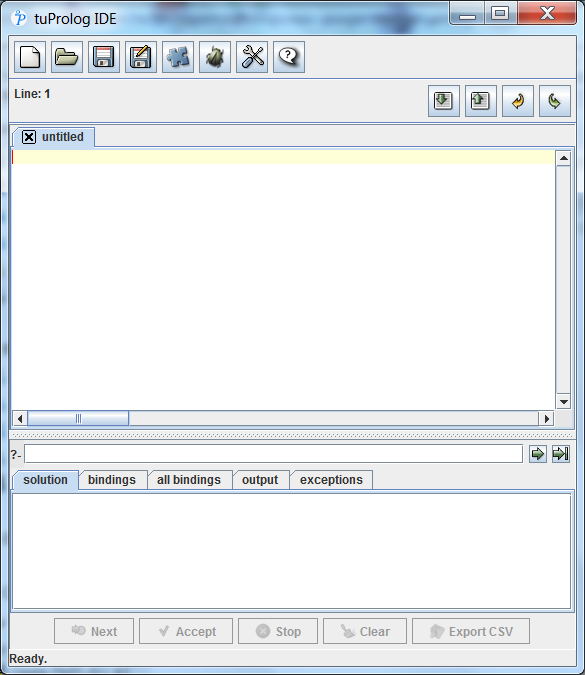
\includegraphics[scale=0.60]{images/tuPrologIDE}
\caption{\tuprolog\ IDE.}
\label{tuprolog-ide}
\end{figure}

The main window of the \tuprolog\ IDE is shown in \figref{tuprolog-ide}.
%
It is divided in two sections:
%
\begin{itemize}
\item an editing area on the middle, providing means to edit the engine's current theory;
\item a console on the bottom, providing means to ask queries and display their solutions.
\end{itemize}
%
In the main window there also are:
%
a toolbar at the top, providing facilities to manage theories, such as load, save as well as create a new theory, to load and unload libraries into and from the \tuprolog\ engine, and to view in a separate window the debug informations activated by means of the \predicate{spy/0} predicate;
%
and a status bar at the very bottom, providing status informations for the IDE and the engine.

\subsection{Editing the theory}

The editing area allows multiple theories to be created and modified at the same time, by allocating a tab with a new text area for each theory.
%
The text area provides syntax highlighting for comments, string and list literals, and predefined predicates.
%
Undo and Redo actions are supported through the usual \keycap{Ctrl}+\keycap{Z} and \keycap{Ctrl}+\keycap{Shift}+\keycap{Z} key bindings.

\begin{figure}
\centering
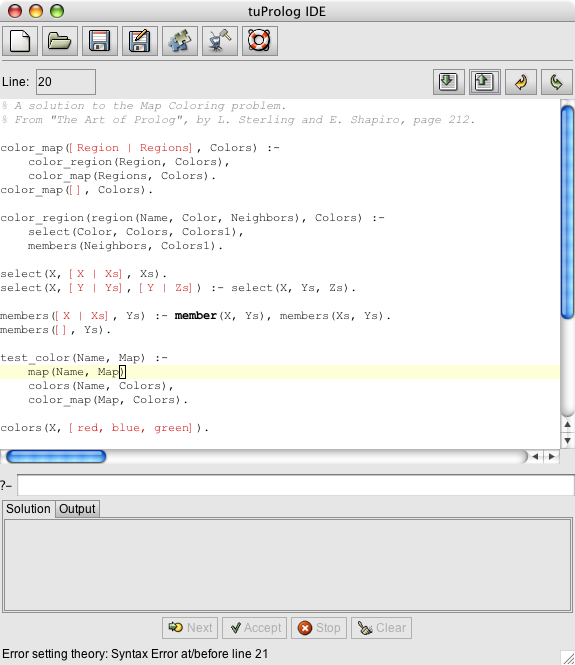
\includegraphics[scale=0.60]{images/syntaxErrorFound}
\caption{A syntax error is found when setting the content of the editor area as the new engine's theory.}
\label{syntax-error-found}
\end{figure}

\begin{figure}
\centering
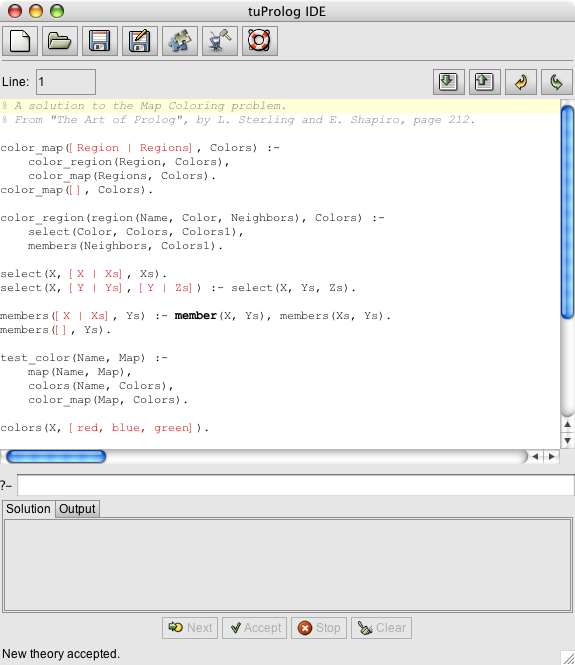
\includegraphics[scale=0.60]{images/setTheorySucceeded}
\caption{The syntax error is removed and the \guibutton{Set Theory} operation succeeds.}
\label{set-theory-succeeded}
\end{figure}

Above the editing tabs, a control area is found, where two buttons are provided to get the text of the engine's current theory into a new tab and to set the text contained in the editor of the selected tab as a new theory for the engine, and two buttons are provided for mouse-clicking support of Undo and Redo
actions.
%
An apposite action for retrieving the engine's current theory in an editor (shown in \figref{syntax-error-found}) is needed because whenever that theory gets modified by other means, such as calling the \texttt{consult/1} predicate, the changes are not automatically reflected in any text area.
%
On the left side of the control area, there also is an indicator of the line where the caret is currently positioned in the edit area.
%
Informations about the result of the action issued by the control area are provided in the status bar at the very bottom of the IDE's window:
%
for instance, when setting an invalid theory to the engine because of syntax errors, details about the error are provided.

\subsection{Solving goals}

The console at the bottom of the tuProlog IDE's window is subdivided in two logical panes:
%
\begin{itemize}
\item a query pane composed by a textfield where queries can be inserted, and two buttons to trigger the solving process.
%
The leftmost (\guibutton{Solve}) button asks the engine to find the first solution to the query, allowing the user to possibly navigate through further solutions;
%
the rightmost (\guibutton{Solve All}) button forces the engine to find all solutions to the given query.
%
Pressing the \keycap{Enter} key in the textfield has the same effect as pressing the \guibutton{Solve} button.
\item an answer pane, where answers and output informations are visualized.
%
Answers to Prolog queries are composed by both solutions, showed in a free form within a read-only text area, and bindings, displayed in tabular form.
%
The output tab provides a read-only view on the standard output where informations are possibly written by Prolog programs, by means of the I/O predicates supplied by the \classname{IOLibrary}.\footnote{The information written on standard output by methods invoked on Java objects from the \classname{JavaLibrary} -- for instance using the \varname{stdout} object -- are not displayed on this view.}
%
Control buttons are also provided to iterate through possibly multiple solutions, clear the bindings and output panes, and export tabular data in a convenient CSV format.
\end{itemize}
%
Goals are asked through the query input box, and answers (bindings and solutions) are provided in the related text area.
%
Query and answers are traced in a proper chronological history, that can be explored by means of \keycap{Up} and \keycap{Down} arrow keys from the query input textfield.
%
When open alternatives are found solving a goal, the \guibutton{Next} and \guibutton{Accept} buttons are enabled in the answer pane to interact with the engine, in order to let the user specify if the current solution is accepted or if other alternatives need to be explored.

Note that the theory contained in the currently selected edit pane does not have to be explicitly feeded to the Prolog engine before it could be possible to solve queries against that theory's knowledge base.
%
In fact, any time a goal is asked to be solved, the theory contained in the active edit area is automatically feeded to the engine if its knowledge base has been modified since the last solved goal.
%
(This obviously happens also on the first time a query is asked.)
%
However, whenever the engine's theory is modified by other means than the editor, it does need to be explicitly acquired and presented to the programmer in the text area.
%
In fact, if the theory in the engine is augmented by a call to the predicate \predicate{consult/1} issued from a query, for example, the contents of the newly consulted theory will not be automatically inserted in the editor:
%
when the programmer needs an up-to-date view of the knowledge base contained in the underlying \tuprolog\ engine, its display has to be explicitly triggered by means of the \guibutton{GetTheory} button, available
in the editing area.

An example of the user interaction involving multiple solutions is shown in the following sequence of figures:
%
in \figref{query-issued}, the user issued the query \userinput{test\_color(test, X).}, using the knowledge base written in the edit area (a solution to the Map Coloring problem,\footnote{The problem is to color a planar map so that no two adjoining regions have the same color. A famous conjecture was proved in 1976 showing that four colors are sufficient to color any planar map.} with a test map composed of six areas).
%
The first solution is displayed, and multiple open alternatives can be explored:
%
in \figref{next-solution-asked}, the user asked to get the next possible solution by pressing the \guibutton{Next} button, and another solution is provided;
%
finally, in \figref{accept-solution}, the user, after having explored the first two solutions, accepts the third one by pressing the \guibutton{Accept} button.
%
During the resolution of a goal, all the theory-related buttons are disabled, included the \guibutton{Library Manager} button, since each library can have its theory to be feeded into the engine.

\begin{figure}
\centering
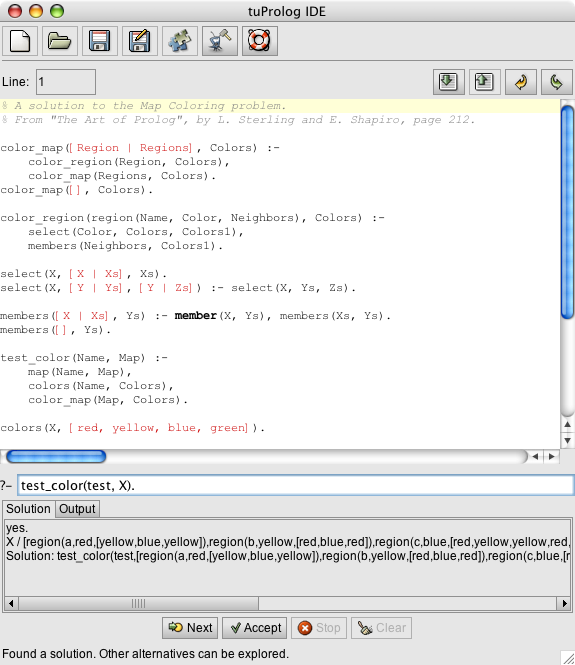
\includegraphics[scale=0.605]{images/queryIssued}
\caption{The user issued a query \userinput{test\_color(test, X).} and the first solution is displayed.}
\label{query-issued}
\end{figure}

\begin{figure}
\centering
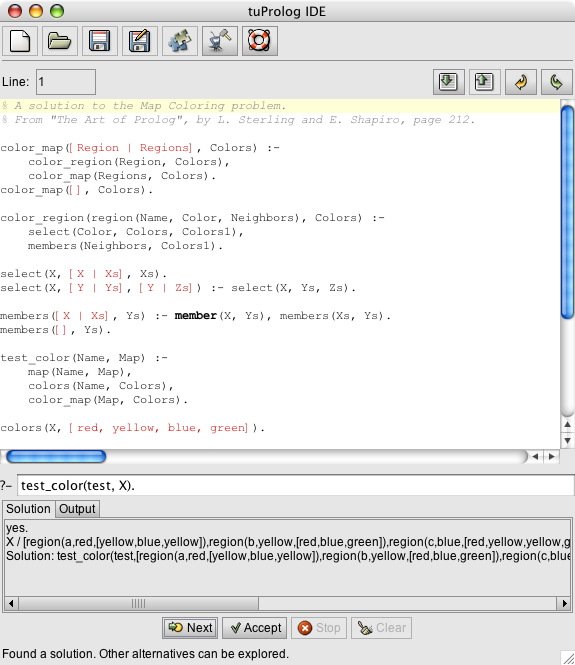
\includegraphics[scale=0.605]{images/nextSolutionAsked}
\caption{The user issued a \guibutton{Next} command and got another solution.}
\label{next-solution-asked}
\end{figure}

\begin{figure}
\centering
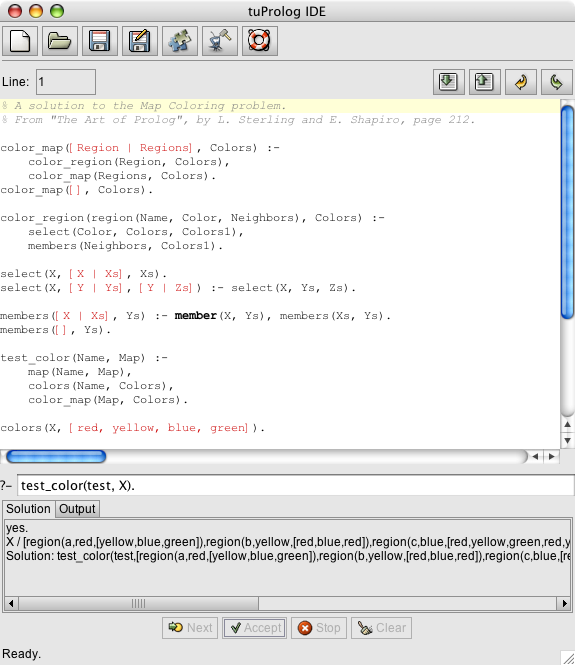
\includegraphics[scale=0.605]{images/acceptSolution}
\caption{The user accepted the third solution by pressing the \guibutton{Accept} button.}
\label{accept-solution}
\end{figure}

Near to the \guibutton{Next} and \guibutton{Accept} buttons, a \guibutton{Stop} button is found, providing the user with a means to halt the engine if a computation takes too long or a bug in the knowledge base feeded to the engine results in an infinite loop.

% Such a bug is contained in the following theory:
% \begin{verbatim}
% p(a).
% p(b) :- p(b).
% p(c).
% \end{verbatim}
% When solving a goal like \code{p(b)} or asking for the second solution to the query \code{p(X)}, the \tuprolog\ engine
% will be trapped in an infinite loop due to the particular recursive nature of the second clause in the feeded theory.
% By pressing the \guibutton{Stop} button, which is enabled only during computations, the user will be able to halt the
% engine and perform the necessary changes to the knowledge base before issuing another query, instead of being forced
% to close and reopen the IDE.

Finally, a \guibutton{Clear} button is provided, with the aim of allowing the user to clear the bindings and output panes when they get overfull with informations.
%
The button is enabled only when the proper tabs are selected.

\subsection{Debug Informations}

By pressing the \guibutton{View Debug Information} button, a new window is opened, providing a view on the warnings, produced by events such as the attempt at redefining a library predicate, and the spy information, concerning basic steps of the engine computation and state, possibly supplied by the engine during a goal demonstration:
%
Warnings are always active;
%
in order to activate the spy information notification, the \predicate{spy/0} built-in predicate (provided by \classname{BasicLibrary}) must be issued;
%
\predicate{nospy/0} can be used to stop this notification.
%
As an example, \figref{view-debug-information} shows the content of the spy information view after the
execution of a goal involving the activation of spy inspection.

It is worth noting that a computation may contain a huge number of traced steps.
%
For this reason, a toolbar at the top of the window allows to collapse and expand all nodes in the spy information pane, or to expand and collapse selected nodes only.
%
Finally, the content of the warnings and spy panes can be cleared using the \guibutton{Clear} button at the leftmost end of the toolbar.

\begin{figure}
\centering
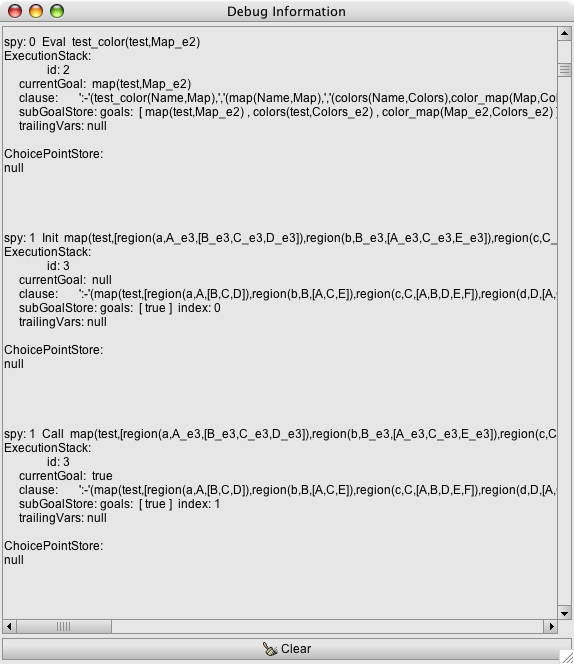
\includegraphics[scale=0.605]{images/viewDebugInformation}
\caption{Debug Information View after the execution of a goal.}
\label{view-debug-information}
\end{figure}

\subsection{Dynamic library management}


A \tuprolog\ engine can be extended by loading any number of libraries, each provinding a specific set of built-in
predicates and functors, and a related theory. The \tuprolog\ IDE allows a dynamic management of libraries through a
GUI dialog, which can be displayed by pressing the \guibutton{Open Library Manager} button in the toolbar. The Library
Manager dialog is shown in \figref{library-manager-dialog}.

\begin{figure}
\centering
\includegraphics[scale=0.605]{images/libraryManagerDialog}
\caption{The Library Manager dialog.}
\label{library-manager-dialog}
\end{figure}

This dialog displays a list of the libraries currently loaded into the \tuprolog\ engine. For a new instance of the
engine, that list will typically contain the four standard libraries coming with the application core, that is
\classname{BasicLibrary}, \classname{IOLibrary}, \classname{ISOLibrary}, \classname{JavaLibrary}, along with their
current status. The user can add a library to the Library Manager simply by providing the fully qualified name of the
library's class in the textfield on the top of the dialog, then pressing the \guibutton{Add} button: the added library
will be displayed with an initial Unload status. The user can further select the status of each library in the list,
and commit changes to the \tuprolog\ engine by pressing the \guibutton{OK} button, or dismiss the dialog by pressing
the \guibutton{Cancel} button.

The library manager is also capable of updating itself accordingly to the events of libraries load and unload fired by
the \tuprolog\ engine.  Such events are triggered by the use of the \verb|load_library/1| and \verb|unload_library/1|
predicates or directives in query issued or theories feeded to the engine. So, if an user asks to solve the goal \verb|load_library('TestLibrary'), test(X).|,
for example, the manager would immediately reflect the change occurred in the engine's libraries pool, adding a new
entry if \verb|TestLibrary| had not been previously loaded or, if necessary, changing the library's entry status to
show the result of the loading action.

Both the action of adding a library to the manager and the action of loading a library into the engine can fail. If,
for example, the classname provided does not identify a \tuprolog\ library (i.e. it identifies a class not extending the
\classname{alice.tuprolog.Library} class) or the identified class does not exist, an appropriate message will appear
in the status bar at the bottom of the dialog. When adding or loading a library, please remember that every class
needed by that library must be in the classpath in order to have the library correctly added to the manager's list or
loaded into the engine. 
%******************************************************************************%
%=======================================================================
\chapter{Using \tuprolog{} from Java}
\label{java-api}
%=======================================================================

\section{Getting started}

Let's begin with your first Java program using \tuprolog{}.
%
{\small{
\begin{verbatim}
    import alice.tuprolog.*;

    public class Test2P {
        public static void main(String[] args) throws Exception {
            Prolog engine = new Prolog();
            SolveInfo info = engine.solve("append([1],[2,3],X).");
            System.out.println(info.getSolution());
        }
    }
\end{verbatim}
}}
\noindent In this first example a \tuprolog{} engine is
created, and asked to solve a query, provided in a textual form.
%
This query in the Java environment is equivalent to the query\\\\
%
{\small{\texttt{?- append([1],[2,3],X).\\\\}}}
%
\noindent in a classic Prolog environment, and accounts for
finding the list that is obtained by appending the list
\texttt{[2,3]} to the list \texttt{[1]} (\texttt{append} is
included in the theory provided by the
\texttt{alice.tuprolog.lib.BasicLibrary}, which is downloaded by
the default when instantiating the engine).
%

By properly compiling and executing this simple program,\footnote{Save the program in a file called \texttt{Test2P.java}, then compile it with
%
\texttt{javac -classpath tuprolog.jar Test2P.java}
%
and then execute it with
%
\texttt{java -cp .;tuprolog.jar Test2P.java}} the string
\texttt{append([1],[2,3],[1,2,3])} -- that is the solution of out
query -- will be displayed on the standard output.
%
%

\noindent Then, let's consider a little bit more involved example:

{\small{
\begin{verbatim}
public class Test2P {
    public static void main(String[] args) throws Exception {
        Prolog engine = new Prolog();
        SolveInfo info = engine.solve("append(X,Y,[1,2]).");
        while (info.isSuccess()) {
            System.out.println("solution: " + info.getSolution() +
                               " - bindings: " + info);
            if (engine.hasOpenAlternatives()) {
                info = engine.solveNext();
            } else {
                break;
            }
        }
    }
}
\end{verbatim}
}}

In this case, all the solutions of a query are retrieved and
displayed, with also the variable bindings:
{\small{\begin{verbatim}

solution: append([],[1,2],[1,2]) - bindings: Y / [1,2]  X / []
solution: append([1],[2],[1,2]) - bindings: Y / [2]  X / [1]
solution: append([1,2],[],[1,2]) - bindings: Y / []  X / [1,2]

\end{verbatim}
}}

\section{Basic Data Structures}

\noindent All Prolog data objects are mapped onto Java objects:
\texttt{Term} is the base class for Prolog untyped terms such as
atoms and compound terms (represented by the \texttt{Struct} class),
Prolog variables (\texttt{Var} class) and Prolog typed terms such
as numbers (\texttt{Int}, \texttt{Long}, \texttt{Float},
\texttt{Double} classes).
%
In particular:

%
\begin{itemize}
    %
    \item \texttt{Term} -- this abstract class represents a generic Prolog term, and it is the
    root base class of \tuprolog{} data structures, defining the basic common services, such
    as term comparison, term unification and so on.
    %
    It is worth noting that it is an abstract class, so no direct \texttt{Term}
    objects can be instantiated;
    %
    %
    %
    \item \texttt{Var} -- this class (derived from \texttt{Term})
    represents \tuprolog{} variables.
    %
    A variable can be anonymous, created by means of the default constructor, with no
    arguments, or identified by a name, that must starts with an upper case letter or an
    underscore;
    %
    \item \texttt{Struct} -- this class (derived from \texttt{Term})
    represents un-typed \tuprolog{} terms, such as atoms, lists and compound terms;
    %
    \texttt{Struct} objects are characterised by a functor name and a
    list of arguments (which are \texttt{Term}s themselves), while
    \texttt{Var} objects are labelled by a string representing the
    Prolog name.
    %
    Atoms are mapped as \texttt{Struct}s with functor with a name and
    no arguments;
    %
    Lists are mapped as \texttt{Struct} objects with functor
    \verb|'.'|, and two \texttt{Term} arguments (head and tail of the list);
    %
    lists can be also built directly by exploiting the 2-arguments constructor, with
    head and tail terms as arguments.
    %
    Empty list is constructed by means of the no-argument constructor of \texttt{Struct}
    (default constructor).
    %
    \item \texttt{Number} -- this abstract class represents typed, numerical Prolog terms,
        and it is the  base class of \tuprolog{} number classes;
    %
    \item \texttt{Int, Long, Double, Float} -- these classes (derived from \texttt{Number})
    represent  typed numerical \tuprolog{} terms, respectively integer, long, double and
    float numbers.
    %
    Following the Java conventions, the default type for integer number is \texttt{Int}
    (integer, not long, number), and for \texttt{Double} (and so double), for floating point
    number.
\end{itemize}


\noindent Some examples of term creation follow:
%
{\small{\begin{verbatim}

// constructs the atom vodka
Struct drink = new Struct("vodka");

// constructs the number 40
Term degree = new alice.tuprolog.Int(40);

// constructs the compound degree(vodka, 40)
Term drinkDegree = new Struct("degree",
                              new Struct("vodka"),
                              new Int(40));
// second way to constructs the compound degree(vodka,40)
Struct drinkDegree2 = new Struct("degree", drink, degree);

// constructs the compound temperature('Rome', 25.5)
Struct temperature = new Struct("temperature",
                                new Struct("Rome"),
                                new alice.tuprolog.Float(25.5));

// constructs the compound equals(X, X)
Struct t1 = new Struct("equals", new Var("X"), new Var("X"));
t1.resolveTerm();

// mother(John,Mary)
Struct father = new Struct(new Struct("John"), new Struct("Mary")));

// father(John, _)
Term  father = new Struct(new Struct("John"), new Var());

// p(1, _, q(Y, 3.03, 'Hotel'))
Term  t2 = new Struct("p",
                      new Int(1),
                      new Var(),
                      new Struct("q",
                                 new Var("Y"),
                                 new Float(3.03f),
                                 new Struct("Hotel")));

// The Long number 130373303303
Term t3 = new alice.tuprolog.Long(130373303303h);

// The double precision number 1.7625465346573
Term t4 = new alice.tuprolog.Double(1.7625465346573);

// an empty list
Struct empty = new Struct();

// the list [303]
Struct l = new Struct(new Int(303), new Struct());

// the list [1,2,apples]
Struct alist = new Struct(
                   new Int(1),
                   new Struct(
                       new Int(2),
                       new Struct("apples")));

// fruits([apple, orange | _ ])
Term list2 = new Struct("fruits", new Struct(
                                      new Struct("apple",
                                          new Struct("orange"),
                                          new Var())));

// complex_compound(1, _, q(Y, 3.03, 'Hotel', k(Y,X)), [303, 13, _, Y])
Term t5 = Term.parse(
     "complex_compound(1, _, q(Y, 3.03, 'Hotel', k(Y,X)), [303, 13, _, Y])"
);

\end{verbatim}}}
%
\noindent The name of the \tuprolog{} number classes
(\texttt{Int}, \texttt{Float}, \texttt{Long}, \texttt{Double})
follows the name of the primitive Java data type they represents.
%
Note that due to class name clashes (for instance between classes
\texttt{java.lang.Long} and \texttt{alice.tuprolog.Long}), it
could be necessary to use the full class name to identify
\tuprolog{} classes.
%

\section{Engine, Theories and Libraries}

\noindent Then, the other main classes that make \tuprolog{} Core
API concern \tuprolog{} engines, theories and libraries. In
particular:
%
\begin{itemize}
    \item \texttt{Prolog} -- this class represent \tuprolog{}
    engines.
    %
    This class provides a minimal interface that enables users
    to: \\
    %
    \indent{-- set/get the theory to be used for
    demonstrations;}\\
        %
    \indent{-- load/unload libraries;} \\
        %
    \indent{-- solve a goal, represented either by a \texttt{Term} object or by a
        textual representation (a \texttt{String} object) of a
        term.}\\
    %
    A \tuprolog{} engine can be instantiated either with some standard default
    libraries loaded, by means of the default constructor, or with
    a starting set of libraries, which can be empty, provided as
    argument to the constructor (see JavaDoc documentation for
    details).
    %
    Accordingly, a raw, very lightweight, \tuprolog{} engine can
    be created by specifying an empty set of library, providing
    natively a very small set of built-in primitives.


    \item \texttt{Theory} -- this class represent \tuprolog{}
    theories.
    %
    A theory is represented by a text, consisting of a series of
    clauses and/or directives, each followed by a dot and a
    whitespace character.
    %
    Instances of this class are built either from a textual representation,
    directly provided as a string or taken by any possible input
    stream, or from a list of terms representing Prolog clauses.
    %
    %
    %
    %
    %
    \item \texttt{Library} -- this class represents \tuprolog{}
    libraries;
    %
    A \texttt{tuprolog} engine can be dynamically extended by loading
    (and unloading) any number of libraries; each library can provide
    a specific set of of built-ins predicates, functors and a related
    theory.
    %
    A library can be loaded by means of the built-in by means of the method
    \texttt{loadLibrary} of the \tuprolog{} engine.
    %
    Some standard libraries are provided in the
    \texttt{alice.tuprolog.lib} package and loaded by the default
    instantiation of a \tuprolog{} engine:
    %
    \texttt{alice.tuprolog.lib.BasicLibrary}, providing basic and
    well-known Prolog built-ins, \texttt{alice.tuprolog.lib.IOLibrary}
    providing \textit{de facto} standard Prolog I/O predicates, \texttt{alice.tuprolog.lib.ISOLibrary}
    providing some ISO predicates/functors not directly provided
    by \texttt{BasicLibrary} and \texttt{IOLibrary}, and
    \texttt{alice.tuprolog.lib.JavaLibrary}, which enables the
    creation and usage of Java objects from \tuprolog{} programs,
    in particular enabling the reuse of any existing Java resources.
    %
    %
    \item \texttt{SolveInfo} -- this class represents the result of a
    demonstration and instances of these class are returned by the
    \texttt{solve} methods the \texttt{Prolog} engines;
    %
    in particular \texttt{SolveInfo} objects provide services to test the
    success of the demonstration (\texttt{isSuccess} method),
    to access to the term solution of the query
    (\texttt{getSolution} method)  and to access the list of the
    variable with their bindings.
\end{itemize}
%

Some notes about \tuprolog{} terms and the services they provide:
\begin{itemize}
%
\item the static \texttt{parse} method provides a quick way to get a
term from its string representation.
%
\item \tuprolog{} terms provides directly methods for unification and matching: \\
%
{\tt{\small{public boolean unify(Term t)}}}\\
%
{\tt{\small{public boolean match(Term t)}}}\\
%
Terms that have been subject to unification outside a
demonstration context (that is invoking directly these methods,
and not passing through the solving service of an engine) should
not be used then in queries to engines.
%
\item some services are provided to compare terms, according to the
Prolog rules, and to check their type;
%
in particular the standard Java method \texttt{equals} has the
same semantics of the method \texttt{isEqual} which follows the
Prolog comparison semantics.
%
\item some services makes it possible to copy a term as it is
or to get a renamed copy of the term (\texttt{copy} and
\texttt{getRenamedCopy});
%
it is worth noting that the design of \tuprolog{} promotes a
stateless usage of terms; in particular, it is good practice not
to reuse the same terms in different demonstration contexts, as
part of different queries.
%
\item the method \texttt{getTerm} is useful in the case of
variables, providing the term linked possibly considering all the
linking chain in the case of variables referring other variables.
%
\item when a term is created by means of the proper constructor,
consider as example: \\\\
%
{\tt{\scriptsize{Struct myTerm = new Struct("p", new Var("X"), new
Int(1), new Var("X"))}}}\\\\
%
it is \emph{not resolved}, in the sense that possible variable
terms with the same name in the term do not refer each other;
%
so in the example the first and the third argument of the compound
\texttt{myTerm} point to different variable objects.
%
A term is resolved the first time it is involved in a matching or
unification context.
%
\end{itemize}

\noindent Some notes about \tuprolog{} engines, theories,
libraries and the services they provide:

\begin{itemize}
%
\item \tuprolog{} engines support natively some
\emph{directives}, that can be defined by means of the :-/1
predicate in theory specification.
%
Directives are used to specify properties of clauses and of the
engine (\emph{solve/1}, \emph{initialization/1},
\emph{set\_prolog\_flag/1}, \emph{load\_library/1},
\emph{consult/1}), format and syntax of read-terms (\emph{op/3},
\emph{char\_conversion/2}).
%
\item \tuprolog{} engines support natively the dynamic definition
and management of \emph{flags} (or property), used to describe
some aspects of libraries and their built-ins.
%
A flag is identified by a name (an alphanumeric atom), a list of
possible values, a default value and a boolean value specifying if
the flag value can be modified.
%
\item \tuprolog{} engines are thread-safe. The methods that could
create problems in being used in a multi-threaded context are now
synchronised.
%
\item \tuprolog{} engines have no (static) dependencies with each
other, multiple engines can be created independently as simple
objects on the same Java virtual machine,  each with its own
configuration (theory and loaded libraries).
%
Moreover, accordingly to the design of \tuprolog{} system in
general, engines are very lightweight, making suitable the use of
multiple engines in the same execution context.
%
\item \tuprolog{} engines can be serialised and stored as a persistent
object or sent through the network.
%
This is true also for engines with pre-loaded standard libraries:
%
in the case that other libraries are loaded, these must be
serializable in order to have the engine serializable.
%
\end{itemize}

%
%

\section{Some more examples of \tuprolog{} usage}

\noindent Creation of an engine (with default libraries
pre-loaded):

{\tt\scriptsize{
\begin{verbatim}
    import alice.tuprolog.*;

    ...
    Prolog engine = new Prolog();
\end{verbatim} }}


\noindent Creation of an engine specifying only the
\texttt{BasicLibrary} as pre-loaded library:

{\tt\scriptsize{
\begin{verbatim}
    import alice.tuprolog.*;

    ...
    Prolog engine = new Prolog(new String[]{"alice.tuprolog.lib.BasicLibrary"});
\end{verbatim} }}

\noindent Creation and loading of a theory from a string:

{\tt\scriptsize{\begin{verbatim}

    String theoryText = "my_append([],X,X).\n" +
                        "my_append([X|L1],L2,[X|L3]) :- my_append(L1,L2,L3).\n";

    Theory theory = new Theory(theoryText);
    try {
        engine.setTheory(theory);
    } catch(InvalidTheoryException e) {
    }
\end{verbatim} }}

\noindent Creation and loading of a theory from an input stream:

{\tt\scriptsize{\begin{verbatim}

    Theory theory = new Theory(new FileInputStream("test.pl");
    try {
        engine.setTheory(theory);
    } catch(InvalidTheoryException e) {
    }
\end{verbatim} }}

\noindent Goal demonstration (provided as a string):

{\tt\scriptsize{\begin{verbatim}

    // ?- append(X,Y,[1,2,3]).
    try {
        SolveInfo info = engine.solve("append(X,Y,[1,2,3]).");
        Term solution = info.getSolution();
    } catch(MalformedGoalException mge) {
        ...
    } catch(NoSolutionException nse) {
        ...
    }
\end{verbatim} }}

\noindent Goal demonstration (provided as a Term):

{\tt\scriptsize{\begin{verbatim}

    try {
        Term goal = new Struct("p", new Int(1), new Var("X"));
        try {
            // ?- p(1,X).
            SolveInfo info = engine.solve(goal);
            Term solution = info.getSolution();
 
        } catch (NoSolutionException nse) {
        }
    } catch (InvalidVarNameException ivne) {
    }
\end{verbatim} }}

\noindent Getting another solution:

{\tt\scriptsize{\begin{verbatim}
    try {
        SolveInfo info = engine.solve(goal);
        info = engine.solveNext();
    } catch(NoMoreSolutionException e)
\end{verbatim} }}

\noindent Loading a library:

{\tt\scriptsize{\begin{verbatim}
    try {
        engine.loadLibrary('alice.tuprologx.lib.TucsonLibrary');
    } catch(InvalidLibraryException e) {
    }
\end{verbatim} }}

\noindent Here, a complete example of interaction with a
\tuprolog{} engine is shown (refer to the JavaDoc documentation for
details about interfaces):

{\tt\scriptsize{\begin{verbatim}

import alice.tuprolog.*; import java.io.*;

public class Test2P {
    public static void main (String args[]) {
        Prolog engine = new Prolog();
        try {

            // solving a goal
            SolveInfo info = engine.solve(new Struct("append",
                                              new Var("X"),
                                              new Var("Y"),
                                              new Struct(new Term[]{new Struct("hotel"),
                                                                    new Int(303),
                                                                    new Var()})));


            // note we could use strings:
            // SolveInfo info = engine.solve("append(X, Y, [hotel, 303, _]).");

            // test for demonsration success
            if (info.isSuccess()) {

                // acquire solution and substitution
                Term sol = info.getSolution();
                System.out.println("Solution: " + sol);

                System.out.println("Bindings: " + info);

                // open choice points?
                if (engine.hasOpenAlternatives()) {

                    // ask for another solution
                    info = engine.solveNext();

                    if (info.isSuccess()) {
                        System.out.println("An other substitution: " + info);
                    }
                }
            }

            // other frequent interactions

            // setting a new theory in the engine
            String theory = "p(X,Y) :- q(X), r(Y).\n" +
                            "q(1).\n" +
                            "r(1).\n" +
                            "r(2).\n";
            engine.setTheory(new Theory(theory));

            SolveInfo info2 = engine.solve("p(1,X).");
            System.out.println(info2);

            // retrieving the theory from a file
            FileOutputStream os=new FileOutputStream("test.pl");
            os.write(theory.getBytes());
            os.close();
            engine.setTheory(new Theory(new FileInputStream("test.pl")));
            info2 = engine.solve("p(X,X).");
            System.out.println(info2.getSolution());

        } catch (Exception ex) {
            ex.printStackTrace();
        }
    }
}
\end{verbatim}}}

With the program execution, the following string are displayed on
the standard output:

{\tt\small{

\begin{verbatim}
Solution: append([],[hotel,303,_],[hotel,303,_])
Bindings: Y /[hotel,303,_] X / []
An other substitution: Y / [303,_]  X / [hotel]
X / 1
p(1,1)
\end{verbatim}}}
%******************************************************************************%
%=======================================================================
\chapter{How to Develop New Libraries}
\label{ch:howto-develop-libraries}
%=======================================================================

Libraries are \tuprolog{}'s way to achieve the desired characteristics
of minimality, dynamic configurability, and straightforward
Prolog-to-Java integration.
%
Libraries are reflection-based, and can be written both in Prolog
and Java: other languages may be used indirectly, via JNI (Java
Native Interface).
%
At the \tuprolog{} side, exploiting a library written in Java
requires no pre-declaration of the new built-ins, nor any other
special mechanism: all is needed is the presence of the
corresponding \texttt{.class} library file in the proper location
in the file system.

\section{Implementation details}

Syntactically, a library developed in Java must extend the base
abstract class \texttt{alice.tuprolog.Library}, provided within
the \tuprolog{} package, and define new \textit{predicates} and/or
\textit{evaluable functors} and/or \textit{directives} in the form
of methods, following a simple signature convention.
%
In particular, new predicates must adhere to the signature:
%
\begin{center}
\small\tt
    public boolean <\textit{pred name}>\_<\textit{N}>(\textit{T1} arg1,
\textit{T2} arg2, ...,\textit{Tn} argN)
\end{center}
%
while evaluable functors must follow the form:
%
\begin{center}
    \small\tt
    public Term <\textit{eval funct name}>\_<\textit{N}>(\textit{T1} arg1,
\textit{T2} arg2, ...,\textit{Tn} argN)
\end{center}
%
and directives must be provided with the signature:
%
\begin{center}
    \small\tt
    public void <\textit{dir name}>\_<\textit{N}>(\textit{T1} arg1,
\textit{T2} arg2, ..., \textit{Tn} argN)
\end{center}
%
where \textit{T1}, \textit{T2}, ... \textit{Tn} are \texttt{Term} or derived
classes, such as \texttt{Struct}, \texttt{Var}, \texttt{Long}, etc., defined in
the \tuprolog{} package, constituting  the Java counterparts of
the corresponding Prolog data types.
%
The parameters represent the arguments actually passed to the built-in
predicate, functor, or directive.

%
A library defines also a new piece of theory, which is collected
by the Prolog engine through a call to the library method \texttt{String
getTheory()}.
%
By default, this method returns an empty theory: libraries which need to
add a Prolog theory must override it accordingly.
%
Note that only the external representation of a library's theory is
constrained to be in \texttt{String} form; the internal implementation
can be freely chosen by the library designer. However, using a Java
\texttt{String} for wrapping a library's Prolog code guarantees
self-containment while loading libraries through remote mechanisms such
as RMI.

\begin{table}[h]
    %
    \caption{Predicate and functor definitions in Java and their use
    in a \tuprolog{} program.\labeltab{java-preds}}
    %
    \begin{center}{\small\tt
    \begin{tabular}{p{10cm}|p{3.25cm}}
     \hline
     & \\
    \textit{// sample library} & \textit{\% tuProlog test program}\\
     import alice.tuprolog.*; & \\
     & \\
    public class TestLibrary extends Library \{                            &
 test :-\\
    ~~\textit{// builtin functor sum(A,B)}                          & ~~N is sum(5,6),\\
    ~~public Term sum\_2(Number arg0, Number arg1)\{    & ~~println(N).\\
    ~~~~float   arg0 = arg0.floatValue();        & \\
    ~~~~float   arg1 = arg1.floatValue();        & \\
    ~~~~return new Float(arg0+arg1);                                & \\
    ~~\}                                                            & \\
    ~~\textit{// builtin predicate println(Message)}                & \\
    ~~public boolean println\_1(Term arg)\{                      & \\
    ~~~~System.out.println(arg);                                   & \\
    ~~~~return true;                                                & \\
    ~~\}                                                            & \\
    \}                                                              & \\
     & \\
     \hline
    \end{tabular}
    }\end{center}
\end{table}

\xt{java-preds} shows a couple of examples about how a predicate
(such as \texttt{println/1}) and an evaluable functor (such as
\texttt{sum/2}) can be defined in Java and exploited from
\tuprolog{}.
%
The Java method \texttt{sum\_2}, which implements the evaluable
functor \texttt{sum/2}, is passed two \texttt{Number} terms (5 and 6)
which are then used (via \texttt{getTerm}) to retrieve the two
(float) arguments to be summed.
%
In the same way, method \texttt{println\_1}, which implements the
predicate \texttt{println/1}, receives \texttt{N} as \texttt{arg},
and retrieves its actual value via \texttt{getTerm}: since this is
a predicate, a boolean value (\texttt{true} in this case) is returned.
%

The developer of a library may face two corner case as far as method
naming is concerned: the first happens when the name of the
predicate, functor or directive she is defining contains a symbol
which cannot legally appear in a Java method's name; the second
occurs when he has to define a predicate and a directive with the
same Prolog signature, which Java would not be able to tell apart
because it cannot distinguish signatures of methods differing for
their return type only.
%
To overcome this kind of issues, a {\em synonym map} can be
constructed under the form of an array of \texttt{String} arrays,
and returned by the appropriate \texttt{getSynonymMap} method,
defined as abstract by the \texttt{Library} class. In both the cases
described above, another name must be chosen for the Prolog
executable element the library's developer want to define: then, by
means of the synonym map, that fake name can be associated with the
real name and the type of the element, be it a predicate, a functor
or a directive.
%
For example, if a definition for an evaluable functor representing
addition is needed, but the symbol \texttt{+} cannot appear in a
Java method's name, a method called \texttt{add} can be defined and
associated to its original Prolog name and its function by inserting
the array \texttt{\{"+", "add", "functor"\}} in the synonym map.

\section{Library Name}

% Lib name
%
By default, the name of the library coincides with the full class name of the
class implementing it.
%
However, it is possible to define explicitly the name of a library by
overriding the \texttt{getName} method, and returning as a string
the real name.
%
For example:
%
\begin{verbatim}
package acme;
import alice.tuprolog.*;
public class MyLib_ver00 extents Library {
    public String getName(){
        return "MyLibrary";
    }
    ...
}
\end{verbatim}

This class defines a library called \texttt{MyLibrary}.
%
It can be loaded into a Prolog engine by using the
\texttt{loadLibrary} method on the Java side, or a
\texttt{load\_library} built-in predicate on the Prolog side,
specifying the full class name (\texttt{acme.MyLib\_{ve00}}).
%
It can be unloaded then dynamically using the \texttt{unloadLibrary}
method (or the corresponding \texttt{unload\_library} built-in),
specifying instead the \textit{library name} (\texttt{MyLibrary}).

%******************************************************************************%
%=======================================================================
\chapter{\tuprolog{} Exceptions}
ss\label{ch:exceptions}
%=======================================================================

%=======================================================================
\section{Exceptions in ISO Prolog}
\label{sec:exceptions in ISO prolog}
%=======================================================================
Exception handling was first introduced in the ISO Prolog standard (ISO/IEC 13211-1) in 1995.

The first distinction has to be made between \textit{errors} and \textit{exceptions}.
%
An \textit{error} is a particular circumstance that interrupts the execution of a Prolog program: when a Prolog engine encounters an error, it raises an \textit{exception}.
%
The exception handling support is supposed to intercept the exception and transfer the execution flow to a suitable exception handler, with any relevant information. Two basic principles are followed during this operation:

\begin{itemize}
  \item \textit{error bounding} -- an error must be bounded and not propagate through the entire program: in particular, an error occurring inside a given component must either be captured at the component's frontier, or remain invisible and be reported nicely.
      According to ISO Prolog, this is done via the \texttt{catch/3} predicate.

  \item \textit{atomic jump} -- the exception handling mechanism must be able to exit atomically from any number of nested execution contexts. According to ISO Prolog, this is done via the \texttt{throw/1} predicate.
\end{itemize}
%
In practice, the \texttt{catch(\textit{Goal}, \textit{Catcher}, \textit{Handler})} predicate enables the controlled execution of a goal, while the \texttt{throw(\textit{Error})} predicates makes it possible to raise an exception---very much like the \texttt{try/catch} construct of many imperative languages.

Semantically, executing the \texttt{catch(\textit{Goal}, \textit{Catcher}, \textit{Handler})} means that \texttt{\textit{Goal}} is first executed: if an error occurs, the subgoal where the error occurred is replaced by the corresponding \texttt{throw(\textit{Error})}, which raises the exception.
%
Then, a matching \texttt{catch/3} clause -- that is, a clause whose second argument
unifies with \texttt{\textit{Error}} -- is searched among the ancestor nodes in the resolution tree: if one is found, the path in the resolution tree is cut, the catcher itself is removed (because it only applies to the protected goal, not to the handler), and the \texttt{\textit{Handler}} predicate is executed. If, instead, no such matching clause is found, the execution simply fails.

So, \texttt{catch(\textit{Goal}, \textit{Catcher}, \textit{Handler})} performs exactly like \texttt{\textit{Goal}} if no exception are raised: otherwise, all the choicepoints generated by \texttt{\textit{Goal}} are cut, a matching \texttt{\textit{Catcher}} is looked for, and if one is found \texttt{\textit{Handler}} is executed, maintaining the substitutions made during the previous unification process.
%
Then, execution continues with the subgoal following \texttt{catch/3}.
%
Any side effects possibly occurred during the execution of a goal are \textit{not} undone in case of exceptions---as it normally happens when a predicate fails.

Summing up, \texttt{catch/3} succeeds if:
\begin{itemize}
  \item \texttt{call(\textit{Goal})} succeeds \textit{(standard behaviour)};\\\\
        --OR--
  \item \texttt{call(\textit{Goal})} is interrupted by a call to
      \texttt{throw(\textit{Error})} whose \texttt{\textit{Error}} unifies with
      \texttt{\textit{Catcher}}, and the subsequent \texttt{call(\textit{Handler})} succeeds.
\end{itemize}

\noindent If \texttt{\textit{Goal}} is non-deterministic, it can be executed again in
backtracking. However, since all the choicepoints of \texttt{\textit{Goal}} are cut in case of exception, \texttt{\textit{Handler}} \textit{is possibly executed just once}.

\smallskip

\noindent As an example, let us consider the following toy program:
\begin{verbatim}
    p(X):- throw(error), write('---').
    p(X):- write('+++').
\end{verbatim}

\noindent with the following query:

\begin{verbatim}
    ?:- catch(p(0), E, write(E)), fail.
\end{verbatim}
which tries to execute \texttt{p(0)}, catching any exception \texttt{E} and handling the error by just printing it on the standard output (\texttt{write(E)}).

Perhaps surprisingly, the program will just print \texttt{'error'}, not \texttt{'error---'} or \texttt{'error+++'}. The reason is that once the exception is raised, the execution of \texttt{p(X)} is aborted, and after the handler terminates the execution proceeds with the subgoal following \texttt{catch/3}, i.e. \texttt{fail}.
So, \texttt{write('---')} is never reached, nor is \texttt{write('+++')} since all the choicepoints are cut upon exception.

%-----------------------------------------------------------------------
\subsection{Error classification}
%-----------------------------------------------------------------------
This classification was already presented in Section \ref{sec:exception-support} above as a hint to predicate and functor readability: however, we report it here too both for completeness and for the reader's convenience.

When an exception is raised, the relevant error information is also transferred by instantiating a suitable \textit{error term}.

The ISO Prolog standard prescribes that such a term follows the pattern
\texttt{error(\textit{Error\_term}, \textit{Implementation\_defined\_term})} where
\texttt{\textit{Error\_term}} is constrained by the standard to a pre-defined set of values (the error categories), and \texttt{\textit{Implementation\_defined\_term}} is an optional term providing implementation-specific details.
%
Ten error categories are defined:
\begin{enumerate}
  \item \texttt{instantiation\_error}: when the argument of a predicate or one of its components is an unbound variable, which should have been instantiated. Example: \texttt{X is Y+1} when \texttt{Y} is not instantiated at the time \texttt{is/2} is evaluated.

  \item \texttt{type\_error(\textit{ValidType}, \textit{Culprit})}: when the type of an argument of a predicate, or one of its components, is instantiated, but is bound to the wrong type of data. \texttt{\textit{ValidType}} represents the expected data type (one of \texttt{atom}, \texttt{atomic}, \texttt{byte}, \texttt{callable}, \texttt{character}, \texttt{evaluable}, \texttt{in\_byte}, \texttt{in\_character}, \texttt{integer}, \texttt{list}, \texttt{number}, \texttt{predicate\_indicator}, \texttt{variable}), and \texttt{\textit{Culprit}} is the actual (wrong) type found.
      Example: a predicate expecting months to be represented as integers in the range 1--12 called with an argument like \texttt{march} instead of \texttt{3}.

  \item \texttt{domain\_error(\textit{ValidDomain}, \textit{Culprit})}: when the argument type is correct, but its value falls outside the expected range.
      \texttt{\textit{ValidDomain}} is one of \texttt{character\_code\_list},
      \texttt{not\_empty\_list}, \texttt{not\_less\_than\_zero}, \texttt{close\_option}, \texttt{io\_mode}, \texttt{operator\_priority}, \texttt{operator\_specifier}, \texttt{flag\_value}, \texttt{prolog\_flag}, \texttt{read\_option}, \texttt{write\_option}, \texttt{source\_sink}, \texttt{stream}, \texttt{stream\_option}, \texttt{stream\_or\_alias}, \texttt{stream\_position},\\
      \texttt{stream\_property}. Example: a predicate expecting months as above, called with an out-of-range argument like \texttt{13}.

  \item \texttt{existence\_error(\textit{ObjectType}, \textit{ObjectName}}): when the referenced object does not exist. \texttt{\textit{ObjectType}} is
      the type of the unexisting object (one of \texttt{procedure}, \texttt{source\_sink}, or \texttt{stream}), and \texttt{\textit{ObjectName}} is the missing object's name. Example: trying to access an unexisting file like \texttt{usr/goofy} leads to an
      \texttt{existence\_error(stream, 'usr/goofy')}.

  \item \texttt{permission\_error(\textit{Operation}, \textit{ObjectType}, \textit{Object})}: whenever\\
       \texttt{\textit{Operation}} (one of \texttt{access}, \texttt{create}, \texttt{input}, \texttt{modify}, \texttt{open}, \texttt{output}, or \texttt{reposition}) is not allowed on \texttt{\textit{Object}}, of type \texttt{\textit{ObjectType}} (one of  \texttt{binary\_stream}, \texttt{past\_end\_of\_stream}, \texttt{operator}, \texttt{private\_procedure}, \texttt{static\_procedure}, \texttt{source\_sink}, \texttt{stream}, \texttt{text\_stream}, \texttt{flag}).

  \item \texttt{representation\_error(\textit{Flag})}: when an implementation-defined limit, whose category is given by \texttt{\textit{Flag}} (one of
      \texttt{character}, \texttt{character\_code}, \texttt{in\_character\_code}, \texttt{max\_arity}, \texttt{max\_integer}, \texttt{min\_integer}), is violated during execution.

  \item \texttt{evaluation\_error(\textit{Error})}: when the evaluation of a function produces an out-of-range value (one of \texttt{float\_overflow}, \texttt{int\_overflow}, \texttt{undefined}, \texttt{underflow}, \texttt{zero\_divisor}).

  \item \texttt{resource\_error(\textit{Resource})}: when the Prolog engine does not have enough resources to complete the execution of the goal. \texttt{Resource} can be any term useful to describe the situation. Examples: maximum number of opened files reached, no further available memory, etc.

  \item \texttt{syntax\_error(\textit{Message})}: when data read from an external source have an incorrect format or cannot be processed for some reason. \texttt{\textit{Message}} can be any term useful to describe the situation.

  \item \texttt{system\_error}: any other unexpected error not falling into the previous categories.
\end{enumerate}

%=======================================================================
\section{Exceptions in \tuprolog}
\label{sec:exceptions in tuprolog}
%=======================================================================

\tuprolog{} aims to fully comply to ISO Prolog exceptions.
%
In the following, a set of mini-examples are presented which highlight each one single aspect of \tuprolog{} compliance to the ISO standard.

%-----------------------------------------------------------------------
\subsection{Examples}
%-----------------------------------------------------------------------

\medskip\noindent
\textit{\textbf{Example 1:} \texttt{Handler} must be executed maintaining the substitutions made during the unification process between \texttt{Error} and \texttt{Catcher}}

Program: \texttt{p(0) :- throw(error).}

Query: \texttt{ ?- catch(p(0), E, atom\_length(E, Length)).}

Answer: \texttt{ yes.}

Substitutions: \texttt{E/error}, \texttt{Length/5}


\medskip\noindent
\textit{\textbf{Example 2:} the selected \texttt{Catcher} must be the nearest in the resolution tree whose second argument unifies with \texttt{Error}}

Program: \texttt{p(0) :- throw(error).}\\
\mbox{\texttt{~~~~~~~~~~~}}\texttt{p(1).}

Query: \texttt{ ?- catch(p(1), E, fail),  catch(p(0), E, true).}

Answer: \texttt{ yes.}

Substitutions: \texttt{E/error}


\medskip\noindent
\textit{\textbf{Example 3:} execution must fail if an error occurs during a goal execution and there is no matching \texttt{catch/3} predicate whose second argument unifies with \texttt{Error}}

Program: \texttt{p(0) :- throw(error).}

Query: \texttt{ ?- catch(p(0), error(X), true).}

Answer: \texttt{ no.}


\medskip\noindent
\textit{\textbf{Example 4:} execution must fail if \texttt{Handler} is false}

Program: \texttt{p(0) :- throw(error).}

Query: \texttt{ ?- catch(p(0), E, false).}

Answer: \texttt{ no.}


\medskip\noindent
\textit{\textbf{Example 5:} if \texttt{Goal} is non-deterministic, it is executed again on backtracking, but in case of exception all the choicepoints must be cut, and \texttt{Handler} must be executed only once}

Program: \texttt{p(0).}\\
\mbox{\texttt{~~~~~~~~~~~}}\texttt{p(1) :- throw(error).}\\
\mbox{\texttt{~~~~~~~~~~~}}\texttt{p(2).}

Query: \texttt{ ?- catch(p(X), E, true).}

Answer: \texttt{ yes.}

Substitutions: \texttt{X/0}, \texttt{E/error}

Choice: \texttt{ Next solution?}

Answer: \texttt{ yes.}

Substitutions: \texttt{X/1}, \texttt{E/error}

Choice: \texttt{ Next solution?}

Answer: \texttt{ no.}


\medskip\noindent
\textit{\textbf{Example 6:} execution must fail if an exception occurs in \texttt{Handler}}

Program: \texttt{p(0) :- throw(error).}

Query: \texttt{ ?- catch(p(0), E, throw(err)).}

Answer: \texttt{ no.}

%-----------------------------------------------------------------------
\subsection{Handling Java/.NET Exceptions from \tuprolog}
\label{ssec:java-exceptions-in-tuprolog}
%-----------------------------------------------------------------------

One peculiar aspect of \tuprolog{} is the ability to support multi-paradigm programming, mixing object-oriented (mainly, but not exclusively, Java) and Prolog in several ways---in particular, by enabling Java objects to be accessed and exploited from Prolog world via OOLibrary (see Section \ref{sec:java-library}) and by enabling .NET objects to be accessed and exploited from Prolog world via OOLibrary (see Section \ref{sec:dotnet-oolibrary})
%
In this context, the problem arises of properly sensing and handling Java/.NET exceptions from the Prolog side.

At a first sight, one might think of re-mapping such exceptions and constructs onto the Prolog ones, but this approach is unsatisfactory for three reasons:
%
\begin{itemize}
  \item the semantics of the Java/.NET mechanism should not be mixed with the Prolog one, and vice-versa;

  \item the Java/.NET construct admits also a \texttt{finally} clause which has no counterpart in ISO Prolog exceptions;

  \item the Java/.NET catching mechanisms operates hierarchically, while the \texttt{catch/3} predicate operates via pattern matching and unification, allowing for a finer-grain, more flexibly exception filtering.
\end{itemize}

%\noindent Accordingly, Java/.NET exceptions in \tuprolog{} programs are handled by means of two further, \textit{ad hoc} predicates: \texttt{java\_throw/1} and \texttt{java\_catch/3} in the Java case, and \texttt{oo\_throw/1} and \texttt{oo\_catch/3} in the .NET case, respectively.
%%
%Since their behavior can be fully understood only in the context of JavaLibrary/OOLibrary, we forward the reader to Sections \ref{sec:java-library} and \ref{sec:dotnet-oolibrary}, respectively, for further information.
%
\noindent Accordingly, Java/.NET exceptions in \tuprolog{} programs are handled by means of an \textit{ad hoc} predicate, called \texttt{java\_catch/3} in the Java case and \texttt{oo\_catch/3} in the .NET case, respectively.
%
Since their behavior can be fully understood only in the context of OOLibrary, we forward the reader to Sections \ref{sec:java-library} and \ref{sec:dotnet-oolibrary}, respectively, for further information.

%%---------------------------------------------------------------------------------------
%\section*{Appendix: Implementation notes}
%%---------------------------------------------------------------------------------------
%
%Implementing exceptions in \tuprolog{} does not mean just to extend the engine to support the above mechanisms: given its library-based design, and its intrinsic support to multi-paradigm programming, adding exceptions in \tuprolog{} has also meant (1) to revise all the existing libraries, modifying any library predicate so that it raises the appropriate type of exception instead of just failing; and (2) to carefully define and implement a model to make Prolog exceptions not only coexist, but also fruitfully operate with the Java or .NET imperative world, which brings its own concept of exception and its own handling mechanism.
%
%As a preliminary step, the finite-state machine which constitutes the core of the \tuprolog{} engine was extended with a new \textit{Exception} state, between the existing \textit{Goal Evaluation} and \textit{Goal Selection} states \cite{iuliani-masterthesis-2009}.
%
%Then, all the \tuprolog{} libraries were revised, according to clearness and efficiency criteria --- that is, the introduction of the new checks required for proper exception raising should not reduce performance unacceptably. This issue was particularly relevant for runtime checks, such as \texttt{existence\_error}s or \texttt{evaluation\_error}s; moreover, since \tuprolog{} libraries could also be implemented partly in Prolog and partly in Java, careful choices had to be made so as to introduce such checks at the most adequate level in order to intercept all errors while maintaining code readability and overall organisation, while guaranteeing efficiency.
%
%This led to intervene with extra Java checks for libraries fully implemented in Java, and with new ''Java guards'' for predicates implemented in Prolog, keeping the use of Prolog meta-predicates (such as \texttt{integer/1}) to a minimum.
%
%\bigskip
%
%Per quel che riguarda il modo in cui \`{e} stato implementato il meccanismo di controllo degli errori, bisogna distinguere i predicati espressi in Java da quelli espressi in Prolog.
%
%Nel primo caso le eccezioni (cio\`{e} le opportune istanze di \texttt{PrologError}) vengono lanciate direttamente dai corrispondenti metodi Java ogniqualvolta si verifica un errore, mentre nel secondo caso sono lanciate da metodi ``guardia" (sempre espressi in Java) invocati per controllare i parametri prima dell'esecuzione del predicato Prolog.
%
%Nell'implementazione si \`{e} cercato di individuare il maggior numero possibile di condizioni di errore, rispettando per\`{o} sempre il requisito fondamentale di correttezza: se una chiamata a un predicato non falliva prima dell'introduzione del meccanismo delle eccezioni, non deve fallire neanche ora---ovvero, il lancio di una eccezione deve avvenire soltanto in circostanze in cui il motore tuProlog originario falliva.
%
%La correttezza del comportamento del motore \`{e} garantita anche se ci si dimentica di identificare qualche condizione di errore inaspettata: in questo caso infatti il motore non lancia un'eccezione, ma comunque fallisce.
%%
%Ci\`{o} permette ad un utente sia di gestire gli errori che si possono verificare durante l'esecuzione, sia di non gestirli, nel qual caso l'esecuzione fallir\`{a} e dunque l'estensione rester\`{a} trasparente.
%
%A parte le inevitabili modifiche ai built-in e alle librerie (\textit{BasicLibrary}, \textit{ISOLibrary}, \textit{IOLibrary}, \textit{DCGLibrary}), sono state necessarie le seguenti semplici modifiche al motore:
%
%\begin{itemize}
%
%\item alla classe \texttt{alice.tuprolog.FlagManager} sono stati aggiunti due metodi per ricavare informazioni su un flag:
%
%\begin{itemize}
%\item \texttt{boolean isModifiable(String name)}\\
%        che restituisce true se esiste nel motore un flag di nome \texttt{name}, e tale flag \`{e} modificabile;
%
%\item \texttt{boolean isValidValue(String name, Term Value)}\\
%        che restituisce true se esiste nel motore un flag di nome \texttt{name}, e \texttt{Value} \`{e} un valore ammissibile per tale flag.
%\end{itemize}
%
%  \item il metodo \texttt{getEngineManager} della classe \texttt{alice.tuprolog.Prolog} \`{e} ora pubblico (in precedenza aveva visibilit\`{a} di package) per permettere alle librerie di ricavare dal motore l'informazione sul goal correntemente in esecuzione e inserirla nell'eccezione lanciata;
%
%  \item il metodo \texttt{evalAsFunctor} della classe \texttt{alice.tuprolog.PrimitiveInfo} lancia ora un'istanza di \texttt{Throwable} in caso di errore durante la valutazione del goal, mentre prima ritornava \texttt{null}, per permettere di discriminare il tipo di errore verificatosi durante la valutazione di un funtore;
%
%  \item analogamente, il metodo \texttt{evalExpression} di \texttt{alice.tuprolog.Library} rilancia ora l'istanza di \texttt{Throwable} ricevuta dal metodo \texttt{evalAsFuntor} di \texttt{alice.tuprolog.PrimitiveInfo}.
%\end{itemize}


%******************************************************************************%
\bibliography{bibliography}
\bibliographystyle{plain}
%******************************************************************************%
\end{document}
%******************************************************************************%
